\documentclass[aspectratio=169,10pt]{beamer}

\usepackage{lmodern}
\usepackage[utf8]{inputenc}
\usepackage[T1]{fontenc}
\usepackage[english]{babel}
\usepackage{amsmath,amssymb,amsfonts}
\usepackage{booktabs}
\usepackage{colortbl}
\usepackage{graphicx}
\usepackage{xcolor}
\usepackage{fontawesome5}
\usepackage{listings}
\usepackage{etoolbox}
\usepackage{tikz}
\usetikzlibrary{positioning, arrows.meta}

\usetikzlibrary{shapes.symbols,shapes.geometric,arrows.meta,positioning,fit,calc,shadows,decorations.pathreplacing,decorations.pathmorphing,shapes.gates.logic.US}

\usetheme{Madrid}
\useinnertheme{rounded}
\useoutertheme{miniframes}

\definecolor{DeepBlue}{HTML}{283593}% template indigo (colour rules v6)
\definecolor{AccentOrange}{RGB}{235,90,20}
\definecolor{LightGray}{RGB}{245,246,250}
\definecolor{mygreen}{RGB}{0,153,37}
\definecolor{VSDarkBg}{RGB}{25,25,25}
\definecolor{VSText}{RGB}{245,245,245}
\definecolor{VSBlue}{RGB}{80,180,255}
\definecolor{VSPurple}{RGB}{210,110,210}
\definecolor{VSString}{RGB}{255,140,80}
\definecolor{VSComment}{RGB}{80,220,80}
\definecolor{MacRed}{RGB}{255,95,86}
\definecolor{MacYellow}{RGB}{255,189,46}
\definecolor{MacGreen}{RGB}{39,201,63}
\definecolor{ProgramPurple}{RGB}{124,58,180}
\definecolor{StorageBlue}{RGB}{30,120,200}

% ---------- course palette (colour rules v6) ----------
% actors and categories: fills only
\definecolor{sIndigo}{HTML}{5C6BC0}
\definecolor{sPink}{HTML}{EC407A}
\definecolor{sViolet}{HTML}{7E57C2}
\definecolor{sAmber}{HTML}{FFB300}   % black text on it
\definecolor{sTeal}{HTML}{26A69A}
\definecolor{sBrown}{HTML}{8D6E63}
% text variants that stay readable on white
\definecolor{sPinkText}{HTML}{C2185B}
\definecolor{sAmberText}{HTML}{A06A00}
\definecolor{sTealText}{HTML}{00796B}
% actions: frames only (executes, read, write); results: signs only
\definecolor{aExec}{HTML}{43A047}
\definecolor{aRead}{HTML}{1E88E5}
\definecolor{aWrite}{HTML}{E53935}
% neutral (Blue Grey): hardware, data, waveforms
\definecolor{nInk}{HTML}{37474F}
\definecolor{nLine}{HTML}{90A4AE}
\definecolor{nLight}{HTML}{CFD8DC}
\definecolor{nFill}{HTML}{ECEFF1}
\definecolor{nIdle}{HTML}{E0E0E0}
\tikzset{
  aexec/.style={draw=aExec, line width=1.6pt},
  aread/.style={draw=aRead, line width=1.6pt, dash pattern=on 3pt off 2pt},
  awrite/.style={draw=aWrite, line width=2.4pt},
}
\newcommand{\ok}{\textcolor{aExec}{\faCheck}}
\newcommand{\nok}{\textcolor{aWrite}{\faTimes}}


\setbeamercolor{palette primary}{bg=DeepBlue,fg=white}
\setbeamercolor{palette secondary}{bg=DeepBlue!80!black,fg=white}
\setbeamercolor{palette tertiary}{bg=DeepBlue!90!black,fg=white}
\setbeamercolor{title}{bg=DeepBlue,fg=white}
\setbeamercolor{frametitle}{bg=DeepBlue,fg=white}
\setbeamercolor{structure}{fg=DeepBlue}
\setbeamercolor{item}{fg=AccentOrange}
\setbeamercolor{alerted text}{fg=AccentOrange}
\setbeamercolor{block title}{bg=DeepBlue,fg=white}
\setbeamercolor{block body}{bg=LightGray,fg=black}
\setbeamercolor{block title example}{bg=AccentOrange,fg=white}
\setbeamercolor{block body example}{bg=AccentOrange!10,fg=black}
\setbeamercolor{vscodelisting}{bg=VSDarkBg}
\setbeamertemplate{blocks}[rounded][shadow=true]
\setbeamertemplate{navigation symbols}{}
% about 120 slides: slightly smaller dots, so that the navigation bar fits the page width
\setbeamersize{mini frame size=.095cm,mini frame offset=.05cm}
\setbeamertemplate{itemize items}[circle]
\setbeamertemplate{enumerate items}[default]
\setbeamercolor{enumerate item}{fg=DeepBlue}
\setbeamerfont{enumerate item}{series=\bfseries}

% ---------- helpers used by the von Neumann section ----------
\tikzset{
  memcell/.style={draw=nLine, minimum width=2.6cm, minimum height=0.45cm,
    inner sep=1pt, font=\ttfamily\scriptsize, align=center},
  instrcell/.style={memcell, fill=sViolet!18},
  datacell/.style={memcell, fill=sPink!18},
  addr/.style={font=\ttfamily\scriptsize, text=nInk},
}
% numbered orange badge for assumptions
\newcommand{\num}[1]{\tikz[baseline=(n.base)]\node[circle,fill=AccentOrange,text=white,
  inner sep=1.6pt,font=\bfseries\scriptsize] (n) {#1};}
% mini memory stack with the program counter pointing at cell #2
% #1 = x offset, #2 = highlighted cell (0-3), #3 = text of cell 3, #4 = panel heading
\newcommand{\pcstack}[4]{%
  \node[font=\scriptsize\bfseries, text=nInk] at (#1,0.55) {#4};
  \foreach \i/\t in {0/{LOAD 6},1/{ADD 7},2/{STORE 8},3/{#3}} {
    \ifnum\i=#2
      \node[instrcell, minimum width=1.7cm, aexec] at (#1,{-0.45*\i}) {\t};
    \else
      \node[instrcell, minimum width=1.7cm] at (#1,{-0.45*\i}) {\t};
    \fi
    \node[addr, anchor=west] at ({#1+0.92},{-0.45*\i}) {\i};
  }
  \node[anchor=east, text=AccentOrange, font=\scriptsize\bfseries] at ({#1-0.92},{-0.45*#2}) {PC $\rightarrow$};
}

% ---------- helpers for the dilemma / decision slides ----------
% option card: #1 title, #2 small diagram, #3 advantage, #4 drawback
% (all cards use the same neutral style so the colour does not reveal the answer)
\newcommand{\optcard}[4]{%
  \begin{beamercolorbox}[rounded=true,sep=0.16cm,wd=\linewidth]{block body}
    \centering\small\textbf{#1}\\[0.1cm]
    #2\\[0.1cm]
    \raggedright\footnotesize
    \textcolor{aExec}{\textbf{+}}\ #3\\[0.06cm]
    \textcolor{aWrite}{\textbf{$-$}}\ #4
  \end{beamercolorbox}}

% progress strip: #1 = number of decisions already made
\newcommand{\progress}[1]{%
  {\centering
  \begin{tikzpicture}
    \foreach \i/\t in {1/Stored program,2/Shared memory,3/Binary,4/Sequential,5/Separate units} {
      \ifnum\i>#1
        \node[draw=nLine, dashed, rounded corners=3pt, text=nLine, font=\tiny\bfseries,
          minimum width=2.45cm, minimum height=0.36cm, inner sep=1pt] at ({(\i-3)*2.6},0) {\i\ \t};
      \else
        \node[draw=DeepBlue, fill=DeepBlue, rounded corners=3pt, text=white, font=\tiny\bfseries,
          minimum width=2.45cm, minimum height=0.36cm, inner sep=1pt] at ({(\i-3)*2.6},0) {\i\ \t};
      \fi
    }
  \end{tikzpicture}\par}}

% ----- small diagrams used on the dilemma slides -----
\tikzset{smallcell/.style={draw=nLine, minimum height=0.27cm, inner sep=0.5pt,
  font=\ttfamily\tiny, align=center}}

\newcommand{\diagWired}{\begin{tikzpicture}
  \node[draw=AccentOrange, very thick, rounded corners=4pt, fill=AccentOrange!12, minimum width=2.5cm,
    minimum height=0.85cm, font=\scriptsize, align=center]
    {\textcolor{AccentOrange}{\faWrench}\ fixed circuit\\[-1pt]program = wiring};
\end{tikzpicture}}

\newcommand{\diagTape}{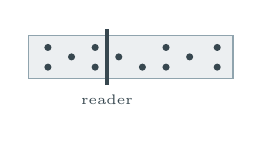
\begin{tikzpicture}
  \draw[draw=nLine, fill=nFill] (0,0) rectangle (2.6,0.55);
  \foreach \x/\y in {0.25/0.15,0.25/0.4,0.55/0.28,0.85/0.15,0.85/0.4,1.15/0.28,1.45/0.15,1.75/0.4,1.75/0.15,2.05/0.28,2.4/0.15,2.4/0.4}
    {\fill[nInk] (\x,\y) circle (0.045);}
  \draw[nInk, very thick] (1.0,-0.08) -- (1.0,0.63);
  \node[font=\tiny, text=nInk, anchor=north] at (1.0,-0.08) {reader};
\end{tikzpicture}}

\newcommand{\diagMemStackSmall}{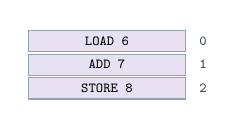
\begin{tikzpicture}
  \node[smallcell, fill=sViolet!18, minimum width=2.0cm] at (0,0.3) {LOAD 6};
  \node[smallcell, fill=sViolet!18, minimum width=2.0cm] at (0,0) {ADD 7};
  \node[smallcell, fill=sViolet!18, minimum width=2.0cm] at (0,-0.3) {STORE 8};
  \node[addr, font=\ttfamily\tiny, anchor=west] at (1.05,0.3) {0};
  \node[addr, font=\ttfamily\tiny, anchor=west] at (1.05,0) {1};
  \node[addr, font=\ttfamily\tiny, anchor=west] at (1.05,-0.3) {2};
\end{tikzpicture}}

\newcommand{\diagTwoMem}{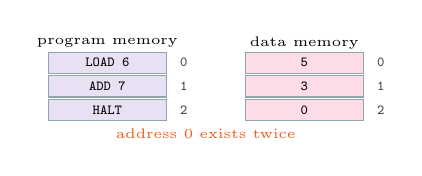
\begin{tikzpicture}
  \node[font=\tiny] at (0,0.55) {program memory};
  \node[font=\tiny] at (2.5,0.55) {data memory};
  \node[smallcell, fill=sViolet!18, minimum width=1.5cm] at (0,0.3) {LOAD 6};
  \node[smallcell, fill=sViolet!18, minimum width=1.5cm] at (0,0) {ADD 7};
  \node[smallcell, fill=sViolet!18, minimum width=1.5cm] at (0,-0.3) {HALT};
  \node[smallcell, fill=sPink!18, minimum width=1.5cm] at (2.5,0.3) {5};
  \node[smallcell, fill=sPink!18, minimum width=1.5cm] at (2.5,0) {3};
  \node[smallcell, fill=sPink!18, minimum width=1.5cm] at (2.5,-0.3) {0};
  \foreach \i in {0,1,2} {
    \node[addr, font=\ttfamily\tiny, anchor=west] at (0.8,{0.3-0.3*\i}) {\i};
    \node[addr, font=\ttfamily\tiny, anchor=west] at (3.3,{0.3-0.3*\i}) {\i};
  }
  \node[font=\tiny, text=AccentOrange] at (1.25,-0.6) {address 0 exists twice};
\end{tikzpicture}}

\newcommand{\diagOneMem}{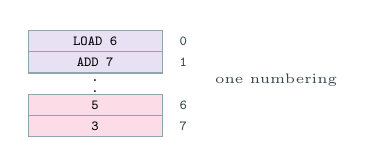
\begin{tikzpicture}
  \node[smallcell, fill=sViolet!18, minimum width=1.7cm] (o0) at (0,0.5) {LOAD 6};
  \node[smallcell, fill=sViolet!18, minimum width=1.7cm] at (0,0.23) {ADD 7};
  \node[smallcell, draw=none, minimum width=1.7cm] at (0,-0.04) {$\vdots$};
  \node[smallcell, fill=sPink!18, minimum width=1.7cm] at (0,-0.31) {5};
  \node[smallcell, fill=sPink!18, minimum width=1.7cm] at (0,-0.58) {3};
  \node[addr, font=\ttfamily\tiny, anchor=west] at (0.95,0.5) {0};
  \node[addr, font=\ttfamily\tiny, anchor=west] at (0.95,0.23) {1};
  \node[addr, font=\ttfamily\tiny, anchor=west] at (0.95,-0.31) {6};
  \node[addr, font=\ttfamily\tiny, anchor=west] at (0.95,-0.58) {7};
  \node[font=\tiny, text=nInk, anchor=west] at (1.4,0) {one numbering};
\end{tikzpicture}}

\newcommand{\diagDecimal}{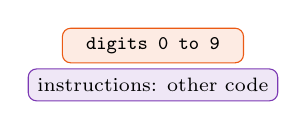
\begin{tikzpicture}
  \node[draw=AccentOrange, fill=AccentOrange!12, rounded corners=3pt, font=\ttfamily\scriptsize, minimum height=0.4cm,
    minimum width=2.3cm] at (0,0.28) {digits 0 to 9};
  \node[draw=ProgramPurple, fill=ProgramPurple!12, rounded corners=3pt, font=\scriptsize, minimum height=0.4cm,
    minimum width=2.3cm] at (0,-0.22) {instructions: other code};
\end{tikzpicture}}

\newcommand{\diagBinary}{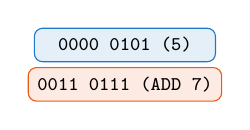
\begin{tikzpicture}
  \node[draw=StorageBlue, fill=StorageBlue!12, rounded corners=3pt, font=\ttfamily\scriptsize, minimum height=0.4cm,
    minimum width=2.3cm] at (0,0.28) {0000 0101 (5)};
  \node[draw=AccentOrange, fill=AccentOrange!12, rounded corners=3pt, font=\ttfamily\scriptsize, minimum height=0.4cm,
    minimum width=2.3cm] at (0,-0.22) {0011 0111 (ADD 7)};
\end{tikzpicture}}

\newcommand{\diagParallel}{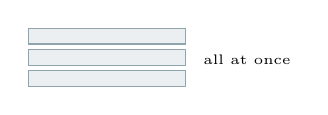
\begin{tikzpicture}
  \foreach \k in {0,1,2} {\draw[fill=nFill, draw=nLine] (0,{0.6-0.27*\k}) rectangle (2.0,{0.4-0.27*\k});}
  \node[font=\tiny, anchor=west] at (2.1,0.2) {all at once};
\end{tikzpicture}}

\newcommand{\diagDataflow}{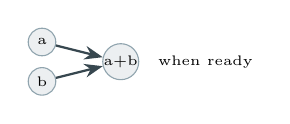
\begin{tikzpicture}[>=Stealth]
  \node[circle, draw=nLine, fill=nFill, minimum size=0.35cm, inner sep=0pt, font=\tiny] (a) at (0,0.3) {a};
  \node[circle, draw=nLine, fill=nFill, minimum size=0.35cm, inner sep=0pt, font=\tiny] (b) at (0,-0.2) {b};
  \node[circle, draw=nLine, fill=nFill, minimum size=0.4cm, inner sep=0pt, font=\tiny] (c) at (1.0,0.05) {a+b};
  \draw[->, thick, nInk] (a) -- (c); \draw[->, thick, nInk] (b) -- (c);
  \node[font=\tiny, anchor=west] at (1.35,0.05) {when ready};
\end{tikzpicture}}

\newcommand{\diagSequential}{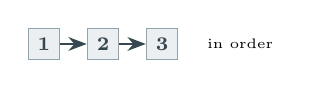
\begin{tikzpicture}[>=Stealth]
  \foreach \k in {1,2,3} {\node[draw=nLine, fill=nFill, text=nInk, minimum size=0.4cm, inner sep=0pt, font=\scriptsize\bfseries]
    (s\k) at ({0.75*\k-0.75},0.05) {\k};}
  \draw[->, thick, nInk] (s1) -- (s2); \draw[->, thick, nInk] (s2) -- (s3);
  \node[font=\tiny, anchor=west] at (1.95,0.05) {in order};
\end{tikzpicture}}

\newcommand{\diagMonolith}{
\begin{tikzpicture}
  \node[draw=nLine, very thick, rounded corners=4pt, fill=nFill, text=nInk, minimum width=2.6cm, minimum height=0.85cm,
    font=\scriptsize, align=center] {one block:\\[-1pt]everything mixed together};
\end{tikzpicture}}

\newcommand{\diagUnits}{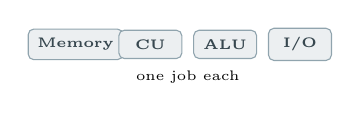
\begin{tikzpicture}
  \node[draw=nLine, fill=nFill, text=nInk, rounded corners=2pt, font=\tiny\bfseries, minimum width=0.8cm, minimum height=0.36cm] at (0,0.22) {Memory};
  \node[draw=nLine, fill=nFill, text=nInk, rounded corners=2pt, font=\tiny\bfseries, minimum width=0.8cm, minimum height=0.36cm] at (0.95,0.22) {CU};
  \node[draw=nLine, fill=nFill, text=nInk, rounded corners=2pt, font=\tiny\bfseries, minimum width=0.8cm, minimum height=0.36cm] at (1.9,0.22) {ALU};
  \node[draw=nLine, fill=nFill, text=nInk, rounded corners=2pt, font=\tiny\bfseries, minimum width=0.8cm, minimum height=0.36cm] at (2.85,0.22) {I/O};
  \node[font=\tiny] at (1.425,-0.2) {one job each};
\end{tikzpicture}}

% ---------- helpers for the CPU section ----------
\tikzset{
  reg/.style={draw=nLine, very thick, fill=white, text=nInk, rounded corners=2pt,
    minimum width=1.95cm, minimum height=0.55cm, inner sep=2pt, font=\ttfamily\scriptsize, align=center},
  cpuunit/.style={very thick, rounded corners=3pt, minimum width=1.2cm, minimum height=0.6cm,
    inner sep=2pt, font=\scriptsize\bfseries, align=center},
  hot/.style={aexec, label={[text=aExec, inner sep=1pt, font=\tiny]right:$\blacktriangleleft$}},
  hotdata/.style={aread},
  hotwrite/.style={awrite},
  hotalu/.style={aexec},
  fetcharrow/.style={-{Stealth}, very thick, DeepBlue, rounded corners=3pt},
  dataarrow/.style={-{Stealth}, very thick, DeepBlue, rounded corners=3pt},
  steplabel/.style={font=\tiny\bfseries, fill=white, inner sep=1pt},
}
% memory with the running example
% #1 highlighted instruction (0-3, -1 = none)  #2 text of cell 8  #3 highlighted data cell (6-8, 0 = none)
\newcommand{\mempanel}[3]{%
  \node[font=\scriptsize\bfseries, text=nInk] at (0,1.8) {Memory};
  \foreach \i/\t in {0/{0001 0110\ \ LOAD 6},1/{0011 0111\ \ ADD 7},2/{0010 1000\ \ STORE 8},3/{0111 0000\ \ HALT}} {
    \ifnum\i=#1
      \node[instrcell, minimum width=2.9cm, hot] (m\i) at (0,{1.35-0.45*\i}) {\t};
    \else
      \node[instrcell, minimum width=2.9cm] (m\i) at (0,{1.35-0.45*\i}) {\t};
    \fi
    \node[addr, anchor=east] at (-1.5,{1.35-0.45*\i}) {\i};
  }
  \node[memcell, draw=none, minimum width=2.9cm] at (0,-0.45) {$\vdots$};
  \foreach \i/\t/\y in {6/{0000 0101\ \ (5)}/-0.9,7/{0000 0011\ \ (3)}/-1.35,8/{#2}/-1.8} {
    \ifnum\i=#3
      \ifnum\i=8 \node[datacell, minimum width=2.9cm, hotwrite] (m\i) at (0,\y) {\t};\else \node[datacell, minimum width=2.9cm, hotdata] (m\i) at (0,\y) {\t};\fi
    \else
      \node[datacell, minimum width=2.9cm] (m\i) at (0,\y) {\t};
    \fi
    \node[addr, anchor=east] at (-1.5,\y) {\i};
  }
}
% the CPU, built up step by step
% #1 level: 0 empty, 1 +PC, 2 +IR, 3 +AC, 4 +ALU, 5 +CU   #2 PC   #3 IR   #4 AC   #5 extra ALU style
\newcommand{\cpupanel}[5]{%
  \node[draw=nLine, very thick, rounded corners=6pt, fill=nFill!50, minimum width=4.65cm,
    minimum height=3.85cm, anchor=west] (cpu) at (2.45,-0.2) {};
  \node[font=\scriptsize\bfseries, text=nInk, anchor=north west] at ([shift={(0.1,-0.06)}]cpu.north west) {CPU};
  \ifnum#1>0 \node[reg] (pc) at (3.65,0.95) {\textbf{PC}\ \ #2}; \fi
  \ifnum#1>1 \node[reg] (ir) at (3.65,0.0) {\textbf{IR}\\[-1pt]#3}; \fi
  \ifnum#1>2 \node[reg] (ac) at (3.65,-1.05) {\textbf{AC}\ \ #4}; \fi
  \ifnum#1>3 \node[cpuunit, draw=mygreen, fill=mygreen!18, #5] (alu) at (6.3,-1.05)
    {\textcolor{mygreen!60!black}{\faCalculator}\\[-1pt]ALU}; \fi
  \ifnum#1>4 \node[cpuunit, draw=AccentOrange, fill=AccentOrange!18] (cu) at (6.3,0.5)
    {\textcolor{AccentOrange}{\faCogs}\\[-1pt]CU}; \fi
}
% explanation slide: #1 title, #2 tikz body (memory + CPU), #3 right-hand column
\newcommand{\explainframe}[3]{%
\begin{frame}{#1}
  \begin{columns}[c,onlytextwidth]
    \column{0.58\textwidth}
      \centering
      \begin{tikzpicture}[>=Stealth, scale=0.92, every node/.append style={transform shape}]
        #2
      \end{tikzpicture}
    \column{0.4\textwidth}
      #3
  \end{columns}
\end{frame}}
% boxes for the right-hand column
\newcommand{\defbox}[1]{%
  \begin{beamercolorbox}[rounded=true,sep=0.1cm,wd=\linewidth]{block body example}
    \footnotesize #1
  \end{beamercolorbox}\vspace{0.06cm}}
\newcommand{\stepbox}[2]{%
  \begin{beamercolorbox}[rounded=true,sep=0.09cm,wd=\linewidth]{block body}
    \footnotesize\textbf{#1}\\ #2
  \end{beamercolorbox}\vspace{0.06cm}}
\newcommand{\phasename}[1]{%
  {\centering\footnotesize Name of this phase:\ \colorbox{DeepBlue}{\textcolor{white}{\textbf{#1}}}\par}}
% small tag above the CPU box: which instruction is being executed
\newcommand{\executing}[1]{%
  \node[font=\scriptsize\bfseries, text=AccentOrange, anchor=south east] at ([yshift=1pt]cpu.north east)
    {Executing: \texttt{#1}};}
\newcommand{\statebox}[1]{%
  {\centering\scriptsize\textcolor{DeepBlue}{\textbf{State:}}\ #1\par}}

\lstset{
  language=Python,
  basicstyle=\color{VSText}\ttfamily\footnotesize,
  keywordstyle=\color{VSPurple}\bfseries,
  stringstyle=\color{VSString},
  commentstyle=\color{VSComment}\itshape,
  numbers=left,
  numberstyle=\tiny\color{gray},
  stepnumber=1,
  breaklines=true,
  showstringspaces=false,
  xleftmargin=15pt,
  xrightmargin=5pt,
  frame=none
}

% MARIE assembly: line numbers start at 0, so a line number equals the memory address
\lstdefinelanguage{MARIE}{
  morekeywords={Load,Store,Add,Subt,Input,Output,Halt,Jump,Skipcond,DEC,HEX,ADR,LoadI,StoreI,AddI,JumpI,JnS,Clear,LoadImmi},
  sensitive=false,
  comment=[l]{/},
}
\lstdefinestyle{marie}{language=MARIE, firstnumber=0, basicstyle=\color{VSText}\ttfamily\scriptsize,
  keywordstyle=\color{VSBlue}\bfseries, commentstyle=\color{VSComment}\itshape,
  columns=fixed, basewidth=0.52em, keepspaces=true, breaklines=false, xleftmargin=12pt}

\BeforeBeginEnvironment{lstlisting}{%
  \begin{beamercolorbox}[rounded=true,sep=2mm,wd=\linewidth]{vscodelisting}%
  
\begin{tikzpicture}
    \fill[nLine] (0,0) circle (3pt);
    \fill[nLine] (0.35,0) circle (3pt);
    \fill[nLine] (0.70,0) circle (3pt);
  \end{tikzpicture}%
  \vspace{-0.2cm}%
}
\AfterEndEnvironment{lstlisting}{\end{beamercolorbox}}

% =====================================================================
%  Day 2 helpers
% =====================================================================

% ---------- MARIE datapath, drawn like the Data Path view of MARIE.js ----------
% \busdiagram[values]{source}{destination}{extra TikZ}
%   source (Read, blue) and destination (Write, red): ir, out, in, ac, mbr, pc, mar, mem, none
%   values: ir=, out=, in=, ac=, mbr=, pc=, mar=, mem= (contents of M[MAR]), step= (0-7, -1 = none)
\definecolor{ReadBlue}{HTML}{1E88E5}
\definecolor{WriteRed}{HTML}{E53935}
\definecolor{BusGreen}{HTML}{B0BEC5}% the bus: neutral
\tikzset{
  dpreg/.style={draw=nLine, thick, fill=white, text=nInk, minimum width=1.1cm, minimum height=0.46cm,
    inner sep=1pt, font=\ttfamily\scriptsize},
  dpname/.style={font=\tiny, text=nInk, above=0pt, inner sep=1pt},
  dpwire/.style={thin, nLight},
  dpmem/.style={draw=nLine, very thick, fill=nFill, rounded corners=3pt,
    minimum width=1.3cm, minimum height=0.95cm, font=\scriptsize\bfseries, align=center},
  srcreg/.style={draw=ReadBlue, line width=1.6pt},
  dstreg/.style={draw=WriteRed, line width=1.6pt},
}
\pgfkeys{/dp/.is family, /dp,
  ir/.initial={0000}, out/.initial={0000}, in/.initial={0000}, ac/.initial={0000},
  mbr/.initial={0000}, pc/.initial={000}, mar/.initial={000}, mem/.initial={0000},
  step/.initial={-1}}
\newcommand{\dpv}[1]{\pgfkeysvalueof{/dp/#1}}
\newcommand{\busdiagram}[4][]{%
  \begingroup
  \pgfkeys{/dp, ir=0000, out=0000, in=0000, ac=0000, mbr=0000, pc=000, mar=000, mem=0000, step=-1, #1}%
  \begin{tikzpicture}[>=Stealth]
    \tikzset{bd-mem/.style={}, bd-mar/.style={}, bd-pc/.style={}, bd-mbr/.style={},
      bd-ac/.style={}, bd-ir/.style={}, bd-in/.style={}, bd-out/.style={}, bd-none/.style={}}
    \tikzset{bd-#2/.style={srcreg}}
    \tikzset{bd-#3/.style={dstreg}}
    % ----- control unit -----
    \node[draw=DeepBlue!80, thick, fill=white, minimum width=1.3cm, minimum height=2.95cm,
      anchor=north west] (cu) at (-2.4,2.0) {};
    \node[font=\tiny, text=DeepBlue, anchor=north west, below=1pt] at (cu.south west) {Control unit};
    \node[font=\tiny, text=DeepBlue!80, anchor=east] at (-1.15,1.75) {Read};
    \node[font=\tiny, text=DeepBlue!80, anchor=east] at (-1.15,-0.6) {Write};
    \node[font=\tiny, text=DeepBlue!80, anchor=east] at (-1.15,0.05) {AC<0};
    \node[font=\tiny, text=DeepBlue!80, anchor=east] at (-1.15,-0.15) {AC=0};
    \node[font=\tiny, text=DeepBlue!80] at (-2.0,1.3) {Step};
    \foreach \k in {0,...,7} {
      \pgfmathtruncatemacro{\cur}{\dpv{step}}
      \ifnum\k=\cur
        \fill[AccentOrange] (-2.0,{1.1-0.15*\k}) circle (0.065);
      \else
        \fill[DeepBlue!30] (-2.0,{1.1-0.15*\k}) circle (0.035);
      \fi
    }
    % ----- memory -----
    \node[draw=DeepBlue!80, thick, fill=white, minimum width=1.5cm, minimum height=2.95cm,
      anchor=north west, bd-mem] (mem) at (10.4,2.0) {};
    \node[font=\tiny, text=DeepBlue, anchor=north west, below=1pt] at (mem.south west) {Main memory};
    \node[font=\ttfamily\tiny, text=DeepBlue!80] at (11.15,0.75) {M[MAR]};
    \node[font=\ttfamily\scriptsize] at (11.15,0.5) {\dpv{mem}};
    % ----- faint control wires (one Read and one Write wire per device) -----
    \draw[dpwire] (-1.1,1.75) -- (10.4,1.75);
    \draw[dpwire] (-1.1,-0.6) -- (10.4,-0.6);
    \foreach \x in {0.6,2.0,3.4,4.8,6.2,7.6,9.0} {
      \draw[dpwire] (\x-0.25,1.75) -- (\x-0.25,1.18);
      \draw[dpwire] (\x+0.3,-0.6) -- (\x+0.3,0.72);
    }
    % ----- bus (drawn first, registers on top) -----
    \foreach \x in {0.6,2.0,3.4,4.8,6.2,7.6,9.0}
      \draw[line width=2.6pt, BusGreen] (\x,0.72) -- (\x,-0.35);
    \draw[line width=2.6pt, BusGreen] (0.6-0.045,-0.35) -- (10.4,-0.35);
    % ----- ALU between AC and MBR, with its links and the flag wires to the CU -----
    \draw[thin, DeepBlue!40] (4.45,0.05) -- (-1.1,0.05);
    \draw[thin, DeepBlue!40] (4.45,-0.15) -- (-1.1,-0.15);
    \draw[thick, DeepBlue!70, fill=white] (5.0,0.47) -- (5.42,0.47) -- (5.5,0.37) -- (5.58,0.47) -- (6.0,0.47)
      -- (5.72,0.05) -- (5.28,0.05) -- cycle;
    \node[font=\tiny, text=DeepBlue!80] at (5.5,0.22) {ALU};
    \draw[thick, DeepBlue!60] (5.2,0.72) -- (5.2,0.47);
    \draw[thick, DeepBlue!60] (5.8,0.72) -- (5.8,0.47);
    \draw[thick, DeepBlue!60] (5.5,0.05) -- (5.5,-0.1) -- (4.45,-0.1) |- (4.45,0.72);
    % ----- registers -----
    \foreach \n/\x/\lab in {ir/0.6/IR, out/2.0/OUT, in/3.4/IN, ac/4.8/AC, mbr/6.2/MBR, pc/7.6/PC, mar/9.0/MAR} {
      \node[dpreg, bd-\n] (\n) at (\x,0.95) {\dpv{\n}};
      \node[dpname] at (\n.north) {\lab};
      \coordinate (\n-port) at (\n.south);
      \coordinate (\n-bus) at (\x,-0.35);
    }
    \coordinate (mem-port) at (10.4,-0.35);
    \coordinate (mem-bus) at (10.4,-0.35);
    % IR is decoded by the CU; MAR selects the memory cell
    \draw[thick, BusGreen, -{Stealth}] (ir.west) -- (-1.1,0.95);
    \draw[thick, BusGreen, -{Stealth}] (mar.east) -- (10.4,0.95);
    % ----- active Read and Write signals -----
    \ifstrequal{#2}{none}{}{%
      \ifstrequal{#2}{mem}
        {\draw[line width=1.3pt, ReadBlue, -{Stealth}] (-1.1,1.75) -- (10.4,1.75);}
        {\draw[line width=1.3pt, ReadBlue, -{Stealth}] (-1.1,1.75) -| ($(#2.north)+(-0.25,0)$);}}
    \ifstrequal{#3}{none}{}{%
      \ifstrequal{#3}{mem}
        {\draw[line width=1.3pt, WriteRed, -{Stealth}] (-1.1,-0.6) -- (10.4,-0.6);}
        {\draw[line width=1.3pt, WriteRed, -{Stealth}] (-1.1,-0.6) -| ($(#3.south)+(0.3,0)$);}}
    % ----- the value travelling along the bus -----
    \ifstrequal{#2}{none}{}{\ifstrequal{#3}{none}{}{%
      \draw[line width=3pt, nInk] (#2-port) -- (#2-bus) -- (#3-bus) -- (#3-port);
      \draw[line width=1.5pt, white, dash pattern=on 1.5pt off 1.5pt] (#2-port) -- (#2-bus) -- (#3-bus) -- (#3-port);}}
    #4
  \end{tikzpicture}%
  \endgroup}

% legend for the colours of the data path
\newcommand{\dplegend}{%
  {\tiny\textcolor{ReadBlue}{\rule{0.25cm}{0.2cm}}\ \textbf{Read}: puts its value on the bus
  \qquad\textcolor{WriteRed}{\rule{0.25cm}{0.2cm}}\ \textbf{Write}: stores the value from the bus
  \qquad\tikz[baseline=-0.6ex]{\draw[line width=3pt, BusGreen] (0,0) -- (0.5,0);\draw[line width=1.5pt, white, dash pattern=on 1.5pt off 1.5pt] (0,0) -- (0.5,0);}\ the value travelling on the bus}}

% one step of an instruction: data path on top, explanation below
% #1 title, #2 source, #3 destination, #4 values (keys), #5 explanation
\newcommand{\stepframe}[5]{%
\begin{frame}{#1}
  \begin{center}
    \resizebox{0.8\textwidth}{!}{\busdiagram[#4]{#2}{#3}{}}\\[0.02cm]
    \dplegend
  \end{center}
  \vspace{-0.1cm}
  \begin{center}
    \begin{minipage}{0.8\textwidth}
      #5
    \end{minipage}
  \end{center}
\end{frame}}

% ---------- timeline of clock steps ----------
% #1 fetch steps, #2 execute steps, #3 label on the right
\newcommand{\steptimeline}[3]{%
  \begin{tikzpicture}
    \foreach \i in {1,...,#1}
      \node[draw=white, fill=sAmber, text=black, font=\tiny\bfseries, minimum width=0.62cm,
        minimum height=0.45cm, inner sep=0pt] at ({0.62*(\i-1)},0) {T\the\numexpr\i-1\relax};
    \foreach \i in {1,...,#2}
      \node[draw=white, fill=sTeal, text=white, font=\tiny\bfseries, minimum width=0.62cm,
        minimum height=0.45cm, inner sep=0pt] at ({0.62*(#1+\i-1)},0) {T\the\numexpr#1+\i-1\relax};
    \node[anchor=west, font=\scriptsize] at ({0.62*(#1+#2)-0.25},0) {#3};
  \end{tikzpicture}}

% legend for the timeline colours
\newcommand{\timelinelegend}{%
  {\tiny\textcolor{StorageBlue!75}{\rule{0.25cm}{0.2cm}}\ fetch
  \qquad\textcolor{AccentOrange}{\rule{0.25cm}{0.2cm}}\ execute}}

% ---------- small pieces for the addressing-mode slides ----------
\tikzset{
  mcell/.style={draw=DeepBlue!60, minimum width=1.5cm, minimum height=0.42cm, inner sep=1pt,
    font=\ttfamily\scriptsize, align=center, fill=StorageBlue!15},
  mcellhot/.style={mcell, fill=StorageBlue!45, draw=StorageBlue, very thick},
  mcellptr/.style={mcell, fill=ProgramPurple!18, draw=ProgramPurple, very thick},
  instrbox/.style={draw=AccentOrange, very thick, fill=AccentOrange!15, rounded corners=2pt,
    minimum height=0.5cm, inner sep=3pt, font=\ttfamily\scriptsize},
  ptrarrow/.style={-{Stealth}, very thick, DeepBlue},
  valarrow/.style={-{Stealth}, very thick, DeepBlue},
}

% task header box (same look as on Day 1)
% #1 form and time, #2 short instruction
\newcommand{\taskhead}[2]{%
  \begin{beamercolorbox}[rounded=true,sep=0.12cm,wd=\linewidth]{block body example}
    \small\textbf{#1}\\[0.04cm]
    \footnotesize #2
  \end{beamercolorbox}\vspace{0.1cm}}

% highlighted key message at the bottom of a slide
\newcommand{\keymsg}[1]{%
  \begin{beamercolorbox}[rounded=true,sep=0.1cm,wd=\textwidth]{block body example}
    \centering\footnotesize #1
  \end{beamercolorbox}}

% register transfer written in text: \mo{MAR}{PC} gives MAR <- PC
\newcommand{\mo}[2]{\texttt{#1\,$\leftarrow$\,#2}}

% plain listings (x86, RISC-V) without Python highlighting
\lstdefinelanguage{plain}{}
\lstdefinestyle{asm}{language=plain, basicstyle=\color{VSText}\ttfamily\scriptsize, numbers=none,
  columns=fixed, basewidth=0.52em, keepspaces=true, xleftmargin=6pt}

% =====================================================================
%  Day 3 helpers
% =====================================================================

\usetikzlibrary{patterns}
\usepackage{multirow}
% ---------- RISC-V listings ----------
\lstdefinestyle{rv}{language=RISCV, basicstyle=\color{VSText}\ttfamily\scriptsize, numbers=none,
  keywordstyle=\color{VSBlue}\bfseries, keywordstyle={[2]\color{VSPurple}\bfseries},
  commentstyle=\color{VSComment}\itshape,
  columns=fixed, basewidth=0.52em, keepspaces=true, breaklines=false, xleftmargin=6pt}
\lstdefinestyle{rvnum}{style=rv, numbers=left, firstnumber=1, xleftmargin=14pt}

% ---------- colours of the five pipeline stages (the same all day) ----------
\colorlet{cIF}{sAmber}
\colorlet{cID}{sBrown}
\colorlet{cEX}{sTeal}
\colorlet{cMEM}{sIndigo}
\colorlet{cWB}{sPink}
% text on a stage colour (amber needs black)
\colorlet{txIF}{black}\colorlet{txID}{white}\colorlet{txEX}{white}\colorlet{txMEM}{white}\colorlet{txWB}{white}
\colorlet{txcIF}{black}\colorlet{txcID}{white}\colorlet{txcEX}{white}\colorlet{txcMEM}{white}\colorlet{txcWB}{white}

% ---------- pipeline diagrams ----------
% cell size (cm)
\def\pw{0.74}
\def\ph{0.46}
\tikzset{
  pcell/.style={minimum width=\pw cm, minimum height=\ph cm, inner sep=0pt, draw=white,
    font=\scriptsize\bfseries, text=white},
  pst-IF/.style={pcell, fill=cIF, text=black},
  pst-ID/.style={pcell, fill=cID},
  pst-EX/.style={pcell, fill=cEX},
  pst-MEM/.style={pcell, fill=cMEM},
  pst-WB/.style={pcell, fill=cWB},
  pst-B/.style={pcell, fill=nIdle, text=nInk, font=\tiny},
  pst-X/.style={pcell, fill=nFill, text=nInk, draw=nLine},
  pst-N/.style={pcell, fill=none, draw=none},
  pst-E/.style={pcell, fill=nFill!60},
  plab/.style={anchor=east, font=\ttfamily\footnotesize, inner sep=1pt},
}
% one row of a pipeline diagram
% #1 row (0 = top), #2 first cycle (1-based), #3 comma list of IF, ID, EX, MEM, WB, B (bubble), X (flushed), N (empty)
\newcommand{\prow}[3]{%
  \foreach \s [count=\k from 0] in {#3} {%
    \node[pst-\s] at ({(#2+\k-1)*\pw}, {-(#1)*\ph}) {%
      \expandafter\ifstrequal\expandafter{\s}{B}{bubble}{%
      \expandafter\ifstrequal\expandafter{\s}{X}{$\times$}{%
      \expandafter\ifstrequal\expandafter{\s}{N}{}{\expandafter\ifstrequal\expandafter{\s}{E}{}{\s}}}}};
  }}
% label of a row
\newcommand{\plabel}[2]{\node[plab] at ({-0.5*\pw-0.05}, {-(#1)*\ph}) {#2};}
% cycle numbers above the diagram: #1 number of cycles
\newcommand{\pcycles}[1]{%
  \foreach \c in {1,...,#1}
    \node[font=\scriptsize, text=DeepBlue!70] at ({(\c-1)*\pw}, {0.8*\ph}) {\c};
  \node[font=\scriptsize, text=DeepBlue!70, anchor=east] at ({-0.5*\pw-0.05}, {0.8*\ph}) {cycle};}
% highlight one column: #1 cycle, #2 number of rows, #3 colour
\newcommand{\pcolumn}[3]{%
  \draw[#3, very thick, rounded corners=2pt]
    ({(#1-1.5)*\pw}, {0.5*\ph}) rectangle ({(#1-0.5)*\pw}, {-(#2-0.5)*\ph});}

% legend of stage colours
\newcommand{\stagelegend}{%
  {\tiny
  \textcolor{cIF}{\rule{0.25cm}{0.2cm}}\,IF fetch\quad
  \textcolor{cID}{\rule{0.25cm}{0.2cm}}\,ID decode\quad
  \textcolor{cEX}{\rule{0.25cm}{0.2cm}}\,EX execute\quad
  \textcolor{cMEM}{\rule{0.25cm}{0.2cm}}\,MEM memory\quad
  \textcolor{cWB}{\rule{0.25cm}{0.2cm}}\,WB write back}}

% ---------- stage boxes ----------
\tikzset{
  stagebox/.style={very thick, rounded corners=4pt, minimum width=1.9cm, minimum height=0.8cm,
    align=center, font=\small\bfseries, drop shadow},
  gbar/.style={minimum height=0.36cm, inner sep=0pt, draw=white, font=\tiny\bfseries, text=white},
  gempty/.style={minimum height=0.36cm, inner sep=0pt, draw=gray!50, dashed, font=\tiny, text=gray!60},
  unit/.style={draw=nLine, very thick, fill=white, text=nInk, rounded corners=3pt, align=center,
    font=\scriptsize\bfseries, inner sep=2pt},
}

% ---------- a simple RISC-V datapath ----------
% #1 extra TikZ drawn on top (nodes: pc, imem, rf, alu, dmem, mux, cu, add4)
\newcommand{\rvdatapath}[1]{%
  \begin{tikzpicture}[>=Stealth, font=\scriptsize]
    % stage labels
    \foreach \x/\n/\c in {0.9/IF/cIF, 4.2/ID/cID, 6.6/EX/cEX, 9.0/MEM/cMEM, 10.9/WB/cWB}
      \node[fill=\c, text=tx\c, rounded corners=2pt, font=\tiny\bfseries, minimum width=0.9cm] at (\x,2.35) {\n};
    % units
    \node[unit, minimum width=0.6cm, minimum height=1.0cm] (pc) at (0,0) {PC};
    \node[unit, minimum width=1.5cm, minimum height=1.6cm] (imem) at (1.8,0) {Instruction\\memory};
    \node[unit, minimum width=1.5cm, minimum height=1.8cm] (rf) at (4.2,0) {Register\\file};
    \draw[nInk, very thick, fill=white] (6.2,0.9) -- (7.0,0.45) -- (7.0,-0.45) -- (6.2,-0.9) -- (6.2,-0.25)
      -- (6.4,0) -- (6.2,0.25) -- cycle;
    \node[font=\scriptsize\bfseries] (alu) at (6.68,0) {ALU};
    \coordinate (aluin1) at (6.2,0.55); \coordinate (aluin2) at (6.2,-0.55); \coordinate (aluout) at (7.0,0);
    \node[unit, minimum width=1.5cm, minimum height=1.6cm] (dmem) at (9.0,0) {Data\\memory};
    \node[unit, minimum width=0.45cm, minimum height=1.2cm, rounded corners=6pt, font=\tiny] (mux) at (10.9,0) {M\\U\\X};
    \node[unit, minimum width=1.3cm, minimum height=0.5cm, draw=nLine, text=nLine] (add4) at (0.9,1.55) {$+4$};
    \node[unit, minimum width=2.2cm, minimum height=0.5cm, draw=gray, text=gray] (cu) at (4.2,-1.85) {Control unit};
    % wires
    \draw[->, thick] (pc) -- (imem);
    \draw[->, thick] (imem) -- node[above, font=\tiny] {instruction} (rf);
    \draw[->, thick] ([yshift=0.55cm]rf.east) -- (aluin1);
    \draw[->, thick] ([yshift=-0.55cm]rf.east) -- (aluin2);
    \draw[->, thick] (aluout) -- node[above, font=\tiny] {address} ([yshift=0cm]dmem.west);
    \draw[->, thick] ([yshift=-0.55cm]dmem.east) -- ([yshift=-0.4cm]mux.west);
    \draw[->, thick] (7.3,0) |- (7.3,-1.1) -| (10.3,-1.1) |- ([yshift=0.4cm]mux.west);
    \draw[->, thick] (mux.east) -- ++(0.3,0) |- (11.2,2.0) -| node[pos=0.25, above, font=\tiny] {write back} (4.2,0.9);
    \draw[->, thick, DeepBlue!60] (pc.north) |- (add4.west);
    \draw[->, thick, DeepBlue!60] (add4.east) -- ++(0.35,0) |- (-0.6,1.95) |- (pc.west);
    \draw[->, dashed, gray] (cu.north) -- (rf.south);
    \draw[->, dashed, gray] (cu.east) -| (dmem.south);
    \draw[->, dashed, gray] (cu.east) -| (mux.south);
    #1
  \end{tikzpicture}}

% ---------- Ripes window (schematic; replace with a real screenshot if you like) ----------
\newcommand{\ripeswindow}{%
  \begin{tikzpicture}[font=\tiny]
    \draw[nInk, very thick, fill=white, rounded corners=4pt] (0,0) rectangle (9,5.4);
    \fill[nLight, rounded corners=4pt] (0,5.0) rectangle (9,5.4);
    \fill[MacRed] (0.25,5.2) circle (2.5pt); \fill[MacYellow] (0.5,5.2) circle (2.5pt); \fill[MacGreen] (0.75,5.2) circle (2.5pt);
    \node[font=\tiny\bfseries, text=nInk] at (4.5,5.2) {Ripes};
    % toolbar
    \fill[LightGray] (0,4.55) rectangle (9,5.0);
    \foreach \x/\i in {1.0/\faMicrochip, 1.6/\faStepForward, 2.2/\faPlay, 2.8/\faFastForward, 3.4/\faUndo}
      \node[text=nInk] at (\x,4.77) {\i};
    % side bar
    \fill[nLine] (0,0) rectangle (0.5,4.55);
    \foreach \y/\i in {4.1/\faEdit, 3.5/\faMicrochip, 2.9/\faMemory, 2.3/\faTerminal}
      \node[text=white] at (0.25,\y) {\i};
    % editor
    \draw[gray!60, fill=VSDarkBg] (0.65,0.15) rectangle (3.2,4.4);
    \foreach \y/\t in {4.1/lw x5{,} X, 3.8/lw x6{,} Y, 3.5/add x7{,} x5{,} x6, 3.2/addi x7{,} x7{,} -2, 2.9/sw x7{,} Z{,} x28}
      \node[anchor=west, text=VSText, font=\ttfamily\tiny] at (0.75,\y) {\t};
    % processor view
    \draw[gray!60, fill=nFill] (3.35,1.4) rectangle (7.3,4.4);
    \foreach \x/\c in {3.8/cIF, 4.5/cID, 5.3/cEX, 6.1/cMEM, 6.8/cWB}
      \draw[\c, very thick, fill=\c!15] (\x-0.25,2.3) rectangle (\x+0.25,3.6);
    \draw[->, thick, DeepBlue!60] (3.55,2.95) -- (7.05,2.95);
    \node[font=\tiny, text=nInk] at (5.3,1.85) {datapath};
    % statistics
    \draw[gray!60, fill=white] (3.35,0.15) rectangle (7.3,1.25);
    \node[anchor=west, font=\tiny] at (3.45,0.95) {Cycles: 13};
    \node[anchor=west, font=\tiny] at (3.45,0.7) {Instrs. retired: 8};
    \node[anchor=west, font=\tiny] at (3.45,0.45) {CPI: 1.63 \quad IPC: 0.62};
    % registers
    \draw[gray!60, fill=white] (7.45,0.15) rectangle (8.85,4.4);
    \foreach \k [count=\j from 0] in {x5,x6,x7,x8,x9,x10}
      \node[anchor=west, font=\ttfamily\tiny] at (7.5,{4.1-0.3*\j}) {\k};
    \node[font=\tiny, text=nInk] at (8.15,2.1) {registers};
    % badges
    \node[circle, fill=AccentOrange, text=white, font=\bfseries\scriptsize, inner sep=1.5pt] at (1.9,1.2) {1};
    \node[circle, fill=AccentOrange, text=white, font=\bfseries\scriptsize, inner sep=1.5pt] at (1.35,4.77) {2};
    \node[circle, fill=AccentOrange, text=white, font=\bfseries\scriptsize, inner sep=1.5pt] at (5.3,4.1) {3};
    \node[circle, fill=AccentOrange, text=white, font=\bfseries\scriptsize, inner sep=1.5pt] at (6.95,0.7) {4};
    \node[circle, fill=AccentOrange, text=white, font=\bfseries\scriptsize, inner sep=1.5pt] at (8.15,1.4) {5};
  \end{tikzpicture}}

% small orange number used in running text
\newcommand{\badge}[1]{\tikz[baseline=(b.base)]\node[circle,fill=AccentOrange,text=white,
  inner sep=1.2pt,font=\bfseries\tiny] (b) {#1};}

% =====================================================================
%  Day 4 helpers
% =====================================================================

% ---------- colours of the memory levels (the same all day) ----------
% memory levels are hardware: neutral
\colorlet{cReg}{nInk}
\colorlet{cCache}{nInk}
\colorlet{cRAM}{nLine}
\colorlet{cDisk}{nLine}
\colorlet{cIO}{nInk}
\colorlet{HitGreen}{aExec}
\colorlet{MissRed}{aWrite}
\setbeamercolor{block body answer}{bg=aExec!8,fg=black}

% ---------- listings ----------
% RISC-V: the Day 3 keywords plus the new ones used today
\lstdefinelanguage{RISCV}{
  morekeywords={lw,sw,add,addi,sub,beq,bne,bnez,beqz,la,li,auipc,nop,ecall},
  morekeywords=[2]{.data,.text,.word,.zero},
  alsoletter={.},
  sensitive=true,
  morecomment=[l]{\#},
}
% C (for the locality examples)
\lstdefinestyle{cc}{language=C, basicstyle=\color{VSText}\ttfamily\scriptsize, numbers=none,
  keywordstyle=\color{VSBlue}\bfseries, commentstyle=\color{VSComment}\itshape,
  columns=fixed, basewidth=0.52em, keepspaces=true, breaklines=false, xleftmargin=6pt,
  moredelim=**[is][\color{MacYellow}\bfseries]{@}{@}}

% ---------- boxes for the memory levels and devices ----------
\tikzset{
  lbox/.style={very thick, rounded corners=4pt, align=center, font=\scriptsize\bfseries, inner sep=3pt},
  cpubox/.style={lbox, draw=nInk, fill=nInk, text=white},
  regbox/.style={lbox, draw=nLine, fill=nFill, text=nInk},
  cachebox/.style={lbox, draw=nLine, fill=nFill, text=nInk},
  rambox/.style={lbox, draw=nLine, fill=nFill, text=nInk},
  diskbox/.style={lbox, draw=nLine, fill=nFill, text=nInk},
  iobox/.style={lbox, draw=cIO, fill=cIO!12},
  dmabox/.style={lbox, draw=nLine, fill=nFill, text=nInk},
  osbox/.style={lbox, draw=nLine, fill=nFill, text=nInk},
  greybox/.style={lbox, draw=nLight, fill=white, text=nLine},
  arr/.style={-{Stealth}, very thick, nInk},
  okarr/.style={-{Stealth}, very thick, HitGreen},
  badarr/.style={-{Stealth}, very thick, MissRed},
  smalltxt/.style={font=\tiny, inner sep=1pt},
}

% ---------- design question box (as on the Day 1 dilemma slides) ----------
\newcommand{\designq}[1]{%
  \begin{beamercolorbox}[rounded=true,sep=0.14cm,wd=\textwidth]{block body}
    \centering\small\textbf{Design question:} #1
  \end{beamercolorbox}}
\newcommand{\whichone}{%
  {\centering\small\textcolor{DeepBlue}{\textbf{Which would you choose, and why?}}\par}}

% ---------- question card and answer card ----------
% #1 icon, #2 text
\newcommand{\qcard}[2]{%
  \begin{beamercolorbox}[rounded=true,sep=0.14cm,wd=\linewidth]{block body}
    \centering{\Large\textcolor{AccentOrange}{#1}}\\[0.12cm]
    \footnotesize #2
  \end{beamercolorbox}}
% #1 title, #2 text
\newcommand{\acard}[2]{%
  \begin{beamercolorbox}[rounded=true,sep=0.1cm,wd=\linewidth]{block body answer}
    \footnotesize\textbf{\textcolor{aExec}{\faCheck}\ #1}\\ #2
  \end{beamercolorbox}\vspace{0.06cm}}
% red "problem" box
\setbeamercolor{block body problem}{bg=AccentOrange!10,fg=black}
\newcommand{\probbox}[2]{%
  \begin{beamercolorbox}[rounded=true,sep=0.09cm,wd=\linewidth]{block body problem}
    \footnotesize\textbf{\textcolor{AccentOrange}{\faExclamationTriangle}\ #1}\\ #2
  \end{beamercolorbox}\vspace{0.06cm}}

% ---------- hits and misses ----------
\def\cw{0.62}
\def\chh{0.42}
\tikzset{
  hmcell/.style={minimum width=\cw cm, minimum height=\chh cm, inner sep=0pt, draw=white,
    font=\scriptsize\bfseries, text=white},
  hm-H/.style={hmcell, fill=white, draw=nLight, text=aExec},
  hm-M/.style={hmcell, fill=white, draw=nLight, text=aWrite},
  hm-Q/.style={hmcell, fill=nFill, draw=nLight, text=nLine},
  hm-A/.style={hmcell, draw=none, text=nInk, font=\scriptsize\ttfamily\bfseries},
}
% one row of hits and misses: #1 row (0 = top), #2 comma list of H, M, Q (Q = to fill in)
\newcommand{\hmrow}[2]{%
  \foreach \s [count=\k from 0] in {#2} {%
    \node[hm-\s] at ({\k*\cw}, {-(#1)*\chh}) {\expandafter\ifstrequal\expandafter{\s}{Q}{?}{\s}};}}
% the accessed addresses above a row: #1 row, #2 comma list
\newcommand{\hmhead}[2]{%
  \foreach \s [count=\k from 0] in {#2}
    \node[hm-A] at ({\k*\cw}, {-(#1)*\chh}) {\s};}
% label on the left of a row: #1 row, #2 text
\newcommand{\hmlabel}[2]{\node[anchor=east, font=\scriptsize, inner sep=1pt] at ({-0.5*\cw-0.08}, {-(#1)*\chh}) {#2};}
% label on the right of a row: #1 row, #2 number of cells, #3 text
\newcommand{\hmresult}[3]{\node[anchor=west, font=\scriptsize\bfseries, text=nInk, inner sep=1pt]
  at ({(#2-0.5)*\cw+0.12}, {-(#1)*\chh}) {#3};}

% ---------- a small cache (or page table) drawn as a table ----------
\tikzset{
  ctab/.style={draw=nLine, text=nInk, minimum height=0.4cm, inner sep=1pt, font=\ttfamily\scriptsize, fill=white},
  ctabh/.style={ctab, fill=nInk, text=white, font=\scriptsize\bfseries},
  ctabhit/.style={fill=HitGreen!25, draw=HitGreen, very thick},
  ctabmiss/.style={fill=MissRed!20, draw=MissRed, very thick},
}
% #1 comma list of line/valid/tag/data ; columns: Line, V, Tag, Data (top-left corner at the origin)
\newcommand{\cachetable}[1]{%
  \node[ctabh, minimum width=0.9cm] at (0,0) {Line};
  \node[ctabh, minimum width=0.7cm] at (0.8,0) {V};
  \node[ctabh, minimum width=1.0cm] at (1.65,0) {Tag};
  \node[ctabh, minimum width=1.6cm] at (2.95,0) {Data};
  \foreach \xa/\xb/\xc/\xd [count=\k from 1] in {#1} {
    \node[ctab, minimum width=0.9cm] (cl\k) at (0,{-0.4*\k}) {\xa};
    \node[ctab, minimum width=0.7cm] (cv\k) at (0.8,{-0.4*\k}) {\xb};
    \node[ctab, minimum width=1.0cm] (ct\k) at (1.65,{-0.4*\k}) {\xc};
    \node[ctab, minimum width=1.6cm] (cd\k) at (2.95,{-0.4*\k}) {\xd};
  }}

% ---------- timelines (polling, interrupts, DMA, bus use) ----------
% #1 y, #2 label on the left, #3 comma list of length/colour/text
\newcommand{\tlbar}[3]{%
  \node[anchor=east, font=\scriptsize\bfseries, text=nInk, align=right] at (-0.1,#1) {#2};
  \gdef\tlx{0}%
  \foreach \tlw/\tlc/\tlt in {#3} {%
    \edef\tlcc{\tlc}\def\tlpoll{cPoll}\def\tlidle{cIdle}\def\tlb{cTaskB}%
    \def\tltext{white}\ifx\tlcc\tlpoll\def\tltext{nInk}\fi\ifx\tlcc\tlidle\def\tltext{nInk}\fi\ifx\tlcc\tlb\def\tltext{black}\fi
    \node[draw=white, fill=\tlc, minimum width=\tlw cm, minimum height=0.42cm, inner sep=0pt,
      anchor=west, font=\tiny\bfseries, text=\tltext] at (\tlx,#1) {\tlt};
    \pgfmathsetmacro{\tlnext}{\tlx+\tlw}%
    \xdef\tlx{\tlnext}%
  }}

% ---------- timing diagrams (buses) ----------
% a digital signal: #1 y, #2 label, #3 comma list of x/level pairs (level 0 or 1), #4 end x
\newcommand{\signal}[4]{%
  \node[anchor=east, font=\scriptsize\bfseries, text=nInk] at (-0.15,{#1+0.2}) {#2};
  \gdef\sgx{0}\gdef\sgl{0}%
  \foreach \sx/\sl in {#3} {%
    \draw[very thick, nInk] (\sgx,{#1+0.4*\sgl}) -- (\sx,{#1+0.4*\sgl}) -- (\sx,{#1+0.4*\sl});
    \xdef\sgx{\sx}\xdef\sgl{\sl}%
  }
  \draw[very thick, nInk] (\sgx,{#1+0.4*\sgl}) -- (#4,{#1+0.4*\sgl});}
% a bus value (address, data): #1 y, #2 label, #3 start x, #4 end x, #5 text, #6 colour
\newcommand{\busval}[6]{%
  \node[anchor=east, font=\scriptsize\bfseries, text=nInk, align=right] at (-0.15,{#1+0.2}) {#2};
  \fill[#6!20] (#3,#1+0.2) -- (#3+0.12,#1+0.4) -- (#4-0.12,#1+0.4) -- (#4,#1+0.2)
    -- (#4-0.12,#1) -- (#3+0.12,#1) -- cycle;
  \draw[very thick, #6] (#3,#1+0.2) -- (#3+0.12,#1+0.4) -- (#4-0.12,#1+0.4) -- (#4,#1+0.2)
    -- (#4-0.12,#1) -- (#3+0.12,#1) -- cycle;
  \node[font=\tiny\bfseries, text=#6!70!black] at ({(#3+#4)/2},{#1+0.2}) {#5};}
% a clock: #1 y, #2 number of periods, #3 period width
\newcommand{\clocksig}[3]{%
  \node[anchor=east, font=\scriptsize\bfseries, text=nInk] at (-0.15,{#1+0.2}) {Bus clock};
  \foreach \c in {1,...,#2} {
    \draw[very thick, nInk] ({(\c-1)*#3},#1) -- ({(\c-1)*#3},{#1+0.4}) -- ({(\c-0.5)*#3},{#1+0.4})
      -- ({(\c-0.5)*#3},#1) -- ({\c*#3},#1);
  }}
% a vertical time marker: #1 x, #2 top y, #3 bottom y, #4 label
\newcommand{\tmark}[4]{%
  \draw[nLine, dashed, thick] (#1,#2) -- (#1,#3);
  \node[font=\scriptsize\bfseries, text=AccentOrange, below] at (#1,#3) {#4};}

% ---------- latency bar on a log scale ----------
% #1 row, #2 label, #3 length (cm), #4 colour, #5 text at the end
\newcommand{\latbar}[5]{%
  \node[anchor=east, font=\scriptsize] at (-0.1,{-0.42*#1}) {#2};
  \fill[#4] (0,{-0.42*#1-0.15}) rectangle (#3,{-0.42*#1+0.15});
  \node[anchor=west, font=\scriptsize\bfseries, text=#4!80!black] at (#3+0.05,{-0.42*#1}) {#5};}

% =====================================================================
%  Day 5 helpers
% =====================================================================

% ---------- Arduino C++ listings (@...@ = part to change, shown in yellow) ----------
\lstdefinestyle{ino}{language=C++, basicstyle=\color{VSText}\ttfamily\scriptsize, numbers=none,
  keywordstyle=\color{VSBlue}\bfseries, commentstyle=\color{VSComment}\itshape, stringstyle=\color{VSString},
  columns=fixed, basewidth=0.52em, keepspaces=true, breaklines=false, showstringspaces=false, xleftmargin=6pt,
  morekeywords={uint8_t,uint32_t,IRAM_ATTR,HIGH,LOW,OUTPUT,INPUT_PULLUP,FALLING,hw_timer_t},
  emph={pinMode,digitalWrite,digitalRead,delay,millis,micros,attachInterrupt,digitalPinToInterrupt,
    timerBegin,timerAttachInterrupt,timerAlarm,memcpy,memcmp,memset,esp_async_memcpy,esp_async_memcpy_install},
  emphstyle=\color{VSPurple},
  moredelim=**[is][\color{MacYellow}\bfseries]{@}{@}}
% plain text in a dark box (serial monitor, terminal)
\lstdefinestyle{term}{language=plain, basicstyle=\color{VSText}\ttfamily\scriptsize, numbers=none,
  columns=fixed, basewidth=0.52em, keepspaces=true, xleftmargin=6pt,
  moredelim=**[is][\color{MacYellow}\bfseries]{@}{@}}

% ---------- colours used all day ----------
% who uses the CPU: main program indigo; checking the device = time lost (grey)
\colorlet{cWork}{sIndigo}
\colorlet{cPoll}{nIdle}
\colorlet{cISR}{sPink}
\colorlet{cCopy}{nLine}
\colorlet{cIdle}{nIdle}

% legend for the CPU timelines
\newcommand{\cpulegend}{%
  {\tiny\textcolor{cWork}{\rule{0.25cm}{0.2cm}}\ useful work
  \quad\textcolor{cPoll}{\rule{0.25cm}{0.2cm}}\ checking the device}}

% ---------- the ESP32-C3 board ----------
% the same Wokwi-style board as on the "Build it" slides (pic esp32c3, defined below)
\newcommand{\espboard}{%
  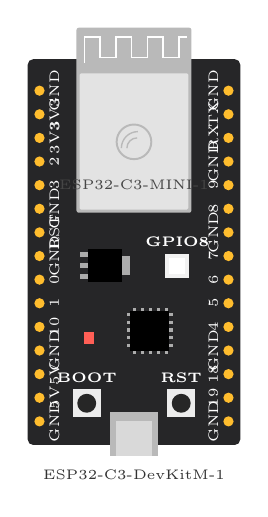
\begin{tikzpicture}
    \pic at (0,0) {esp32c3};
    \node[font=\tiny, text=gray!40!black, anchor=north] at (1.35,-0.2) {ESP32-C3-DevKitM-1};
  \end{tikzpicture}}

% ---------- Wokwi window (schematic; replace with a screenshot if you like) ----------
\newcommand{\wokwiwindow}{%
  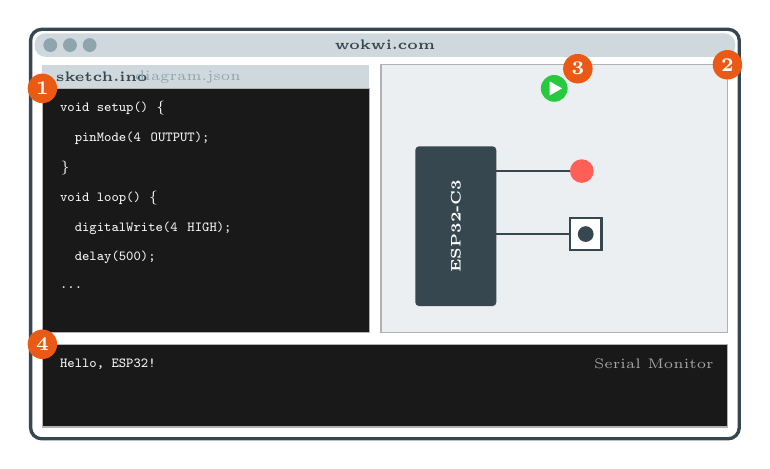
\begin{tikzpicture}[font=\tiny]
    \draw[nInk, very thick, fill=white, rounded corners=4pt] (0,0) rectangle (9,5.2);
    \fill[nLight, rounded corners=4pt] (0.05,4.85) rectangle (8.95,5.15);
    \fill[nLine] (0.25,5.0) circle (2.5pt); \fill[nLine] (0.5,5.0) circle (2.5pt); \fill[nLine] (0.75,5.0) circle (2.5pt);
    \node[font=\tiny\bfseries, text=nInk] at (4.5,5.0) {wokwi.com};
    % code editor
    \fill[nLight] (0.15,4.45) rectangle (4.3,4.75);
    \node[anchor=west, font=\tiny\bfseries, text=nInk] at (0.2,4.6) {sketch.ino};
    \node[anchor=west, font=\tiny, text=nLine] at (1.2,4.6) {diagram.json};
    \draw[gray!60, fill=VSDarkBg] (0.15,1.35) rectangle (4.3,4.45);
    \foreach \t [count=\j from 0] in {void setup() \{, \ \ pinMode(4\, OUTPUT);, \}, void loop() \{, \ \ digitalWrite(4\, HIGH);, \ \ delay(500);, \ldots}
      \node[anchor=west, text=VSText, font=\ttfamily\tiny] at (0.25,{4.2-0.38*\j}) {\t};
    % diagram
    \draw[gray!60, fill=nFill] (4.45,1.35) rectangle (8.85,4.75);
    \fill[MacGreen] (6.65,4.45) circle (0.17);
    \fill[white] (6.59,4.36) -- (6.59,4.54) -- (6.75,4.45) -- cycle;
    \draw[nInk, thick, fill=nInk, rounded corners=1pt] (4.9,1.7) rectangle (5.9,3.7);
    \node[font=\tiny\bfseries, text=white, rotate=90] at (5.4,2.7) {ESP32-C3};
    \fill[MacRed] (7.0,3.4) circle (0.15);
    \draw[nInk, thick] (5.9,3.4) -- (6.85,3.4);
    \draw[nInk, thick, fill=white] (6.85,2.4) rectangle (7.25,2.8);
    \fill[nInk] (7.05,2.6) circle (0.1);
    \draw[nInk, thick] (5.9,2.6) -- (6.85,2.6);
    % serial monitor
    \draw[gray!60, fill=VSDarkBg] (0.15,0.15) rectangle (8.85,1.2);
    \node[anchor=west, text=VSText, font=\ttfamily\tiny] at (0.25,0.95) {Hello, ESP32!};
    \node[anchor=east, font=\tiny, text=gray!70] at (8.8,0.95) {Serial Monitor};
    % badges
    \foreach \x/\y/\n in {0.15/4.45/1, 8.85/4.75/2, 6.95/4.7/3, 0.15/1.2/4}
      \node[circle, fill=AccentOrange, text=white, font=\bfseries\scriptsize, inner sep=1.5pt] at (\x,\y) {\n};
  \end{tikzpicture}}

% ---------- our circuit for today ----------
\newcommand{\ourcircuit}{%
  \begin{tikzpicture}[>=Stealth, font=\scriptsize]
    \node[draw=nInk, very thick, fill=nInk, text=white, rounded corners=3pt, minimum width=2.0cm,
      minimum height=3.2cm, font=\scriptsize\bfseries, align=center] (esp) at (0,0) {ESP32-C3};
    \node[lbox, draw=nLine, fill=nFill, text=nInk, minimum width=1.9cm] (led) at (4.2,1.2) {\faLightbulb\ LED};
    \node[lbox, draw=nInk, fill=nFill, minimum width=1.9cm] (ba) at (4.2,0.4) {\faDotCircle\ Button A};
    \node[lbox, draw=nInk, fill=nFill, minimum width=1.9cm] (bb) at (4.2,-0.4) {\faDotCircle\ Button B};
    \node[lbox, draw=nLine, fill=nFill, text=nInk, minimum width=1.9cm] (lcd) at (4.2,-1.25) {\faTv\ LCD 16$\times$2};
    \draw[very thick, nInk] (esp.east |- led) -- node[above, font=\tiny] {GPIO 4} (led);
    \draw[very thick, nInk] (esp.east |- ba) -- node[above, font=\tiny] {GPIO 5} (ba);
    \draw[very thick, nInk] (esp.east |- bb) -- node[above, font=\tiny] {GPIO 6} (bb);
    \draw[very thick, nInk] (esp.east |- lcd) -- node[above, font=\tiny] {GPIO 8, 9 (I2C)} (lcd);
  \end{tikzpicture}}

% ---------- Wokwi-style parts for the "Build it" slides ----------
\definecolor{PcbBlack}{RGB}{38,38,40}
\definecolor{ResBody}{RGB}{214,184,140}
\definecolor{LcdScreen}{RGB}{131,190,40}
\definecolor{WireGreen}{RGB}{0,140,40}
\newcommand{\pinfont}{\fontsize{3.4}{3.6}\selectfont}
\tikzset{
  % a wire; the white edge makes crossings easy to see
  wire/.style={line width=1.1pt, rounded corners=1.5pt, preaction={draw, white, line width=2.6pt}},
  % ESP32-C3-DevKitM-1 as in Wokwi (USB at the bottom); pins (-L0)..(-L14), (-R0)..(-R14), 0 = top
  pics/esp32c3/.style={code={
    \fill[PcbBlack, rounded corners=2pt] (0,0) rectangle (2.7,4.9);
    % module ESP32-C3-MINI-1: the antenna part sticks out above the board
    \fill[gray!55, rounded corners=0.8pt] (0.62,2.95) rectangle (2.08,5.3);
    \draw[white, line width=0.5pt] (0.72,4.85) -- (0.72,5.18)
      \foreach \i in {1,...,3} { -- ++(0.2,0) -- ++(0,-0.26) -- ++(0.2,0) -- ++(0,0.26) } -- ++(0.1,0);
    \fill[gray!22, rounded corners=0.5pt] (0.66,2.99) rectangle (2.04,4.72);
    \draw[gray!55, line width=0.7pt] (1.35,3.85) circle (0.22);
    \draw[gray!55, line width=0.5pt] (1.26,3.77) arc (180:90:0.13) (1.19,3.77) arc (180:90:0.21);
    \node[font=\pinfont, text=gray!55!black] at (1.35,3.3) {ESP32-C3-MINI-1};
    % voltage regulator: 3 small legs on the left, a wide tab on the right
    \foreach \y in {2.14,2.28,2.42} \fill[gray!65] (0.66,\y-0.03) rectangle (0.76,\y+0.03);
    \fill[gray!65] (1.18,2.16) rectangle (1.3,2.4);
    \fill[black] (0.76,2.07) rectangle (1.2,2.49);
    % RGB LED on GPIO 8
    \fill[gray!10] (1.75,2.12) rectangle (2.05,2.42);
    \fill[white] (1.8,2.17) rectangle (2.0,2.37);
    \node[font=\pinfont\bfseries\rmfamily, text=white] at (1.9,2.58) {GPIO8};
    % USB-to-serial chip with pins on all sides
    \foreach \i in {0,...,4} {
      \fill[gray!65] ({1.34+0.1*\i},1.16) rectangle ++(0.04,0.05);
      \fill[gray!65] ({1.34+0.1*\i},1.69) rectangle ++(0.04,0.05);
      \fill[gray!65] (1.26,{1.24+0.1*\i}) rectangle ++(0.05,0.04);
      \fill[gray!65] (1.79,{1.24+0.1*\i}) rectangle ++(0.05,0.04);
    }
    \fill[black] (1.3,1.2) rectangle (1.8,1.7);
    % power LED
    \fill[MacRed] (0.72,1.28) rectangle (0.84,1.44);
    % BOOT and RST buttons
    \foreach \x/\t in {0.75/BOOT,1.95/RST} {
      \fill[gray!15] (\x-0.18,0.35) rectangle (\x+0.18,0.71);
      \fill[black!85] (\x,0.53) circle (0.12);
      \node[font=\pinfont\bfseries\rmfamily, text=white] at (\x,0.86) {\t};
    }
    % USB connector, sticks out below the board
    \fill[gray!55] (1.05,-0.14) rectangle (1.65,0.42);
    \fill[gray!30] (1.12,-0.14) rectangle (1.58,0.3);
    \foreach \n [count=\k from 0] in {GND,3V3,3V3,2,3,GND,RST,GND,0,1,10,GND,5V,5V,GND} {
      \fill[MacYellow] (0.15,{4.5-0.3*\k}) circle (0.065);
      \node[rotate=90, font=\pinfont, text=white] at (0.34,{4.5-0.3*\k}) {\n};
      \coordinate (-L\k) at (0.15,{4.5-0.3*\k});
    }
    \foreach \n [count=\k from 0] in {GND,TX,RX,GND,9,8,GND,7,6,5,4,GND,18,19,GND} {
      \fill[MacYellow] (2.55,{4.5-0.3*\k}) circle (0.065);
      \node[rotate=90, font=\pinfont, text=white] at (2.36,{4.5-0.3*\k}) {\n};
      \coordinate (-R\k) at (2.55,{4.5-0.3*\k});
    }
  }},
  % red LED, origin = middle of the rim; legs (-C) straight, (-A) bent
  pics/wled/.style={code={
    \draw[gray!60, line width=0.9pt] (-0.09,0) -- (-0.09,-0.42);
    \draw[gray!60, line width=0.9pt] (0.09,0) -- (0.09,-0.12) -- (0.17,-0.2) -- (0.17,-0.42);
    \fill[MacRed!80!black] (-0.24,0) rectangle (0.24,0.07);
    \fill[MacRed] (-0.2,0.07) -- (-0.2,0.32) arc (180:0:0.2) -- (0.2,0.07) -- cycle;
    \fill[white, opacity=0.45] (-0.1,0.38) ellipse (0.04 and 0.1);
    \node[font=\pinfont, text=black, anchor=east] at (-0.1,-0.3) {C};
    \node[font=\pinfont, text=black, anchor=west] at (0.18,-0.3) {A};
    \coordinate (-C) at (-0.09,-0.42);
    \coordinate (-A) at (0.17,-0.42);
  }},
  % 220 ohm resistor, vertical; origin = bottom lead (-2), top lead (-1)
  pics/wres/.style={code={
    \draw[gray!60, line width=0.9pt] (0,0) -- (0,0.85);
    \fill[ResBody, rounded corners=0.8pt] (-0.09,0.15) rectangle (0.09,0.7);
    \foreach \y/\c in {0.6/red, 0.52/red, 0.44/brown!80!black, 0.24/MacYellow!70!brown}
      \fill[\c] (-0.09,\y) rectangle (0.09,\y+0.05);
    \coordinate (-1) at (0,0.85);
    \coordinate (-2) at (0,0);
  }},
  % pushbutton, origin = centre; legs (-1l), (-2l), (-1r), (-2r); argument = colour of the cap
  pics/wbutton/.style={code={
    \foreach \x in {-1,1} \foreach \y in {-1,1}
      \draw[gray!60, line width=0.9pt] (0.3*\x,0.13*\y) -- (0.4*\x,0.13*\y);
    \fill[black!80, rounded corners=1pt] (-0.3,-0.25) rectangle (0.3,0.25);
    \fill[gray!35] (-0.25,-0.2) rectangle (0.25,0.2);
    \fill[#1] (0,0) circle (0.14);
    \node[font=\pinfont, text=black, anchor=south east] at (-0.33,0.13) {1.l};
    \node[font=\pinfont, text=black, anchor=north west] at (0.33,-0.13) {2.r};
    \node[font=\pinfont, text=black, anchor=north east] at (-0.33,-0.13) {2.l};
    \node[font=\pinfont, text=black, anchor=south west] at (0.33,0.13) {1.r};
    \coordinate (-1l) at (-0.4,0.13);  \coordinate (-2l) at (-0.4,-0.13);
    \coordinate (-1r) at (0.4,0.13);   \coordinate (-2r) at (0.4,-0.13);
  }},
  % LCD 16x2 with I2C, origin = bottom left; pins (-GND), (-VCC), (-SDA), (-SCL) on the left edge
  pics/wlcd/.style={code={
    \fill[mygreen!55!black, rounded corners=1.5pt] (0,0) rectangle (3.0,1.2);
    \fill[black!85] (0.55,0.12) rectangle (2.9,1.08);
    \fill[LcdScreen] (0.62,0.2) rectangle (2.83,1.0);
    \foreach \r in {0,1} \foreach \c in {0,...,15}
      \fill[LcdScreen!85!black] ({0.66+0.135*\c},{0.26+0.38*\r}) rectangle ++(0.11,0.3);
    \foreach \n [count=\k from 0] in {GND,VCC,SDA,SCL} {
      \fill[MacYellow] (0.14,{1.0-0.2*\k}) circle (0.055);
      \node[font=\pinfont, text=white, anchor=west] at (0.2,{1.0-0.2*\k}) {\n};
      \coordinate (-\n) at (0.14,{1.0-0.2*\k});
    }
  }},
}

% the circuit of the day, built in 4 steps: #1 = step (1 LED, 2 button A, 3 LCD, 4 button B)
% parts of the current step are drawn normally, parts of earlier steps are faded
\newcommand{\buildopacity}[2]{\ifnum#1>#2 0.3\else 1\fi}
\newcommand{\buildpic}[1]{%
  \begin{tikzpicture}[font=\tiny]
    \useasboundingbox (-0.45,-0.2) rectangle (7.3,5.7);
    \pic (esp) at (0,0) {esp32c3};
    % step 1: LED and resistor, GND along the bottom
    \begin{scope}[opacity=\buildopacity{#1}{1}]
      \pic (res) at (4.91,0.65) {wres};
      \pic (led) at (5.0,1.95) {wled};
      \draw[wire, black] (esp-R14) -- (4.91,0.3) -- (res-2);
      \draw[wire, WireGreen] (res-1) -- (led-C);
      \draw[wire, WireGreen] (esp-R10) -| (4.25,0.48) -| (led-A);
      \node[font=\fontsize{5.5}{6}\selectfont\bfseries, anchor=east] at (4.83,1.05) {220\,$\Omega$};
    \end{scope}
    % step 2: button A
    \ifnum#1>1
    \begin{scope}[opacity=\buildopacity{#1}{2}]
      \pic (ba) at (4.9,2.85) {wbutton=MacGreen};
      \node[font=\scriptsize\bfseries, anchor=south] at (4.9,3.1) {A};
      \draw[wire, black] (ba-2r) -| (5.75,0.3) -- (4.91,0.3);
      \draw[wire, WireGreen] (esp-R9) -| ([xshift=-0.35cm]ba-1l) -- (ba-1l);
    \end{scope}
    \fi
    % step 3: LCD (I2C)
    \ifnum#1>2
    \begin{scope}[opacity=\buildopacity{#1}{3}]
      \pic (lcd) at (4.2,4.2) {wlcd};
      \draw[wire, black] (esp-R0) -| ([xshift=-1.09cm]lcd-GND) -- (lcd-GND);
      \draw[wire, StorageBlue] (esp-R5) -| ([xshift=-0.59cm]lcd-SDA) -- (lcd-SDA);
      \draw[wire, ProgramPurple] (esp-R4) -| ([xshift=-0.79cm]lcd-SCL) -- (lcd-SCL);
      \draw[wire, MacRed] (esp-L12) -- (-0.35,0.9) -- (-0.35,5.6) -- (4.0,5.6) |- (lcd-VCC);
    \end{scope}
    \fi
    % step 4: button B
    \ifnum#1>3
    \begin{scope}[opacity=\buildopacity{#1}{4}]
      \pic (bb) at (4.9,3.75) {wbutton=StorageBlue};
      \node[font=\scriptsize\bfseries, anchor=south] at (4.9,4.0) {B};
      \draw[wire, black] (bb-2r) -| (5.75,2.72);
      \fill (5.75,2.72) circle (0.05);
      \draw[wire, WireGreen] (esp-R8) -| ([xshift=-0.55cm]bb-1l) -- (bb-1l);
    \end{scope}
    \fi
  \end{tikzpicture}}

% ---------- the robot of Task 3 (the parts as in Wokwi, the wires as thick buses) ----------
\definecolor{SonarBlue}{RGB}{20,90,160}
\definecolor{DriverGreen}{RGB}{20,130,70}
\tikzset{
  % HC-SR04 distance sensor, origin = bottom left, 2.6 x 1.1
  pics/wsonar/.style={code={
    \fill[SonarBlue, rounded corners=1.5pt] (0,0) rectangle (2.6,1.1);
    \foreach \x in {0.58,2.02} {
      \fill[gray!45] (\x,0.55) circle (0.43);
      \fill[black!70] (\x,0.55) circle (0.33);
      \foreach \r in {0.08,0.16,0.24} \draw[gray!60, line width=0.3pt] (\x,0.55) circle (\r);
    }
    \fill[gray!70, rounded corners=0.5pt] (1.15,0.62) rectangle (1.45,0.78);
    \node[font=\pinfont\bfseries, text=white] at (1.3,0.95) {HC-SR04};
    \foreach \x in {0.95,1.15,1.45,1.65} \fill[MacYellow] (\x,0.1) circle (0.04);
  }},
  % A4988 stepper driver, origin = bottom left, 0.9 x 1.1
  pics/wdriver/.style={code={
    \fill[DriverGreen, rounded corners=1pt] (0,0) rectangle (0.9,1.1);
    \fill[black!85] (0.27,0.3) rectangle (0.63,0.66);
    \node[font=\pinfont\bfseries, text=white] at (0.45,0.88) {A4988};
    \foreach \y in {0.15,0.3,...,0.96} { \fill[MacYellow] (0.08,\y) circle (0.03); \fill[MacYellow] (0.82,\y) circle (0.03); }
  }},
  % stepper motor (NEMA 17) seen from the front, origin = centre; the orange arrow shows its position
  pics/wstepper/.style={code={
    \fill[gray!35, rounded corners=3pt] (-0.8,-0.8) rectangle (0.8,0.8);
    \foreach \x in {-1,1} \foreach \y in {-1,1} \fill[gray!60] (0.62*\x,0.62*\y) circle (0.07);
    \fill[gray!55] (0,0) circle (0.5);
    \fill[gray!25] (0,0) circle (0.3);
    \draw[AccentOrange, line width=2pt, -{Stealth[length=4pt]}] (0,0) -- (40:0.55);
    \fill[gray!80] (0,0) circle (0.1);
  }},
  % buzzer, origin = centre
  pics/wbuzzer/.style={code={
    \fill[black!85] (0,0) circle (0.38);
    \draw[gray!60, line width=0.4pt] (0,0) circle (0.25);
    \fill[gray!40] (0,0) circle (0.07);
  }},
  bus/.style={line width=2.4pt, gray!55},
  buslabel/.style={font=\tiny, text=black, fill=white, inner sep=0.6pt},
  partlabel/.style={font=\small\bfseries, text=nInk},
}
\newcommand{\robotpic}{%
  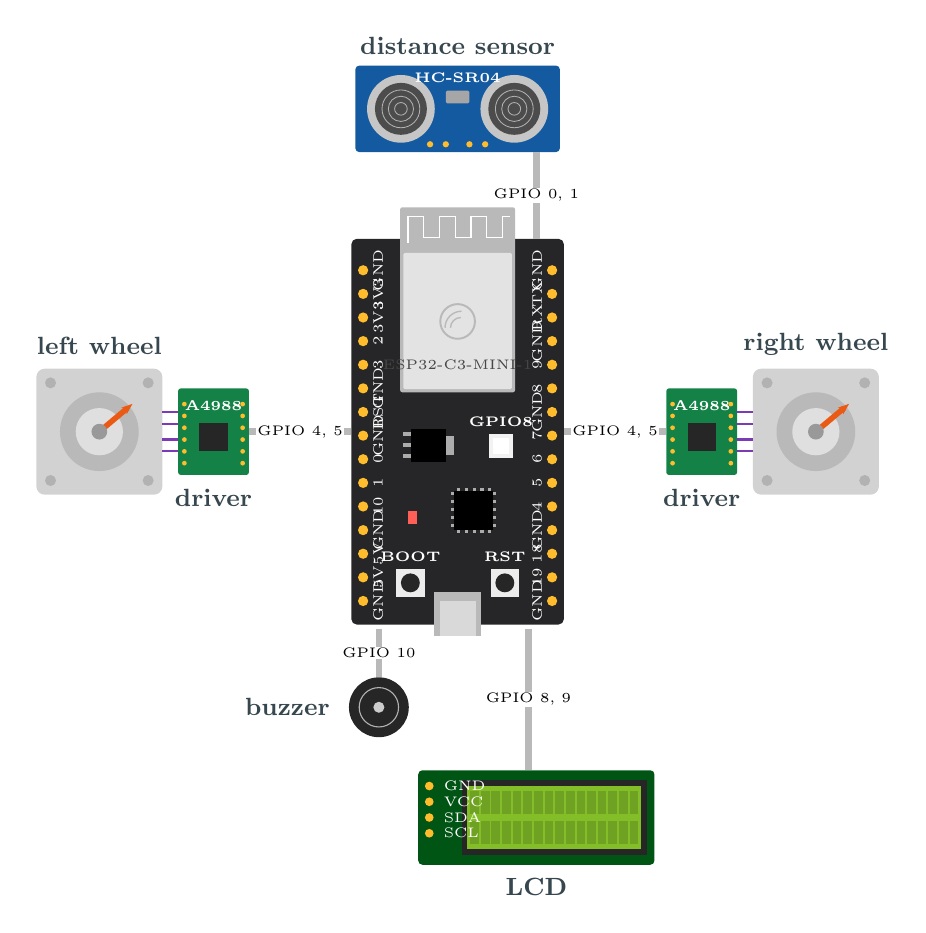
\begin{tikzpicture}
    \pic (esp) at (0,0) {esp32c3};
    % distance sensor, above the board
    \pic at (0.05,6.0) {wsonar};
    \node[partlabel, anchor=south] at (1.35,7.12) {distance sensor};
    \draw[bus] (2.35,4.9) -- (2.35,6.0) node[buslabel, midway] {GPIO 0, 1};
    % wheels: a driver and a stepper motor on each side
    \foreach \s/\dx/\mx/\t in {1/4.0/5.9/right wheel, -1/-2.2/-3.2/left wheel} {
      \pic at (\dx,1.9) {wdriver};
      \pic at (\mx,2.45) {wstepper};
      \node[partlabel, anchor=south] at (\mx,3.3) {\t};
      \node[partlabel, anchor=north] at ({\dx+0.45},1.85) {driver};
      \foreach \y in {2.2,2.35,2.55,2.7}
        \draw[ProgramPurple, line width=0.8pt] ({\dx+0.45+0.45*\s},\y) -- ({\mx-0.8*\s},\y);
    }
    \draw[bus] (2.7,2.45) -- (4.0,2.45) node[buslabel, midway] {GPIO 4, 5};
    \draw[bus] (0,2.45) -- (-1.3,2.45) node[buslabel, midway] {GPIO 4, 5};
    % buzzer and LCD, below the board
    \pic at (0.35,-1.05) {wbuzzer};
    \node[partlabel, anchor=east] at (-0.15,-1.05) {buzzer};
    \draw[bus] (0.35,-0.05) -- (0.35,-0.67) node[buslabel, midway] {GPIO 10};
    \pic at (0.85,-3.05) {wlcd};
    \node[partlabel, anchor=north] at (2.35,-3.1) {LCD};
    \draw[bus] (2.25,-0.05) -- (2.25,-1.85) node[buslabel, midway] {GPIO 8, 9};
  \end{tikzpicture}}

% ---------- power: VCC, GND and a closed loop ----------
\newcommand{\powerexplain}{%
  \begin{tikzpicture}[font=\scriptsize, >=Stealth]
    % rails
    \draw[line width=2pt, nInk] (0,2.0) -- (4.6,2.0);
    \node[anchor=west, font=\scriptsize\bfseries, text=nInk, align=left] at (4.7,2.0) {VCC (+)\\[-1pt]{\tiny 3V3 = 3.3\,V, 5V = 5\,V}};
    \draw[line width=2pt, black] (0,-1.0) -- (4.6,-1.0);
    \node[anchor=west, font=\scriptsize\bfseries, align=left] at (4.7,-1.0) {GND ($-$)\\[-1pt]{\tiny 0\,V}};
    % voltage between the rails
    \draw[<->, thick, DeepBlue] (-0.4,-1.0) -- node[left, font=\scriptsize\bfseries, align=center] {voltage\\3.3\,V} (-0.4,2.0);
    % a part between the rails: resistor + LED
    \draw[thick] (1.2,2.0) -- (1.2,1.55);
    \draw[thick, fill=ResBody] (1.08,1.55) rectangle (1.32,0.85);
    \draw[thick] (1.2,0.85) -- (1.2,0.6);
    \draw[thick, fill=nFill] (0.95,0.6) -- (1.45,0.6) -- (1.2,0.15) -- cycle;
    \draw[very thick] (0.95,0.15) -- (1.45,0.15);
    \foreach \d in {0,0.15} \draw[->, nInk, thick] (1.5,{0.45-\d}) -- ++(0.28,0.16);
    \draw[thick] (1.2,0.15) -- (1.2,-1.0);
    \fill[nInk] (1.2,2.0) circle (0.06);  \fill (1.2,-1.0) circle (0.06);
    \draw[->, line width=1.4pt, AccentOrange] (0.65,1.8) -- node[sloped, above, font=\tiny\bfseries] {current} (0.65,-0.8);
    \node[font=\tiny\bfseries, aExec, align=center] at (1.2,-1.4) {\faCheck\ closed loop:\\+ $\to$ part $\to$ GND};
    % a short circuit
    \draw[line width=1.4pt, aWrite] (3.6,2.0) -- (3.6,-1.0);
    \fill[nInk] (3.6,2.0) circle (0.06);  \fill (3.6,-1.0) circle (0.06);
    \node[font=\Large\bfseries, text=aWrite, fill=white, inner sep=1pt] at (3.6,0.5) {\faTimes};
    \node[font=\tiny\bfseries, aWrite, align=center] at (3.6,-1.4) {\faTimes\ short circuit:\\VCC straight to GND};
  \end{tikzpicture}}

% ---------- how an LED works: the part and its circuit ----------
\newcommand{\ledexplain}{%
  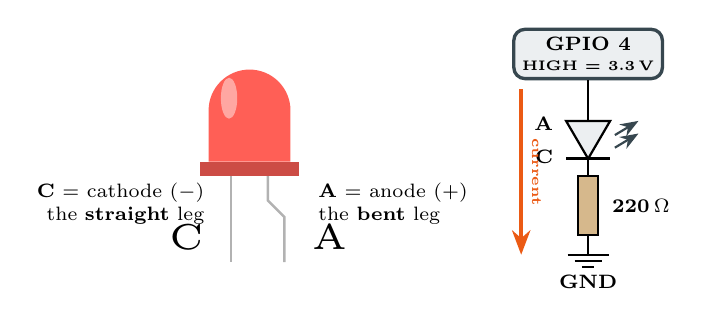
\begin{tikzpicture}[font=\scriptsize, >=Stealth]
    \begin{scope}[scale=2.6, transform shape]
      \pic (bl) at (0,0) {wled};
    \end{scope}
    \node[anchor=west, align=left] (la) at (0.75,-0.35) {\textbf{A} = anode (+)\\the \textbf{bent} leg};
    \node[anchor=east, align=right] (lc) at (-0.45,-0.35) {\textbf{C} = cathode ($-$)\\the \textbf{straight} leg};
    % the circuit
    \begin{scope}[xshift=4.3cm, yshift=-0.2cm]
      \node[lbox, draw=nInk, fill=nFill] (gpio) at (0,1.75) {GPIO 4\\[-1pt]{\tiny HIGH = 3.3\,V}};
      \draw[thick] (gpio.south) -- (0,0.9);
      \draw[thick, fill=nFill] (-0.28,0.9) -- (0.28,0.9) -- (0,0.42) -- cycle;
      \draw[very thick] (-0.28,0.42) -- (0.28,0.42);
      \foreach \d in {0,0.16} \draw[->, nInk, thick] (0.34,{0.72-\d}) -- ++(0.3,0.18);
      \node[anchor=east, font=\scriptsize\bfseries] at (-0.32,0.86) {A};
      \node[anchor=east, font=\scriptsize\bfseries] at (-0.32,0.44) {C};
      \draw[thick] (0,0.42) -- (0,0.2);
      \draw[thick, fill=ResBody] (-0.13,0.2) rectangle (0.13,-0.55);
      \node[anchor=west, font=\scriptsize\bfseries] at (0.18,-0.18) {220\,$\Omega$};
      \draw[thick] (0,-0.55) -- (0,-0.8);
      \foreach \w/\y in {0.26/-0.8, 0.17/-0.88, 0.08/-0.96} \draw[thick] (-\w,\y) -- (\w,\y);
      \node[font=\scriptsize\bfseries] at (0,-1.15) {GND};
      \draw[->, line width=1.3pt, AccentOrange] (-0.85,1.3) -- node[sloped, above, font=\tiny\bfseries] {current} (-0.85,-0.8);
    \end{scope}
  \end{tikzpicture}}

% ---------- how a pushbutton works: 4 legs, 2 pairs ----------
% #1 = 0 not pressed, 1 pressed
\newcommand{\buttoninside}[1]{%
  \begin{tikzpicture}[font=\tiny, >=Stealth]
    \foreach \x/\y/\n in {0/0.8/1.l, 1.6/0.8/1.r, 0/0/2.l, 1.6/0/2.r} {
      \fill[gray!60] (\x,\y) circle (0.06);
      \node[font=\tiny\bfseries, anchor=\ifdim\x pt<1pt east\else west\fi] at (\x,\y) {\n};
    }
    \draw[thick] (0,0.8) -- (1.6,0.8);
    \draw[thick] (0,0) -- (1.6,0);
    \fill (0.8,0.8) circle (0.04);  \fill (0.8,0) circle (0.04);
    \ifnum#1=0
      \draw[thick] (0.8,0.8) -- (0.8,0.62) -- (1.1,0.22);
      \draw[thick] (0.8,0) -- (0.8,0.18);
    \else
      \draw[line width=1.6pt, nInk] (0.8,0.8) -- (0.8,0);
    \fi
  \end{tikzpicture}}
\newcommand{\buttonexplain}{%
  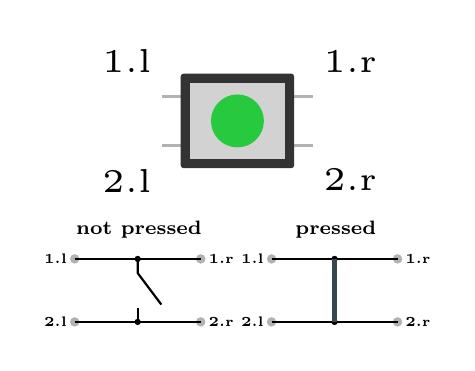
\begin{tikzpicture}[font=\scriptsize]
    \begin{scope}[scale=2.4, transform shape]
      \pic (bx) at (0,0) {wbutton=MacGreen};
    \end{scope}
    \node[anchor=north, align=center] at (-1.25,-1.15) {\textbf{not pressed}\\[2pt]\buttoninside{0}};
    \node[anchor=north, align=center] at (1.25,-1.15) {\textbf{pressed}\\[2pt]\buttoninside{1}};
  \end{tikzpicture}}

% ---------- I2C: one controller, many devices on 2 wires ----------
\newcommand{\itwocbus}{%
  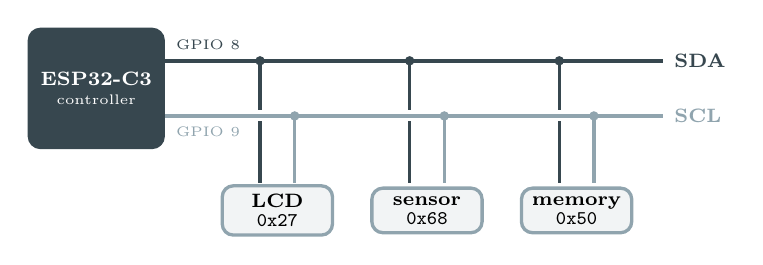
\begin{tikzpicture}[font=\scriptsize, >=Stealth]
    \node[lbox, draw=nInk, fill=nInk, text=white, minimum width=1.7cm, minimum height=1.5cm]
      (cpu) at (0,0) {ESP32-C3\\[-1pt]{\tiny\mdseries controller}};
    \draw[line width=1.5pt, nInk] (cpu.east |- 0,0.35) node[above right, font=\tiny] {GPIO 8} -- (7.2,0.35)
      node[right, font=\scriptsize\bfseries] {SDA};
    \foreach \x/\n/\a/\c in {2.3/LCD/0x27/nLine, 4.2/sensor/0x68/nLine, 6.1/memory/0x50/nLine} {
      \draw[line width=1.2pt, nInk] (\x-0.22,0.35) -- (\x-0.22,-1.2);
      \fill[nInk] (\x-0.22,0.35) circle (0.06);
      \node[lbox, draw=\c, fill=\c!12, minimum width=1.4cm] at (\x,-1.55) {\n\\[-1pt]\texttt{\a}};
    }
    \draw[line width=1.5pt, nLine, preaction={draw, white, line width=4pt}] (cpu.east |- 0,-0.35)
      node[below right, font=\tiny] {GPIO 9} -- (7.2,-0.35) node[right, font=\scriptsize\bfseries] {SCL};
    \foreach \x in {2.3,4.2,6.1} {
      \draw[line width=1.2pt, nLine] (\x+0.22,-0.35) -- (\x+0.22,-1.2);
      \fill[nLine] (\x+0.22,-0.35) circle (0.06);
    }
  \end{tikzpicture}}

% ---------- one I2C message on the wires: #1 = the step to highlight (1..6) ----------
\newcommand{\itwoctiming}[1]{%
  \begin{tikzpicture}[font=\scriptsize, >=Stealth]
    % the steps: highlighted band and a label on top
    \foreach \n/\a/\b/\t/\c in {1/0.3/1.0/START/AccentOrange, 2/1.0/5.0/{address \texttt{0x27} + write}/AccentOrange,
        3/5.0/5.5/ACK/AccentOrange, 4/5.5/9.5/{data byte}/AccentOrange, 5/9.5/10.0/ACK/AccentOrange, 6/10.0/10.75/STOP/AccentOrange} {
      \ifnum\n=#1
        \fill[\c!18, rounded corners=2pt] (\a,-1.55) rectangle (\b,1.45);
        \node[font=\scriptsize\bfseries, text=\c!80!black] at ({(\a+\b)/2},1.25) {\t};
      \else
        \node[font=\tiny, text=gray] at ({(\a+\b)/2},1.25) {\t};
      \fi
      \draw[gray!40, densely dotted] (\a,-1.55) -- (\a,1.1);
    }
    \node[anchor=east, font=\scriptsize\bfseries, text=nInk] at (-0.1,0.6) {SCL};
    \node[anchor=east, font=\scriptsize\bfseries, text=nInk] at (-0.1,-0.6) {SDA};
    % SCL: high, falls after START, 18 clock ticks, high again before STOP
    \draw[thick, nInk] (0,0.9) -- (0.8,0.9) -- (0.8,0.3) -- (1.25,0.3)
      \foreach \k in {0,...,17} { -- ({1.25+0.5*\k},0.9) -- ({1.5+0.5*\k},0.9) -- ({1.5+0.5*\k},0.3) -- ({1.75+0.5*\k},0.3) }
      -- (10.2,0.3) -- (10.2,0.9) -- (10.9,0.9);
    % SDA: falls at START, one bit per tick, rises at STOP
    \draw[thick, nInk] (0,-0.3) -- (0.5,-0.3) -- (0.5,-0.9) -- (1.0,-0.9);
    \foreach \x/\p/\v/\c in {1.0/0/0/nInk, 1.5/0/1/nInk, 2.0/1/0/nInk, 2.5/0/0/nInk, 3.0/0/1/nInk, 3.5/1/1/nInk, 4.0/1/1/nInk, 4.5/1/0/nInk, 5.0/0/0/nInk, 5.5/0/0/nInk, 6.0/0/1/nInk, 6.5/1/0/nInk, 7.0/0/0/nInk, 7.5/0/1/nInk, 8.0/1/0/nInk, 8.5/0/0/nInk, 9.0/0/0/nInk, 9.5/0/0/nInk}
      \draw[thick, \c] (\x,{-0.9+0.6*\p}) -- (\x,{-0.9+0.6*\v}) -- (\x+0.5,{-0.9+0.6*\v});
    \draw[thick, nInk] (10.0,-0.9) -- (10.45,-0.9) -- (10.45,-0.3) -- (10.9,-0.3);
    \foreach \x/\v in {1.25/0, 1.75/1, 2.25/0, 2.75/0, 3.25/1, 3.75/1, 4.25/1, 4.75/0, 5.25/0, 5.75/0, 6.25/1, 6.75/0, 7.25/0, 7.75/1, 8.25/0, 8.75/0, 9.25/0, 9.75/0} \node[font=\tiny, text=gray!70!black] at (\x,-1.2) {\v};
    \node[font=\tiny, text=gray!70!black] at (4.75,-1.42) {W};
  \end{tikzpicture}}

% ---------- showcase: Snake on a Nokia 5110 screen with a joystick ----------
\newcommand{\snakeshowcase}{%
  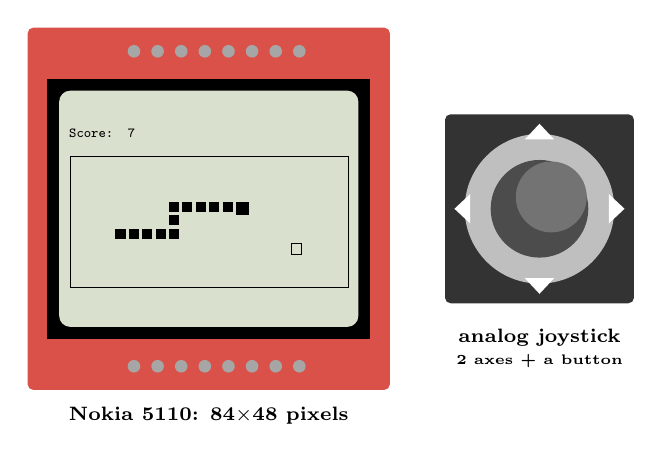
\begin{tikzpicture}[font=\scriptsize]
    % the Nokia 5110 module
    \fill[MacRed!85!black, rounded corners=2pt] (0,0) rectangle (4.6,4.6);
    \foreach \i in {0,...,7} {
      \fill[gray!70] ({1.35+0.3*\i},0.3) circle (0.08);
      \fill[gray!70] ({1.35+0.3*\i},4.3) circle (0.08);
    }
    \fill[black] (0.25,0.65) rectangle (4.35,3.95);
    \fill[LcdScreen!40!gray!30, rounded corners=4pt] (0.4,0.8) rectangle (4.2,3.8);
    % the game: 84 x 48 pixels drawn at 0.0425 cm per pixel
    \begin{scope}[shift={(0.52,3.32)}, x=0.0425cm, y=-0.0425cm]
      \node[anchor=north west, inner sep=0, font=\ttfamily\bfseries\tiny] at (0,0) {Score: 7};
      \draw[line width=0.3pt] (0.5,8.5) rectangle (83.5,47.5);
      \foreach \x/\y in {3/5,4/5,5/5,6/5,7/5,7/4,7/3,8/3,9/3,10/3,11/3} \fill ({2+4*\x},{10+4*\y}) rectangle ++(3,3);
      \fill ({2+4*12},{10+4*3}) rectangle ++(4,4);
      \draw[line width=0.3pt] ({2+4*16+0.5},{10+4*6+0.5}) rectangle ++(3,3);
    \end{scope}
    \node[font=\scriptsize\bfseries, anchor=north] at (2.3,-0.1) {Nokia 5110: 84$\times$48 pixels};
    % the joystick
    \begin{scope}[shift={(5.3,1.1)}]
      \fill[black!80, rounded corners=2pt] (0,0) rectangle (2.4,2.4);
      \fill[gray!50] (1.2,1.2) circle (0.95);
      \fill[black!70] (1.2,1.2) circle (0.62);
      \fill[black!55] (1.35,1.35) circle (0.45);
      \foreach \a in {0,90,180,270} \fill[white] ([shift={(\a:1.08)}]1.2,1.2) -- ([shift={(\a+12:0.9)}]1.2,1.2) -- ([shift={(\a-12:0.9)}]1.2,1.2) -- cycle;
      \node[font=\scriptsize\bfseries, anchor=north, align=center] at (1.2,-0.2) {analog joystick\\{\tiny 2 axes + a button}};
    \end{scope}
  \end{tikzpicture}}

% ---------- inside the ESP32-C3: CPU, internal bus, controllers; pins and wires outside ----------
% #1 = 0 overview, 1 address on the bus, 2 GPIO recognises it, 3 data written: the LED lights up
\newcommand{\chipbus}[1]{%
  \begin{tikzpicture}[>=Stealth, font=\scriptsize]
    % the chip
    \draw[nLine, very thick, dashed, rounded corners=6pt] (-1.3,-1.6) rectangle (11.9,2.5);
    \node[anchor=north west, font=\scriptsize\bfseries, text=nInk] at (-1.2,2.45) {\faMicrochip\ inside the ESP32-C3 chip};
    \node[cpubox, minimum width=1.8cm, minimum height=0.9cm] (cpu) at (0.4,1.45) {CPU};
    % the internal bus
    \ifnum#1>0 \def\buswidth{1.5pt}\else \def\buswidth{2pt}\fi
    \foreach \y/\c/\t in {0.75/nInk/address, 0.45/nLine/data, 0.15/nLight/control} {
      \draw[line width=\buswidth, \c] (0.4,\y) -- (10.4,\y);
      \node[anchor=west, font=\tiny\bfseries, text=\c] at (10.45,\y) {\t};
    }
    \node[font=\tiny\bfseries, text=nInk, anchor=south] at (5.4,0.78) {internal bus};
    \draw[very thick, nInk] (cpu.south) -- (0.4,0.15);
    % memory and controllers
    \node[rambox, minimum width=2.0cm, minimum height=0.85cm] (mem) at (2.9,-0.75) {Memory\\[-1pt]{\tiny\mdseries RAM, flash}};
    \node[iobox, minimum width=2.0cm, minimum height=0.85cm] (gpio) at (6.0,-0.75) {GPIO controller\\[-1pt]{\tiny\mdseries \texttt{0x6000\,4000}}};
    \node[iobox, minimum width=2.0cm, minimum height=0.85cm] (i2c) at (9.1,-0.75) {I2C controller\\[-1pt]{\tiny\mdseries \texttt{0x6001\,3000}}};
    \foreach \n in {mem,gpio,i2c} \draw[very thick, nInk] (\n.north) -- (\n.north |- 0,0.75);
    % every connection reaches all three groups of lines: address, data and control
    \foreach \x in {0.4,2.9,6.0,9.1}
      \foreach \y/\c in {0.75/nInk, 0.45/nLine, 0.15/nLight}
        \fill[\c] (\x,\y) circle (0.075);
    % pins on the edge of the chip, wires on the board
    \foreach \x/\l/\n in {5.6/4/gpio, 6.4/5/gpio, 8.7/8/i2c, 9.5/9/i2c} {
      \draw[thick, gray!70!black] (\x,-1.175) -- (\x,-1.6);
      \fill[MacYellow] (\x-0.09,-1.69) rectangle (\x+0.09,-1.51);
      \node[font=\tiny\bfseries, anchor=west] at (\x+0.08,-1.4) {\l};
    }
    \draw[line width=1.2pt, WireGreen] (5.6,-1.69) -- (5.6,-2.25);
    \draw[line width=1.2pt, WireGreen] (6.4,-1.69) -- (6.4,-2.25);
    \draw[line width=1.2pt, nInk] (8.7,-1.69) -- (8.7,-2.2);
    \draw[line width=1.2pt, nLine] (9.5,-1.69) -- (9.5,-2.2);
    \ifnum#1=3
      \fill[nLight] (5.6,-2.5) circle (0.38);
      \fill[nInk] (5.6,-2.5) circle (0.24);
      \node[font=\tiny\bfseries, text=nInk, anchor=east] at (5.5,-1.95) {3.3\,V};
    \else
      \fill[white] (5.6,-2.5) circle (0.24); \draw[nLine] (5.6,-2.5) circle (0.24);
    \fi
    \node[font=\tiny, anchor=north] at (5.6,-2.78) {LED};
    \fill[black!75, rounded corners=1pt] (6.2,-2.7) rectangle (6.6,-2.3);  \fill[MacGreen] (6.4,-2.5) circle (0.12);
    \node[font=\tiny, anchor=north] at (6.4,-2.78) {button};
    \node[lbox, draw=nLine, fill=nFill, text=nInk, minimum width=1.6cm] (lcd) at (9.1,-2.55) {LCD\\[-1pt]{\tiny\mdseries I2C address \texttt{0x27}}};
    \node[font=\tiny, text=gray!40!black, anchor=west, align=left] at (10.05,-1.95) {SDA, SCL:\\2 wires};
    \node[font=\scriptsize\bfseries, text=gray!40!black, anchor=west] at (-1.2,-2.2) {on the board: real wires};
    % the steps of one store: sw to 0x6000 4008
    \ifnum#1>0
      \node[font=\tiny\ttfamily, fill=white, draw=nInk, rounded corners=1pt, anchor=west] at (1.5,1.45) {sw a4, 8(a5)};
      \node[font=\tiny\bfseries\ttfamily, fill=white, draw=nLine, rounded corners=1pt] at (1.8,0.75) {0x6000\,4008};
    \fi
    \ifnum#1>1
      \draw[line width=1.6pt, AccentOrange, rounded corners=3pt] ([shift={(-0.08,-0.08)}]gpio.south west) rectangle ([shift={(0.08,0.08)}]gpio.north east);
      \node[font=\tiny\bfseries, text=AccentOrange, anchor=south west] at ([xshift=0.05cm]gpio.north east) {mine!};
      \node[font=\tiny, text=gray, anchor=south west] at ([xshift=0.05cm]mem.north east) {not mine};
      \node[font=\tiny, text=gray, anchor=south west] at ([xshift=0.05cm]i2c.north east) {not mine};
    \fi
    \ifnum#1>2
      \node[font=\tiny\bfseries\ttfamily, fill=white, draw=nLine, rounded corners=1pt] at (1.8,0.45) {0x10 = bit 4};
      \node[font=\tiny\bfseries, fill=white, awrite, rounded corners=1pt] at (1.8,0.15) {write};
    \fi
  \end{tikzpicture}}

% ---------- lcd.print: CPU -> I2C controller (internal bus) -> LCD (2 wires) ----------
\newcommand{\twobuses}{%
  \begin{tikzpicture}[>=Stealth, font=\scriptsize]
    \draw[nLine, very thick, dashed, rounded corners=6pt] (-0.3,-0.75) rectangle (5.3,1.2);
    \node[anchor=north west, font=\tiny\bfseries, text=nInk] at (-0.25,1.17) {\faMicrochip\ inside the chip};
    \node[cpubox, minimum width=1.4cm, minimum height=0.8cm] (cpu) at (0.6,0.1) {CPU};
    \node[iobox, minimum width=1.8cm, minimum height=0.8cm] (ctl) at (4.1,0.1) {I2C\\[-1pt]controller};
    \draw[->, line width=1.8pt, nInk] (cpu.east) -- node[above, font=\tiny\bfseries] {internal bus} node[below, font=\tiny\ttfamily] {sw \ldots\ 0x6001\,3xxx} (ctl.west);
    \node[lbox, draw=nLine, fill=nFill, text=nInk, minimum width=1.4cm, minimum height=0.8cm] (lcd) at (7.3,0.1) {LCD\\[-1pt]{\tiny\mdseries \texttt{0x27}}};
    \draw[->, line width=1.2pt, nInk] ([yshift=0.12cm]ctl.east) -- ([yshift=0.12cm]lcd.west);
    \draw[line width=1.2pt, nLine] ([yshift=-0.12cm]ctl.east) -- ([yshift=-0.12cm]lcd.west);
    \node[font=\tiny\bfseries, anchor=south] at (6.05,0.25) {SDA, SCL};
    \node[font=\tiny, anchor=north, align=center] at (6.05,-0.05) {START, \texttt{0x27},\\data, STOP};
    \node[font=\tiny\bfseries, text=gray!40!black] at (6.05,-0.95) {on the board};
    \node[font=\tiny\ttfamily, anchor=north] at (0.6,-0.32) {lcd.print("K")};
  \end{tikzpicture}}

% ---------- memory-mapped I/O: one address space, the device part zoomed in ----------
\newcommand{\mmiomap}{%
  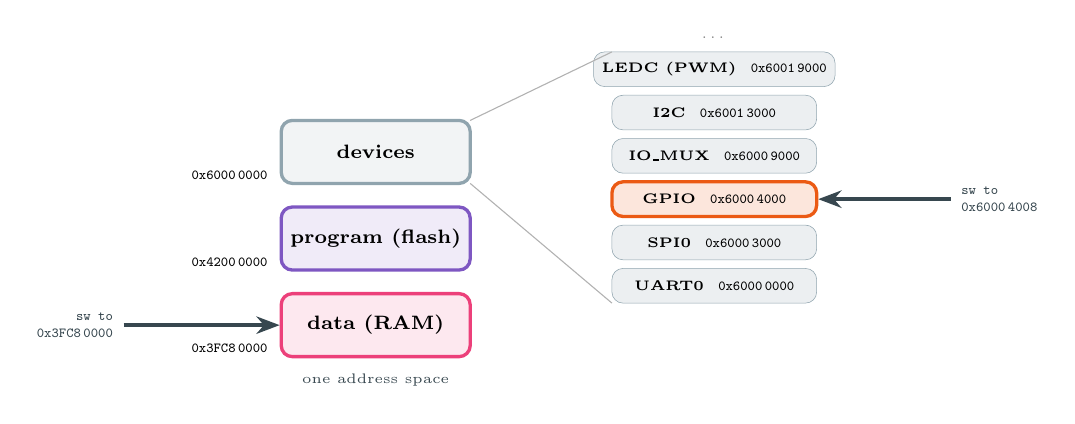
\begin{tikzpicture}[>=Stealth, font=\scriptsize]
    \foreach \y/\n/\a/\c in {2.3/devices/0x6000\,0000/nLine, 1.2/program (flash)/0x4200\,0000/sViolet, 0.1/data (RAM)/0x3FC8\,0000/sPink} {
      \node[lbox, draw=\c, fill=\c!12, minimum width=2.4cm, minimum height=0.8cm] (\n) at (0,\y) {\n};
      \node[font=\ttfamily\tiny, anchor=east] at (-1.25,\y-0.3) {\a};
    }
    \node[font=\tiny, text=nInk, anchor=north] at (0,-0.4) {one address space};
    % the device part, zoomed in: one window per controller
    \foreach \y/\n/\a/\h in {3.35/LEDC (PWM)/0x6001\,9000/0, 2.8/I2C/0x6001\,3000/0, 2.25/IO\_MUX/0x6000\,9000/0,
                             1.7/GPIO/0x6000\,4000/1, 1.15/SPI0/0x6000\,3000/0, 0.6/UART0/0x6000\,0000/0} {
      \ifnum\h=1
        \node[lbox, draw=AccentOrange, fill=AccentOrange!15, minimum width=2.6cm, minimum height=0.44cm, font=\tiny\bfseries] at (4.3,\y) {\n\ \ \texttt{\mdseries\a}};
      \else
        \node[lbox, draw=nLine, fill=nFill, minimum width=2.6cm, minimum height=0.44cm, font=\tiny\bfseries, very thin] at (4.3,\y) {\n\ \ \texttt{\mdseries\a}};
      \fi
    }
    \draw[gray!60, thin] (1.2,2.7) -- (3.0,3.57);
    \draw[gray!60, thin] (1.2,1.9) -- (3.0,0.38);
    \node[font=\tiny, text=gray] at (4.3,3.75) {\ldots};
    % two stores
    \draw[->, very thick, nInk] (7.3,1.7) node[right, font=\tiny\bfseries\ttfamily, align=left] {sw to\\0x6000\,4008} -- (5.62,1.7);
    \draw[->, very thick, nInk] (-3.2,0.1) node[left, font=\tiny\bfseries\ttfamily, align=right] {sw to\\0x3FC8\,0000} -- (-1.22,0.1);
  \end{tikzpicture}}

% ---------- small arrow "program flow" pieces ----------
\tikzset{
  instr/.style={draw=DeepBlue!60, fill=white, minimum width=1.9cm, minimum height=0.38cm, inner sep=1pt,
    font=\ttfamily\tiny},
  isrinstr/.style={instr, draw=cISR, fill=cISR!15},
}

% =====================================================================
%  Day 6 helpers
% =====================================================================

% ---------- names that may still change: Wokwi projects and the simulator ----------
\newcommand{\projCircuit}{\textbf{Circuit}}       % the circuit from Lecture 5
\newcommand{\simname}{\textbf{ComputerHardwareSimulators}}
\newcommand{\simbase}{https://ksawerym.github.io/ComputerHardwareSimulators/}
\newcommand{\simurl}{\href{\simbase}{\texttt{ksawerym.github.io/ComputerHardwareSimulators}}}
% a topic of the simulator: the name links to its section of the page
\expandafter\def\csname simhash@An interrupt\endcsname{cc-intr}
\expandafter\def\csname simhash@Polling vs interrupt\endcsname{cc-poll}
\expandafter\def\csname simhash@Interrupt step by step\endcsname{cc-irq}
\expandafter\def\csname simhash@Timer and tick\endcsname{cc-tick}
\expandafter\def\csname simhash@Time slice\endcsname{cc-slice}
\expandafter\def\csname simhash@Context switch\endcsname{cc-ctx}
\expandafter\def\csname simhash@States and priorities\endcsname{cc-states}
\expandafter\def\csname simhash@Shared counter\endcsname{cc-shared}
\expandafter\def\csname simhash@Race step by step\endcsname{cc-race}
\expandafter\def\csname simhash@Mutex\endcsname{cc-mutex}
\expandafter\def\csname simhash@Deadlock\endcsname{cc-dead}
\expandafter\def\csname simhash@Producer-consumer\endcsname{cc-pc}
\newcommand{\simhash}[1]{\csname simhash@#1\endcsname}
\newcommand{\simtab}[1]{\href{\simbase\#\simhash{#1}}{\textcolor{DeepBlue}{\textbf{#1}}}}
% the address of a topic, shown at the bottom of a simulator task
\newcommand{\simaddr}[1]{\href{\simbase\#\simhash{#1}}{\texttt{ksawerym.github.io/ComputerHardwareSimulators/\#\simhash{#1}}}}
\newcommand{\simfoot}[1]{\par\vfill{\hfill\scriptsize\textcolor{gray}{\faLink\ #1}\par}}

% ---------- colours used all day ----------
\colorlet{cTaskA}{sViolet}
\colorlet{cTaskB}{sAmber}
\colorlet{cTaskC}{sTeal}
\colorlet{cTaskH}{sBrown}
\colorlet{cSched}{sPink}   % the scheduler runs in the tick interrupt
\colorlet{cLed}{nInk}      % a LED that is on

% ---------- listings ----------
% C++ in Wokwi with the FreeRTOS functions
\lstdefinestyle{rtos}{style=ino,
  morekeywords={TickType_t},
  emph={pinMode,digitalWrite,digitalRead,delay,millis,attachInterrupt,digitalPinToInterrupt,
    timerBegin,timerAttachInterrupt,timerAlarm,xTaskCreate,vTaskDelay,vTaskDelayUntil,vTaskDelete,
    pdMS_TO_TICKS,pcTaskGetName,uxTaskPriorityGet,xTaskGetTickCount}}
% FreeRTOS source code (C)
\lstdefinestyle{frc}{style=cc, morekeywords={StackType_t,ListItem_t,UBaseType_t,TCB_t}}
% RISC-V with the instructions used today
\lstdefinestyle{rv6}{style=rv, morekeywords={j,mret,csrr,csrw}}

% ---------- an interrupt on a timeline ----------
% #1 = stage: 1 the signal, the main program is suspended; 2 the ISR runs; 3 return
\newcommand{\irqtimeline}[1]{%
  \begin{tikzpicture}[>=Stealth, font=\scriptsize]
    \useasboundingbox (-2.2,-2.05) rectangle (9.6,1.75);
    \node[anchor=east, font=\scriptsize\bfseries, text=nInk] at (-0.15,0) {main program};
    \node[anchor=east, font=\scriptsize\bfseries, text=cISR] at (-0.15,-1.0) {ISR};
    \fill[cWork] (0,-0.21) rectangle (3.6,0.21);
    \node[font=\tiny\bfseries, text=white] at (1.8,0) {main program};
    % the signal from the button
    \node[font=\Large, text=cIO] at (3.6,1.45) {\faDotCircle};
    \node[anchor=west, font=\scriptsize\bfseries, text=cIO] at (3.95,1.45) {button A is pressed};
    \draw[->, very thick, cIO] (3.6,1.15) -- (3.6,0.3);
    \draw[->, very thick, DeepBlue] (3.6,-0.25) -- (3.6,-0.75);
    \node[anchor=east, font=\scriptsize] at (3.5,-0.5) {\badge{1}\ suspend};
    \ifnum#1>1
      \draw[cWork, thick, dashed] (3.6,0) -- (4.8,0);
      \fill[cISR] (3.6,-1.21) rectangle (4.8,-0.79);
      \node[font=\tiny\bfseries, text=white] at (4.2,-1.0) {ISR};
      \node[font=\scriptsize, anchor=north] at (4.2,-1.3) {\badge{2}\ run the ISR};
    \fi
    \ifnum#1>2
      \fill[cWork] (4.8,-0.21) rectangle (9.2,0.21);
      \node[font=\tiny\bfseries, text=white] at (7.0,0) {main program continues};
      \draw[->, very thick, DeepBlue] (4.8,-0.75) -- (4.8,-0.25);
      \node[anchor=west, font=\scriptsize] at (4.9,-0.5) {\badge{3}\ return};
    \fi
    \draw[->, thick, DeepBlue] (0,-1.95) -- (9.4,-1.95) node[right, font=\tiny] {time};
  \end{tikzpicture}}

% ---------- inside the processor: one interrupt in 4 steps ----------
% #1 = step (1 signal, 2 save and jump, 3 the ISR runs, 4 return)
% ---------- the stack, for the slides that introduce it ----------
% neutral colors for the figures that mark reads, writes and the running instruction:
% only those three get a colour (ReadBlue, WriteRed, AccentOrange); everything else is grey
\colorlet{nText}{nInk}
\colorlet{nUsed}{nFill}
\newcommand{\stackonly}{%
  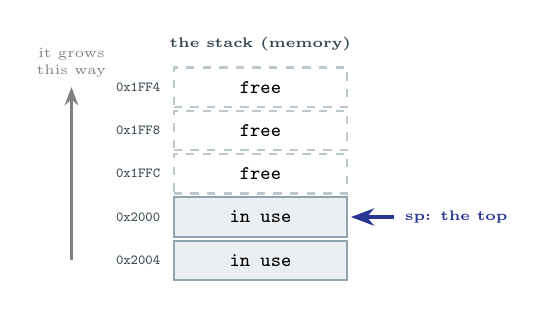
\begin{tikzpicture}[>=Stealth, font=\scriptsize,
      mcell/.style={draw=nLine, thick, fill=white, minimum width=2.2cm, minimum height=0.5cm, font=\ttfamily\scriptsize}]
    \node[font=\tiny\bfseries, text=nText] at (1.1,3.15) {the stack (memory)};
    \foreach \ad/\y in {0x1FF4/2.6, 0x1FF8/2.05, 0x1FFC/1.5, 0x2000/0.95, 0x2004/0.4}
      \node[addr, font=\ttfamily\tiny, anchor=east] at (-0.05,\y) {\ad};
    \foreach \y in {2.6, 2.05, 1.5} \node[mcell, dashed, draw=nLine!60] at (1.1,\y) {free};
    \foreach \y in {0.95, 0.4} \node[mcell, fill=nUsed] at (1.1,\y) {in use};
    \draw[<-, very thick, DeepBlue] (2.25,0.95) -- (2.8,0.95) node[right, font=\tiny\bfseries] {sp: the top};
    \draw[->, thick, gray] (-1.3,0.4) -- (-1.3,2.6) node[above, font=\tiny, align=center] {it grows\\this way};
  \end{tikzpicture}}

% ---------- one interrupt inside the CPU, from the signal to mret ----------
% #1 = step: 1 signal, 2 finish addi, 3 mepc, 4 jump, 5-7 prologue, 8-11 body, 12-14 epilogue, 15 mret
\newcommand{\irqpass}[1]{%
  \begin{tikzpicture}[>=Stealth, font=\scriptsize,
      mainstr/.style={instr, draw=nLine, fill=white},
      gi/.style={instr, draw=nLine, fill=white},
      runm/.style={instr, fill=white, aexec, label={[text=aExec, inner sep=1pt, font=\tiny]left:$\blacktriangleright$}},
      runi/.style={isrinstr, fill=white, aexec, label={[text=aExec, inner sep=1pt, font=\tiny]left:$\blacktriangleright$}},
      preg/.style={draw=nLine, very thick, fill=white, rounded corners=2pt, minimum width=2.0cm,
        minimum height=0.4cm, font=\ttfamily\scriptsize},
      mcell/.style={draw=nLine, thick, fill=white, minimum width=1.9cm, minimum height=0.38cm, font=\ttfamily\scriptsize},
      free/.style={mcell, dashed, draw=nLine!60},
      wr/.style={awrite, rounded corners=2pt},
      rd/.style={aread, rounded corners=2pt},
      flow/.style={->, very thick, DeepBlue}]
    \ifnum#1<5 \useasboundingbox (-2.1,-0.95) rectangle (14.75,3.55);
    \else \useasboundingbox (1.35,-0.95) rectangle (14.75,3.55); \fi
    % which instruction runs
    \ifnum#1<3 \def\runm{1}\else \def\runm{99}\fi
    \ifnum#1<5 \def\runi{99}\else\ifnum#1>15 \def\runi{99}\else \pgfmathtruncatemacro{\runi}{#1-5}\fi\fi
    % the main program: in full until the jump, then folded into one small box
    \ifnum#1<5
    \node[font=\scriptsize\bfseries, text=nText] at (1.3,3.35) {main program};
    \foreach \a/\t [count=\k from 0] in {0x0100/{li\ \ \ t0, 0}, 0x0104/{addi t0, t0, 1},
        0x0108/{sw\ \ \ t0, 0(a0)}, 0x010C/{j\ \ \ \ 0x0104}} {
      \ifnum\k=\runm \tikzset{cur/.style={runm}}\else \tikzset{cur/.style={mainstr}}\fi
      \node[addr, font=\ttfamily\tiny, anchor=east] at (0.15,{2.9-0.42*\k}) {\a};
      \node[cur, minimum width=2.2cm] (m\k) at (1.3,{2.9-0.42*\k}) {\t};
    }
    \else
    \node[draw=nLine, thick, fill=white, rounded corners=3pt, align=center, font=\tiny, inner sep=3pt] (mp) at (2.35,2.6)
      {\textcolor{nText}{\textbf{main program}}\\ \ifnum#1<15 paused\else continues\fi\\ at \texttt{0x0108}};
    \fi
    % the ISR in three parts
    \node[font=\scriptsize\bfseries, text=nText] at (4.9,3.35) {ISR: \texttt{onButtonA}};
    \foreach \a/\t [count=\k from 0] in {0x0200/{addi sp, sp, -16}, 0x0204/{sw\ \ \ t0, 12(sp)}, 0x0208/{sw\ \ \ t1, 8(sp)},
        0x020C/{la\ \ \ t0, presses}, 0x0214/{lw\ \ \ t1, 0(t0)}, 0x0218/{addi t1, t1, 1}, 0x021C/{sw\ \ \ t1, 0(t0)},
        0x0220/{lw\ \ \ t1, 8(sp)}, 0x0224/{lw\ \ \ t0, 12(sp)}, 0x0228/{addi sp, sp, 16}, 0x022C/{mret}} {
      \ifnum\k=\runi \tikzset{cur/.style={runi}}\else \tikzset{cur/.style={gi}}\fi
      \node[cur, minimum width=2.3cm, minimum height=0.3cm] (i\k) at (4.9,{3.0-0.3*\k}) {\t};
      \node[addr, font=\ttfamily\tiny, anchor=west] at (6.1,{3.0-0.3*\k}) {\a};
    }
    \ifnum#1<5 \def\part{0}\else\ifnum#1<8 \def\part{1}\else\ifnum#1<12 \def\part{2}\else \def\part{3}\fi\fi\fi
    \foreach \f/\l/\n/\q in {0/2/prologue/1, 3/6/body/2, 7/10/epilogue/3} {
      \ifnum\q=\part \def\pc{nText}\def\pf{\bfseries}\else \def\pc{gray!60}\def\pf{}\fi
      \draw[\pc, thick] ([xshift=1.0cm]i\f.north east) -- ++(0.12,0) |- ([xshift=1.0cm]i\l.south east);
      \node[anchor=west, font=\scriptsize\pf, text=\pc] at ($([xshift=1.2cm]i\f.north east)!0.5!([xshift=1.2cm]i\l.south east)$) {\n};
    }
    % values after the step: PC, mepc, t0, t1, sp, stack at 8(sp) and 12(sp), presses
    \ifcase#1 \or \def\pcv{0x0104}\def\mev{-}\def\tz{0}\def\to{5}\def\spv{0x2000}\def\sa{}\def\sb{}\def\pr{2}%
      \or \def\pcv{0x0104}\def\mev{-}\def\tz{1}\def\to{5}\def\spv{0x2000}\def\sa{}\def\sb{}\def\pr{2}%
      \or \def\pcv{0x0104}\def\mev{0x0108}\def\tz{1}\def\to{5}\def\spv{0x2000}\def\sa{}\def\sb{}\def\pr{2}%
      \or \def\pcv{0x0200}\def\mev{0x0108}\def\tz{1}\def\to{5}\def\spv{0x2000}\def\sa{}\def\sb{}\def\pr{2}%
      \or \def\pcv{0x0200}\def\mev{0x0108}\def\tz{1}\def\to{5}\def\spv{0x1FF0}\def\sa{?}\def\sb{?}\def\pr{2}%
      \or \def\pcv{0x0204}\def\mev{0x0108}\def\tz{1}\def\to{5}\def\spv{0x1FF0}\def\sa{1}\def\sb{?}\def\pr{2}%
      \or \def\pcv{0x0208}\def\mev{0x0108}\def\tz{1}\def\to{5}\def\spv{0x1FF0}\def\sa{1}\def\sb{5}\def\pr{2}%
      \or \def\pcv{0x020C}\def\mev{0x0108}\def\tz{0x1004}\def\to{5}\def\spv{0x1FF0}\def\sa{1}\def\sb{5}\def\pr{2}%
      \or \def\pcv{0x0214}\def\mev{0x0108}\def\tz{0x1004}\def\to{2}\def\spv{0x1FF0}\def\sa{1}\def\sb{5}\def\pr{2}%
      \or \def\pcv{0x0218}\def\mev{0x0108}\def\tz{0x1004}\def\to{3}\def\spv{0x1FF0}\def\sa{1}\def\sb{5}\def\pr{2}%
      \or \def\pcv{0x021C}\def\mev{0x0108}\def\tz{0x1004}\def\to{3}\def\spv{0x1FF0}\def\sa{1}\def\sb{5}\def\pr{3}%
      \or \def\pcv{0x0220}\def\mev{0x0108}\def\tz{0x1004}\def\to{5}\def\spv{0x1FF0}\def\sa{1}\def\sb{5}\def\pr{3}%
      \or \def\pcv{0x0224}\def\mev{0x0108}\def\tz{1}\def\to{5}\def\spv{0x1FF0}\def\sa{1}\def\sb{5}\def\pr{3}%
      \or \def\pcv{0x0228}\def\mev{0x0108}\def\tz{1}\def\to{5}\def\spv{0x2000}\def\sa{1}\def\sb{5}\def\pr{3}%
      \or \def\pcv{0x0108}\def\mev{0x0108}\def\tz{1}\def\to{5}\def\spv{0x2000}\def\sa{1}\def\sb{5}\def\pr{3}\fi
    % the CPU registers
    \draw[nLine, thick, rounded corners=4pt, fill=gray!4] (8.75,0.3) rectangle (11.15,3.5);
    \node[anchor=north west, font=\tiny\bfseries, text=nText] at (8.8,3.47) {CPU registers};
    \node[preg] (pc) at (9.95,2.9) {\textbf{PC}\ \ \pcv};
    \node[preg] (me) at (9.95,2.42) {\textbf{mepc}\ \ \mev};
    \node[preg] (t0) at (9.95,1.79) {\textbf{t0}\ \ \tz};
    \node[preg] (t1) at (9.95,1.31) {\textbf{t1}\ \ \to};
    \node[preg] (sp) at (9.95,0.68) {\textbf{sp}\ \ \spv};
    % the memory
    \node[font=\tiny\bfseries, text=nText, anchor=west] at (11.65,3.35) {memory};
    \node[addr, font=\ttfamily\tiny, anchor=east] at (12.15,2.95) {0x1004};
    \node[mcell] (pres) at (13.15,2.95) {presses = \pr};
    \node[font=\tiny\bfseries, text=nText, anchor=west] at (11.65,2.5) {the stack};
    \ifnum#1<5 \tikzset{st/.style={free}}\else\ifnum#1<14 \tikzset{st/.style={mcell, fill=nUsed}}\else \tikzset{st/.style={free, text=gray}}\fi\fi
    % two free cells above the frame: the border between free and in use is where sp points
    \foreach \ad/\y in {0x1FE8/2.1, 0x1FEC/1.74, 0x1FF0/1.38, 0x1FF4/1.02, 0x1FF8/0.66, 0x1FFC/0.30, 0x2000/-0.06}
      \node[addr, font=\ttfamily\tiny, anchor=east] at (12.15,\y) {\ad};
    \tikzset{scell/.style={minimum height=0.34cm}}
    \node[free, scell] at (13.15,2.1) {};
    \node[free, scell] at (13.15,1.74) {};
    \ifnum#1<5 \def\sq{}\else \def\sq{?}\fi
    \node[st, scell] at (13.15,1.38) {\sq};
    \node[st, scell] at (13.15,1.02) {\sq};
    \ifnum#1<7 \node[st, scell] (sb) at (13.15,0.66) {\sb}; \else \node[st, scell] (sb) at (13.15,0.66) {\sb\ (t1)}; \fi
    \ifnum#1<6 \node[st, scell] (sa) at (13.15,0.30) {\sa}; \else \node[st, scell] (sa) at (13.15,0.30) {\sa\ (t0)}; \fi
    \node[mcell, scell, fill=nUsed] at (13.15,-0.06) {main's data};
    \ifnum#1>4 \ifnum#1<14
      \draw[nText, thick] (14.15,1.55) -- ++(0.12,0) |- (14.15,0.13);
      \node[anchor=west, font=\tiny, text=nText, align=left] at (14.3,0.84) {16\\bytes};
    \fi\fi
    % signal, jump, return
    \ifnum#1=1
      \node[font=\scriptsize\bfseries, text=cIO, align=center] (sig) at (-1.4,2.9) {\faDotCircle\\interrupt!};
      \draw[flow, cIO] (sig.south) |- ([xshift=-0.95cm]m1.west);
    \fi
    \ifnum#1=2 \node[font=\tiny\bfseries, text=nInk, anchor=west] at ([xshift=2pt]m1.east) {\faCheck\ finished}; \fi
    \ifnum#1=3 \node[font=\tiny\bfseries, text=nText, anchor=north] at ([yshift=-2pt]m3.south) {$\uparrow$ \texttt{sw}: the next instruction}; \fi
    \ifnum#1=4 \draw[flow] (m1.east) to[out=0, in=180] node[pos=0.35, above, font=\tiny\bfseries] {jump} (i0.west); \fi
    \ifnum#1=15 \draw[flow] (i10.west) to[out=180, in=-90] node[pos=0.55, left, font=\tiny\bfseries] {return} (mp.south); \fi
    % what is read and written
    \ifnum#1=3 \draw[wr] (me.south west) rectangle (me.north east); \fi
    \ifnum#1=4 \draw[wr] (pc.south west) rectangle (pc.north east); \fi
    \ifnum#1=5 \draw[wr] (sp.south west) rectangle (sp.north east); \fi
    \ifnum#1=6 \draw[rd] (t0.south west) rectangle (t0.north east); \draw[wr] (sa.south west) rectangle (sa.north east); \fi
    \ifnum#1=7 \draw[rd] (t1.south west) rectangle (t1.north east); \draw[wr] (sb.south west) rectangle (sb.north east); \fi
    \ifnum#1=8 \draw[wr] (t0.south west) rectangle (t0.north east); \fi
    \ifnum#1=9 \draw[rd] (pres.south west) rectangle (pres.north east); \draw[wr] (t1.south west) rectangle (t1.north east); \fi
    \ifnum#1=10 \draw[wr] (t1.south west) rectangle (t1.north east); \fi
    \ifnum#1=11 \draw[rd] (t1.south west) rectangle (t1.north east); \draw[wr] (pres.south west) rectangle (pres.north east); \fi
    \ifnum#1=12 \draw[rd] (sb.south west) rectangle (sb.north east); \draw[wr] (t1.south west) rectangle (t1.north east); \fi
    \ifnum#1=13 \draw[rd] (sa.south west) rectangle (sa.north east); \draw[wr] (t0.south west) rectangle (t0.north east); \fi
    \ifnum#1=14 \draw[wr] (sp.south west) rectangle (sp.north east); \fi
    \ifnum#1=15 \draw[rd] (me.south west) rectangle (me.north east); \draw[wr] (pc.south west) rectangle (pc.north east); \fi
    % legend
    \node[font=\tiny] at (6.3,-0.7) {\textcolor{aExec}{$\blacktriangleright$}\ the instruction that runs
      \quad\tikz[baseline=-0.6ex]\draw[awrite] (0,-0.07) rectangle (0.32,0.11);\ written\quad\tikz[baseline=-0.6ex]\draw[aread] (0,-0.07) rectangle (0.32,0.11);\ read};
  \end{tikzpicture}}

% ---------- a C function and its stack, step by step ----------
% #1 = 0 before, 1 make room, 2 store a, 3 compute with a, 4 free the room
\newcommand{\cstack}[1]{%
  \begin{tikzpicture}[>=Stealth, font=\scriptsize,
      ins/.style={instr, draw=nLine, fill=white, minimum width=2.4cm, anchor=west},
      run/.style={ins, fill=white, aexec, label={[text=aExec, inner sep=1pt, font=\tiny]left:$\blacktriangleright$}},
      mcell/.style={draw=nLine, thick, fill=white, minimum width=2.0cm, minimum height=0.45cm, font=\ttfamily\scriptsize},
      preg/.style={draw=nLine, very thick, fill=white, rounded corners=2pt, minimum width=1.9cm,
        minimum height=0.45cm, font=\ttfamily\scriptsize},
      wr/.style={awrite, rounded corners=2pt},
      rd/.style={aread, rounded corners=2pt}]
    \useasboundingbox (-0.2,-0.9) rectangle (10.6,3.4);
    \ifcase#1 \def\ra{0}\def\rb{0}\or\def\ra{1}\def\rb{1}\or\def\ra{2}\def\rb{3}\or\def\ra{4}\def\rb{6}\or\def\ra{7}\def\rb{8}\fi
    \foreach \t/\c [count=\k from 1] in {{addi sp, sp, -16}/{make room}, {li\ \ \ a5, 7}/{}, {sw\ \ \ a5, 12(sp)}/{a = 7},
        {lw\ \ \ a5, 12(sp)}/{}, {addi a5, a5, 1}/{}, {mv\ \ \ a0, a5}/{return value}, {addi sp, sp, 16}/{free the room},
        {jr\ \ \ ra}/{return}} {
      \ifnum\k<\ra \tikzset{cur/.style={ins}}\else\ifnum\k>\rb \tikzset{cur/.style={ins}}\else \tikzset{cur/.style={run}}\fi\fi
      \node[cur] (k\k) at (0,{3.0-0.42*(\k-1)}) {\t};
      \node[font=\tiny, text=gray, anchor=west] at (2.5,{3.0-0.42*(\k-1)}) {\c};
    }
    \ifcase#1 \def\spv{0x2000}\def\topy{0.9}\def\av{}\def\afive{?}%
      \or\def\spv{0x1FF0}\def\topy{2.55}\def\av{}\def\afive{?}%
      \or\def\spv{0x1FF0}\def\topy{2.55}\def\av{7}\def\afive{7}%
      \or\def\spv{0x1FF0}\def\topy{2.55}\def\av{7}\def\afive{8}%
      \or\def\spv{0x2000}\def\topy{0.9}\def\av{7}\def\afive{8}\fi
    \draw[nLine, thick, rounded corners=4pt, fill=gray!4] (3.6,1.45) rectangle (5.85,3.25);
    \node[anchor=north west, font=\tiny\bfseries, text=nText] at (3.65,3.22) {CPU registers};
    \node[preg] (sp) at (4.72,2.45) {\textbf{sp}\ \ \spv};
    \node[preg] (a5) at (4.72,1.85) {\textbf{a5}\ \ \afive};
    \node[font=\tiny\bfseries, text=nText] at (8.6,3.2) {the stack};
    \foreach \ad/\y in {0x1FF0/2.55, 0x1FF4/2.1, 0x1FF8/1.65, 0x1FFC/1.2, 0x2000/0.75}
      \node[addr, font=\ttfamily\tiny, anchor=east] at (7.5,\y) {\ad};
    \ifnum#1=0 \tikzset{fr/.style={mcell, dashed, draw=nLine!60}}\else\ifnum#1=4 \tikzset{fr/.style={mcell, dashed, draw=nLine!60}}\else \tikzset{fr/.style={mcell, fill=nUsed}}\fi\fi
    \node[fr] at (8.6,2.55) {}; \node[fr] at (8.6,2.1) {}; \node[fr] at (8.6,1.65) {};
    \ifnum#1>1 \ifnum#1<4 \node[mcell, fill=nUsed] (va) at (8.6,1.2) {a = \av};
      \else \node[mcell, dashed, draw=nLine!60, text=gray] (va) at (8.6,1.2) {7 (free)}; \fi
    \else \node[fr] (va) at (8.6,1.2) {}; \fi
    \node[mcell, fill=nUsed] at (8.6,0.75) {in use};
    \ifnum#1=0 \def\topy{0.75}\else\ifnum#1=4 \def\topy{0.75}\else \def\topy{2.55}\fi\fi
    \draw[<-, very thick, DeepBlue] (9.65,\topy) -- (10.15,\topy) node[right, font=\tiny\bfseries] {sp};
    \ifnum#1>0 \ifnum#1<4
      \draw[nText, thick, decorate, decoration={brace, amplitude=4pt, mirror}] (6.8,2.8) -- (6.8,0.98)
        node[midway, left=4pt, font=\tiny, text=nText] {16 bytes};
    \fi\fi
    \ifnum#1=1 \draw[wr] (sp.south west) rectangle (sp.north east); \fi
    \ifnum#1=2 \draw[wr] (a5.south west) rectangle (a5.north east); \draw[wr] (va.south west) rectangle (va.north east); \fi
    \ifnum#1=3 \draw[rd] (va.south west) rectangle (va.north east); \draw[wr] (a5.south west) rectangle (a5.north east); \fi
    \ifnum#1=4 \draw[wr] (sp.south west) rectangle (sp.north east); \fi
    \node[font=\tiny] at (5.3,-0.6) {\textcolor{aExec}{$\blacktriangleright$}\ the instructions that run
      \quad\tikz[baseline=-0.6ex]\draw[awrite] (0,-0.07) rectangle (0.32,0.11);\ written\quad\tikz[baseline=-0.6ex]\draw[aread] (0,-0.07) rectangle (0.32,0.11);\ read};
  \end{tikzpicture}}

% ---------- the button with an interrupt (figure 1 of the course plan) ----------
\newcommand{\figbuttonisr}{%
  \begin{tikzpicture}[>=Stealth, font=\scriptsize]
    \draw[nInk, very thick, rounded corners=6pt, fill=nFill] (0,-0.3) rectangle (4.8,2.75);
    \node[anchor=north west, font=\scriptsize\bfseries, text=nInk] at (0.1,2.7) {\faMicrochip\ ESP32-C3};
    \node[lbox, draw=cISR, fill=cISR!15, minimum width=4.1cm, minimum height=0.85cm] (isr) at (2.4,1.6)
      {interrupt handler (ISR)\\[-1pt]{\ttfamily\mdseries presses++}};
    \node[lbox, draw=cWork, fill=cWork!12, minimum width=4.1cm, minimum height=0.85cm] (main) at (2.4,0.3)
      {main program\\[-1pt]{\mdseries does not check the button}};
    \draw[->, thick, dashed, DeepBlue] (isr.south) -- node[right, font=\tiny] {\texttt{presses}} (main.north);
    \node[lbox, draw=nInk, fill=nFill, minimum width=2.0cm] (btn) at (-2.3,1.6)
      {\faDotCircle\ Button A\\[-1pt]{\tiny\mdseries GPIO 5}};
    \draw[->, very thick, cISR] (btn.east) -- node[above, font=\tiny\bfseries] {interrupt} (isr.west);
    \node[draw=mygreen!60!black, fill=mygreen!55!black, rounded corners=2pt, minimum width=2.5cm,
      minimum height=0.8cm] (lcd) at (7.9,0.3) {};
    \node[fill=LcdScreen!45, minimum width=2.2cm, minimum height=0.5cm, font=\ttfamily\scriptsize] at (lcd) {Presses: 3};
    \node[font=\tiny, anchor=north] at (lcd.south) {LCD 16$\times$2};
    \draw[->, very thick, DeepBlue] (main.east) -- node[pos=0.62, above, font=\tiny] {GPIO 8, 9 (I2C)} (lcd.west);
  \end{tikzpicture}}

% ---------- a timer interrupt every 500 ms ----------
\newcommand{\timertimeline}{%
  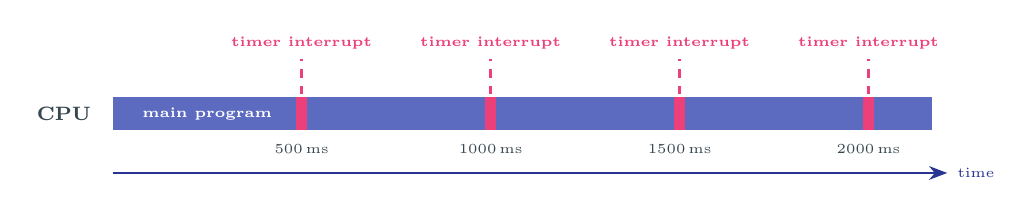
\begin{tikzpicture}[>=Stealth, font=\scriptsize]
    \node[anchor=east, font=\scriptsize\bfseries, text=nInk] at (-0.15,0) {CPU};
    \fill[cWork] (0,-0.21) rectangle (10.4,0.21);
    \node[font=\tiny\bfseries, text=white] at (1.2,0) {main program};
    \foreach \k in {1,...,4} {
      \fill[cISR] ({2.4*\k-0.07},-0.21) rectangle ({2.4*\k+0.07},0.21);
      \draw[cISR, thick, dashed] ({2.4*\k},0.25) -- ({2.4*\k},0.7);
      \node[font=\tiny\bfseries, text=cISR] at ({2.4*\k},0.9) {timer interrupt};
      \node[font=\tiny, text=nInk] at ({2.4*\k},-0.45) {\the\numexpr 500*\k\relax\,ms};
    }
    \draw[->, thick, DeepBlue] (0,-0.75) -- (10.6,-0.75) node[right, font=\tiny] {time};
  \end{tikzpicture}}

% ---------- a compiled C ISR overwrites a register of the main program ----------
\newcommand{\ctrouble}{%
  \begin{tikzpicture}[>=Stealth, font=\scriptsize,
      prog/.style={draw=nLine, fill=white, very thick, rounded corners=4pt, minimum width=3.0cm, minimum height=1.9cm},
      rv/.style={draw=nLine, very thick, fill=white, rounded corners=2pt, font=\ttfamily\scriptsize, inner sep=3pt}]
    \node[prog] (m1) at (0,0) {};
    \node[font=\scriptsize\bfseries, text=nText, anchor=north] at (m1.north) {main program};
    \node[font=\ttfamily\tiny, align=left] at (0,0.05) {li\ \ \ a5, 42\\\textcolor{gray}{\ldots}};
    \node[rv] at (0,-0.6) {a5 = 42};
    \node[prog] (isr) at (4.4,0) {};
    \node[font=\scriptsize\bfseries, text=nText, anchor=north] at (isr.north) {\texttt{onButtonA}, compiled};
    \node[font=\ttfamily\tiny, align=left] at (4.4,0.05) {lw\ \ \ a5, 4(a4)\\addi a5, a5, 1};
    \node[rv, awrite] at (4.4,-0.6) {a5 = 3};
    \node[prog] (m2) at (8.8,0) {};
    \node[font=\scriptsize\bfseries, text=nText, anchor=north] at (m2.north) {main program again};
    \node[font=\ttfamily\tiny, align=left] at (8.8,0.05) {add\ \ a0, a0, a5\\\textcolor{gray}{\ldots}};
    \node[rv, aread] at (8.8,-0.6) {a5 = 3 \textcolor{WriteRed}{\faTimes}};
    \draw[->, very thick, DeepBlue] (m1) -- node[above, font=\tiny\bfseries] {interrupt} (isr);
    \draw[->, very thick, DeepBlue] (isr) -- node[above, font=\tiny\bfseries] {return} (m2);
    \node[font=\tiny\bfseries, text=nText, anchor=north] at (8.8,-1.1) {it expected 42};
    \node[font=\tiny] at (4.4,-1.55) {\tikz[baseline=-0.6ex]\draw[awrite] (0,-0.07) rectangle (0.32,0.11);\ written\quad\tikz[baseline=-0.6ex]\draw[aread] (0,-0.07) rectangle (0.32,0.11);\ read};
  \end{tikzpicture}}

% ---------- a timer is a stopwatch with an alarm ----------
\newcommand{\timerblock}{%
  \begin{tikzpicture}[>=Stealth, font=\scriptsize,
      blk/.style={draw=nInk, very thick, rounded corners=4pt, fill=white, align=center, minimum height=1.45cm,
        inner sep=4pt}]
    \node[blk, minimum width=2.3cm] (clk) at (0,0) {\textbf{clock}\\[2pt]{\normalsize 1\,MHz}\\[1pt]{\tiny a pulse every 1\,$\mu$s}};
    \node[blk, minimum width=2.7cm] (cnt) at (3.5,0) {\textbf{counter}\\[2pt]{\ttfamily\normalsize 499\,998}\\[1pt]{\tiny +1 at every pulse}};
    \node[blk, draw=cISR, minimum width=2.7cm] (cmp) at (7.1,0) {\textbf{alarm?}\\[2pt]counter =\\{\ttfamily 500\,000}};
    \node[blk, fill=nFill, minimum width=2.0cm] (cpu) at (10.6,0) {\faMicrochip\ \textbf{CPU}\\[2pt]runs\\\texttt{onTimer}};
    \node[font=\Large, text=nInk] at (3.5,1.15) {\faStopwatch};
    \node[font=\Large, text=cISR] at (7.1,1.15) {\faBell};
    \draw[->, very thick, DeepBlue] (clk) -- node[above, font=\tiny] {pulses} (cnt);
    \draw[->, very thick, DeepBlue] (cnt) -- node[above, font=\tiny] {value} (cmp);
    \draw[->, very thick, cISR] (cmp) -- node[above, font=\tiny\bfseries] {interrupt!} (cpu);
    \draw[->, thick, cISR] (cmp.south) -- ++(0,-0.45) -| node[pos=0.25, below, font=\tiny] {and the counter starts again from 0} (cnt.south);
  \end{tikzpicture}}

% ---------- the counter of the timer over time ----------
\newcommand{\timersaw}{%
  \begin{tikzpicture}[>=Stealth, font=\scriptsize]
    \node[anchor=east, font=\scriptsize\bfseries, text=nInk, align=right] at (-0.15,0.75) {counter};
    \draw[gray, dashed] (0,1.5) -- (9.9,1.5) node[right, font=\tiny, text=cISR] {alarm: 500\,000};
    \node[anchor=east, font=\tiny, text=gray] at (-0.1,0) {0};
    \foreach \k in {0,...,3} {
      \draw[nInk, very thick] ({2.4*\k},0) -- ({2.4*(\k+1)},1.5);
      \draw[nInk, thick, dotted] ({2.4*(\k+1)},1.5) -- ({2.4*(\k+1)},0);
      \fill[cISR] ({2.4*(\k+1)},1.5) circle (0.09);
      \draw[->, cISR, thick] ({2.4*(\k+1)},-0.05) -- ({2.4*(\k+1)},-0.75);
    }
    \node[anchor=east, font=\scriptsize\bfseries, text=nInk] at (-0.15,-1.0) {CPU};
    \fill[cWork] (0,-1.21) rectangle (10.0,-0.79);
    \node[font=\tiny\bfseries, text=white] at (1.2,-1.0) {main program};
    \foreach \k in {1,...,4} {
      \fill[cISR] ({2.4*\k-0.08},-1.21) rectangle ({2.4*\k+0.08},-0.79);
      \node[font=\tiny, text=nInk] at ({2.4*\k},-1.42) {\the\numexpr 500*\k\relax\,ms};
    }
    \draw[->, thick, DeepBlue] (0,-1.7) -- (10.2,-1.7) node[right, font=\tiny] {time};
    \node[anchor=west, font=\tiny] at (0,-2.05) {\textcolor{cISR}{\faCircle}\ the counter reaches the alarm: an interrupt, and the ISR runs
      \quad\textcolor{cWork}{\rule{0.25cm}{0.2cm}}\ the main program};
  \end{tikzpicture}}

% ---------- where a timer can be ----------
\newcommand{\timerwhere}{%
  \begin{tikzpicture}[>=Stealth, font=\scriptsize,
      dev/.style={draw=nInk, thick, fill=white, rounded corners=2pt, minimum width=2.4cm, minimum height=0.55cm,
        font=\scriptsize, align=center}]
    % the board, as in Wokwi
    \pic (esp) at (0,0) {esp32c3};
    \node[font=\scriptsize\bfseries, text=nInk, anchor=south] at (1.35,5.45) {the board (as in Wokwi)};
    % the silver cover: the chip is under it
    \draw[nInk, very thick, dashed, rounded corners=1pt] (0.56,2.9) rectangle (2.14,5.36);
    % zoom
    \draw[nInk!60, thick] (2.14,5.36) -- (4.2,5.4);
    \draw[nInk!60, thick] (2.14,2.9) -- (4.2,0.3);
    % inside the chip
    \draw[nInk, very thick, rounded corners=5pt, fill=nFill] (4.2,0.3) rectangle (11.6,5.4);
    \node[anchor=north west, font=\scriptsize\bfseries, text=nInk] at (4.3,5.35) {inside the ESP32-C3 chip (under the silver cover)};
    \node[draw=nInk, very thick, fill=white, rounded corners=3pt, minimum width=1.3cm, minimum height=3.6cm,
      font=\scriptsize\bfseries, text=nInk, align=center] (core) at (5.1,2.55) {CPU\\core};
    % the interrupt controller with its table
    \node[draw=nInk, very thick, fill=white, rounded corners=3pt, inner sep=4pt, align=center] (ic) at (7.85,2.65)
      {\textbf{interrupt controller}\\[3pt]
       {\footnotesize\renewcommand{\arraystretch}{1.15}\begin{tabular}{|l|l|}\hline
         \badge{1}\ timer 0 & \texttt{onTimer} \\\hline
         \badge{2}\ GPIO 10 & \texttt{onAlarm} \\\hline
       \end{tabular}}};
    % the devices
    \node[dev] (tm) at (7.85,4.45) {timer 0\ \ \faStopwatch\quad timer 1\ \ \faStopwatch};
    \node[dev] (gp) at (7.85,0.85) {GPIO controller};
    \draw[->, very thick, nInk] (tm.south) -- (ic.north);
    \draw[->, very thick, nInk] (gp.north) -- (ic.south);
    \draw[->, very thick, nInk] (ic.west) -- (core.east |- ic.west);
    \node[font=\tiny, text=nInk, anchor=west] at (tm.east) {for us: \texttt{timerBegin}};
    \draw[<-, thick, nInk] (gp.east) -- ++(0.6,0) node[right, font=\tiny] {from the pins};
    % another chip, on a wire to GPIO 10 of the board
    \node[draw=nLine, very thick, fill=nFill, rounded corners=4pt, minimum width=1.7cm, minimum height=1.1cm,
      align=center, font=\scriptsize\bfseries, text=nInk] (rtc) at (-3.0,1.5) {another chip\\[-1pt]\faStopwatch};
    \node[font=\tiny, text=nInk, anchor=north] at (rtc.south) {e.g.\ a real-time clock};
    \node at (-3.0,2.35) {\badge{2}};
    \draw[very thick, WireGreen] (rtc.east) -- (esp-L10);
    \node[font=\tiny, text=nInk, anchor=south] at (-1.05,1.52) {a wire to GPIO 10};
  \end{tikzpicture}}

% ---------- one tick, three LEDs: #1 = number of ticks ----------
\newcommand{\tickleds}[1]{%
  \begin{tikzpicture}[font=\scriptsize]
    \pgfmathtruncatemacro{\tklast}{#1-1}
    \node[anchor=east, font=\scriptsize\bfseries, text=cISR] at (-0.15,0.55) {tick};
    \foreach \k in {1,...,#1} {
      \draw[cISR, very thick] ({0.42*\k},0.35) -- ({0.42*\k},0.75);
      \node[font=\tiny, text=nInk] at ({0.42*\k},0.95) {\k};
    }
    \foreach \p/\r/\n in {3/1/LED 1, 5/2/LED 2, 7/3/LED 3} {
      \pgfmathsetmacro{\yy}{-0.6*\r+0.3}
      \node[anchor=east, font=\scriptsize\bfseries] at (-0.15,\yy+0.08) {\n};
      \node[anchor=east, font=\tiny, text=gray!40!black] at (-0.15,\yy-0.16) {every \p\ ticks};
      \foreach \k in {0,...,\tklast} {
        \pgfmathtruncatemacro{\s}{mod(floor(\k/\p),2)}
        \ifnum\s=1
          \fill[cLed!75] ({0.42*\k},\yy-0.17) rectangle ({0.42*(\k+1)},\yy+0.17);
        \else
          \fill[gray!12] ({0.42*\k},\yy-0.17) rectangle ({0.42*(\k+1)},\yy+0.17);
        \fi
      }
      \foreach \k in {1,...,#1} {
        \pgfmathtruncatemacro{\rr}{mod(\k,\p)}
        \ifnum\rr=0 \draw[cISR, very thick] ({0.42*\k},\yy-0.24) -- ({0.42*\k},\yy+0.24); \fi
      }
    }
    \draw[decorate, decoration={brace, amplitude=3pt, mirror}, thick, nInk] (0.42,-1.8) -- (0.84,-1.8)
      node[midway, below=3pt, font=\tiny] {100 ms};
    \node[anchor=west, font=\tiny] at (2.0,-1.95) {\textcolor{cLed!75}{\rule{0.25cm}{0.2cm}}\ LED on
      \quad\textcolor{gray!25}{\rule{0.25cm}{0.2cm}}\ LED off
      \quad\textcolor{cISR}{\rule{0.06cm}{0.25cm}}\ the ISR changes the LED};
  \end{tikzpicture}}

% ---------- build it: two more LEDs (GPIO 7 and GPIO 3) ----------
% the circuit of Lecture 5 is faded, the new parts are drawn normally
\newcommand{\buildpicleds}{%
  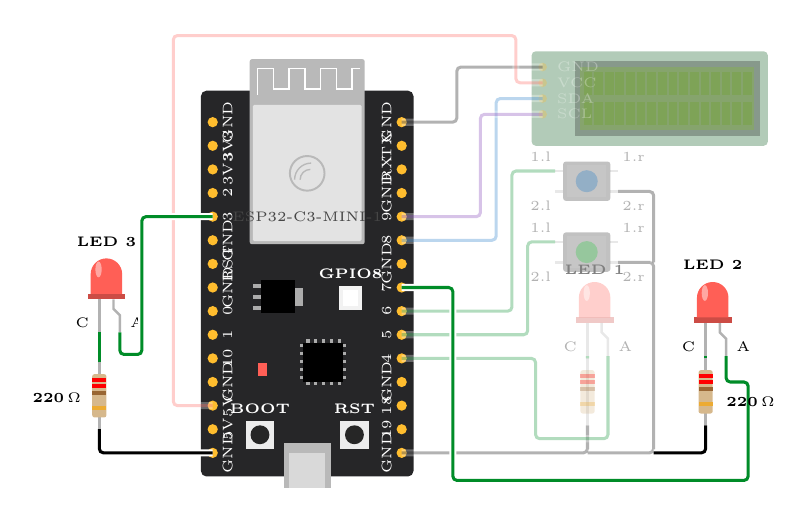
\begin{tikzpicture}[font=\tiny]
    \useasboundingbox (-2.2,-0.25) rectangle (7.3,5.7);
    \pic (esp) at (0,0) {esp32c3};
    \begin{scope}[opacity=0.3]
      % LED 1 and its resistor
      \pic (res) at (4.91,0.65) {wres};
      \pic (led) at (5.0,1.95) {wled};
      \draw[wire, black] (esp-R14) -- (4.91,0.3) -- (res-2);
      \draw[wire, WireGreen] (res-1) -- (led-C);
      \draw[wire, WireGreen] (esp-R10) -| (4.25,0.48) -| (led-A);
      % button A
      \pic (ba) at (4.9,2.85) {wbutton=MacGreen};
      \draw[wire, black] (ba-2r) -| (5.75,0.3) -- (4.91,0.3);
      \draw[wire, WireGreen] (esp-R9) -| ([xshift=-0.35cm]ba-1l) -- (ba-1l);
      % LCD
      \pic (lcd) at (4.2,4.2) {wlcd};
      \draw[wire, black] (esp-R0) -| ([xshift=-1.09cm]lcd-GND) -- (lcd-GND);
      \draw[wire, StorageBlue] (esp-R5) -| ([xshift=-0.59cm]lcd-SDA) -- (lcd-SDA);
      \draw[wire, ProgramPurple] (esp-R4) -| ([xshift=-0.79cm]lcd-SCL) -- (lcd-SCL);
      \draw[wire, MacRed] (esp-L12) -- (-0.35,0.9) -- (-0.35,5.6) -- (4.0,5.6) |- (lcd-VCC);
      % button B
      \pic (bb) at (4.9,3.75) {wbutton=StorageBlue};
      \draw[wire, black] (bb-2r) -| (5.75,2.72);
      \draw[wire, WireGreen] (esp-R8) -| ([xshift=-0.55cm]bb-1l) -- (bb-1l);
    \end{scope}
    \node[font=\fontsize{5.5}{6}\selectfont\bfseries, text=gray] at (5.0,2.62) {LED 1};
    % LED 2 on GPIO 7
    \pic (res2) at (6.41,0.65) {wres};
    \pic (led2) at (6.5,1.95) {wled};
    \draw[wire, black] (res2-2) -- (6.41,0.3) -- (5.75,0.3);
    \draw[wire, WireGreen] (res2-1) -- (led2-C);
    \draw[wire, WireGreen] (esp-R7) -- (3.2,2.4) -- (3.2,-0.05) -- (6.95,-0.05) -- (6.95,1.2) -- (6.67,1.2) -- (led2-A);
    \node[font=\fontsize{5.5}{6}\selectfont\bfseries, anchor=south] at (6.5,2.5) {LED 2};
    % LED 3 on GPIO 3
    \pic (res3) at (-1.29,0.6) {wres};
    \pic (led3) at (-1.2,2.25) {wled};
    \draw[wire, black] (res3-2) -- (-1.29,0.3) -- (esp-L14);
    \draw[wire, WireGreen] (res3-1) -- (led3-C);
    \draw[wire, WireGreen] (esp-L4) -- (-0.75,3.3) -- (-0.75,1.55) -- (-1.03,1.55) -- (led3-A);
    \node[font=\fontsize{5.5}{6}\selectfont\bfseries, anchor=south] at (-1.2,2.8) {LED 3};
    \node[font=\fontsize{5.5}{6}\selectfont\bfseries, anchor=east] at (-1.4,1.0) {220\,$\Omega$};
    \node[font=\fontsize{5.5}{6}\selectfont\bfseries, anchor=west] at (6.55,0.95) {220\,$\Omega$};
  \end{tikzpicture}}

% ---------- three LEDs, a button and the LCD (figure 2 of the course plan) ----------
\newcommand{\figthreeleds}{%
  \begin{tikzpicture}[>=Stealth, font=\scriptsize]
    \draw[nInk, very thick, rounded corners=6pt, fill=nFill] (0,-0.35) rectangle (4.0,3.75);
    \node[anchor=north west, font=\scriptsize\bfseries, text=nInk] at (0.1,3.7) {\faMicrochip\ ESP32-C3};
    \node[lbox, draw=cISR, fill=cISR!15, minimum width=3.5cm, minimum height=0.8cm] (tisr) at (2.0,2.6)
      {Timer ISR\\[-1pt]{\mdseries every 100 ms: 3 LEDs}};
    \node[lbox, draw=cISR, fill=cISR!15, minimum width=3.5cm, minimum height=0.8cm] (bisr) at (2.0,1.5)
      {Button ISR\\[-1pt]{\ttfamily\mdseries presses++}};
    \node[lbox, draw=cWork, fill=cWork!12, minimum width=3.5cm, minimum height=0.8cm] (main) at (2.0,0.4)
      {main loop\\[-1pt]{\mdseries counts}};
    \foreach \y/\g/\n in {3.3/4/1, 2.6/7/2, 1.9/3/3} {
      \draw[->, thick, cISR] (tisr.east) -- (5.35,\y);
      \fill[cLed] (5.55,\y) circle (0.15);
      \node[anchor=west, font=\scriptsize] at (5.8,\y) {LED \n\ (GPIO \g)};
    }
    \node[lbox, draw=nInk, fill=nFill, minimum width=1.9cm] (btn) at (-1.9,1.5)
      {\faDotCircle\ Button A\\[-1pt]{\mdseries GPIO 5}};
    \draw[->, very thick, cISR] (btn.east) -- (bisr.west);
    \node[draw=mygreen!60!black, fill=mygreen!55!black, rounded corners=2pt, minimum width=2.6cm,
      minimum height=1.05cm] (lcd) at (6.4,0.4) {};
    \node[fill=LcdScreen!45, minimum width=2.3cm, minimum height=0.8cm, font=\ttfamily\scriptsize, align=left] at (lcd)
      {Presses: 3\\Loop: 18452};
    \draw[->, very thick, DeepBlue] (main.east) -- (lcd.west);
  \end{tikzpicture}}

% ---------- inside the ESP32-C3: the interrupt controller finds and starts the ISR ----------
% #1 = step: 1 the pin changes, 2 the controller looks up the function, 3 the CPU runs the ISR
\newcommand{\figintctrl}[1]{%
  \ifnum#1=1 \tikzset{icst/.style={line width=2.4pt}}\else \tikzset{icst/.style={line width=1.2pt}}\fi
  \ifnum#1=2 \tikzset{tabst/.style={draw=cISR, line width=2pt}}\else \tikzset{tabst/.style={draw=DeepBlue!60, line width=0.6pt}}\fi
  \ifnum#1=3 \tikzset{isrst/.style={line width=2.4pt}}\else \tikzset{isrst/.style={line width=1.2pt, opacity=0.3}}\fi
  \ifnum#1>1 \def\isrlbl{ISR: }\else \def\isrlbl{}\fi
  \begin{tikzpicture}[>=Stealth, font=\scriptsize]
    \draw[nInk, very thick, rounded corners=6pt, fill=nFill] (0,-1.15) rectangle (9.2,3.0);
    \node[anchor=north west, font=\scriptsize\bfseries, text=nInk] at (0.1,2.95) {\faMicrochip\ ESP32-C3};
    \node[lbox, draw=nInk, fill=nFill, minimum width=1.9cm] (btn) at (-2.1,1.4)
      {\faDotCircle\ Button A\\[-1pt]{\tiny\mdseries GPIO 5}};
    \node[lbox, draw=cISR, fill=cISR!15, minimum width=2.4cm, minimum height=0.95cm, icst] (ic) at (1.75,1.4) {interrupt\\controller};
    \node[tabst, fill=white, rounded corners=2pt,
      align=left, font=\tiny\ttfamily, inner sep=4pt] (tab) at (1.75,-0.2)
      {GPIO 5 $\to$ onButtonA\\GPIO 6 $\to$ (none)};
    \node[font=\tiny, text=gray, anchor=north] at (tab.south) {filled by \texttt{attachInterrupt}};
    \node[draw=nInk, very thick, rounded corners=4pt, fill=white, minimum width=3.6cm, minimum height=2.9cm] (cpu) at (6.9,1.05) {};
    \node[font=\scriptsize\bfseries, text=nInk, anchor=north] at (6.9,2.45) {CPU};
    \node[lbox, draw=cWork, fill=cWork!12, minimum width=3.0cm] (main) at (6.9,1.55)
      {main program\ifnum#1>2\\[-1pt]{\tiny\mdseries suspended}\fi};
    \node[lbox, draw=cISR, fill=cISR!15, minimum width=3.0cm, isrst] (isr) at (6.9,0.3)
      {\isrlbl\texttt{onButtonA()}\\[-1pt]{\ttfamily\mdseries presses++}};
    \draw[->, very thick, cIO] (btn.east) -- node[above] {\badge{1}} (ic.west);
    \ifnum#1>1 \draw[<->, thick, cISR] (ic.south) -- node[right] {\badge{2}} (tab.north); \fi
    \ifnum#1>2 \draw[->, very thick, cISR] (ic.east) -- ++(0.55,0) |- node[pos=0.75, above] {\badge{3}} (isr.west); \fi
  \end{tikzpicture}}

% a highlighted piece of code inside a listing: (*\hlcode{...}*)
\newcommand{\hlcode}[1]{{\setlength{\fboxsep}{1pt}\colorbox{AccentOrange}{\textcolor{white}{\bfseries #1}}}}
% the end of the highlighted line, inside a listing: (*\eol*)
\newcommand{\eol}{\tikz[remember picture, overlay]\coordinate (eol) at (0,0.08);}
% one note with an arrow to the line that ends with \eol; #1 = vertical shift, #2 = title, #3 = text
\newcommand{\codenote}[3][0pt]{%
  \begin{tikzpicture}[remember picture, overlay, >=Stealth]
    \node[draw=AccentOrange, very thick, fill=AccentOrange!6, rounded corners=4pt, text width=0.33\paperwidth,
      align=left, inner sep=6pt, font=\footnotesize, anchor=west] (cal)
      at ([yshift=#1]eol -| {$(current page.west)!0.6!(current page.east)$}) {\textbf{\textcolor{AccentOrange}{#2}}\\[3pt]#3};
    \draw[->, very thick, AccentOrange] (eol -| cal.west) -- ([xshift=4pt]eol);
  \end{tikzpicture}}

% ---------- three ways to keep a rhythm: #1 = 1 delay(), 2 millis() in loop(), 3 timer interrupt ----------
\newcommand{\rhythm}[1]{%
  \begin{tikzpicture}[>=Stealth, font=\tiny]
    \useasboundingbox (-0.1,-1.0) rectangle (4.6,0.95);
    \ifnum#1=1
      \node[draw=white, fill=cIdle, minimum width=0.9cm, minimum height=0.42cm, inner sep=0pt, anchor=west,
        font=\tiny\bfseries, text=white] at (0,0) {LED 1};
      \node[draw=white, fill=cIdle, minimum width=1.5cm, minimum height=0.42cm, inner sep=0pt, anchor=west,
        font=\tiny\bfseries, text=white] at (0.9,0) {wait for LED 2};
      \node[draw=white, fill=cIdle, minimum width=2.1cm, minimum height=0.42cm, inner sep=0pt, anchor=west,
        font=\tiny\bfseries, text=white] at (2.4,0) {wait for LED 3};
      \node[font=\tiny\bfseries, text=nInk, anchor=south] at (2.25,0.3) {\texttt{delay}: 300 + 500 + 700 ms, one after another};
      \draw[<->, thick, AccentOrange] (0,-0.45) -- node[below, font=\tiny\bfseries] {LED 1 changes again only after 1.5 s} (4.5,-0.45);
    \else
      \fill[cWork] (0,-0.21) rectangle (4.5,0.21);
      \foreach \a in {0.5,1.6,2.6,3.5} {
        \fill[cIdle] (\a,-0.21) rectangle (\a+0.6,0.21);
        \node[font=\tiny\bfseries, text=white] at (\a+0.3,0) {LCD};
      }
      \foreach \x in {0.9,1.8,2.7,3.6} \draw[nInk, dashed, thick] (\x,0.25) -- (\x,0.6);
      \node[font=\tiny, text=nInk, anchor=south] at (2.25,0.6) {when LED 1 should change};
    \fi
    \ifnum#1=2
      \foreach \x/\y in {0.9/1.1, 1.8/2.2, 2.7/3.2, 3.6/4.1} {
        \draw[AccentOrange, very thick] (\y,-0.28) -- (\y,-0.55);
        \draw[->, nInk, thick] (\x,-0.42) -- (\y-0.03,-0.42);
      }
      \node[font=\tiny\bfseries, text=AccentOrange, anchor=north] at (2.25,-0.6) {LED 1 changes late: after each LCD write};
    \fi
    \ifnum#1=3
      \foreach \x in {0.9,1.8,2.7,3.6} {
        \fill[cISR] (\x-0.04,-0.21) rectangle (\x+0.04,0.21);
        \draw[cISR, very thick] (\x,-0.28) -- (\x,-0.55);
      }
      \node[font=\tiny\bfseries, text=cISR, anchor=north] at (2.25,-0.6) {LED 1 changes on time, even during the LCD write};
    \fi
  \end{tikzpicture}}

% ---------- one core, three tasks ----------
\newcommand{\oneprocessor}{%
  \begin{tikzpicture}[>=Stealth, font=\scriptsize]
    \foreach \n/\c/\w/\y in {A/cTaskA/drive the motors/1.3, B/cTaskB/look for obstacles/0, C/cTaskC/update the screen/-1.3} {
      \node[lbox, draw=\c, fill=\c!12, minimum width=3.6cm, minimum height=0.95cm, anchor=west] (t\n) at (0,\y)
        {Task \n: {\mdseries \w}\\[-1pt]{\ttfamily\mdseries for (;;) \{ \ldots\ \}}};
      \draw[->, very thick, DeepBlue] (t\n.east) -- (5.6,0) node[pos=0.45, fill=white, font=\small\bfseries,
        text=AccentOrange, inner sep=1pt] {?};
    }
    \node[cpubox, minimum width=2.6cm, minimum height=1.6cm] at (6.9,0)
      {CPU core\\[-1pt]{\tiny\mdseries one instruction at a time}};
  \end{tikzpicture}}

% ---------- time slices, and how it looks to us ----------
\newcommand{\timeslices}{%
  \begin{tikzpicture}[>=Stealth, font=\scriptsize]
    \tlbar{0}{CPU core}{0.7/cTaskA/A,0.7/cTaskB/B,0.7/cTaskC/C,0.7/cTaskA/A,0.7/cTaskB/B,0.7/cTaskC/C,
      0.7/cTaskA/A,0.7/cTaskB/B,0.7/cTaskC/C,0.7/cTaskA/A,0.7/cTaskB/B,0.7/cTaskC/C}
    \draw[decorate, decoration={brace, amplitude=3pt}, thick, nInk] (0,0.28) -- (0.7,0.28)
      node[midway, above=3pt, font=\tiny] {1 ms};
    \node[anchor=west, font=\scriptsize\bfseries, text=nInk] at (0,-0.65) {How it looks to us:};
    \tlbar{-1.15}{task A}{8.4/cTaskA/blinks the LEDs}
    \tlbar{-1.65}{task B}{8.4/cTaskB/counts on the LCD}
    \tlbar{-2.15}{task C}{8.4/cTaskC/reads the buttons}
    \draw[->, thick, DeepBlue] (0,-2.6) -- (8.6,-2.6) node[right, font=\tiny] {time};
  \end{tikzpicture}}

% ---------- the tick wakes the scheduler ----------
\newcommand{\tickscheduler}{%
  \begin{tikzpicture}[>=Stealth, font=\scriptsize]
    \node[lbox, draw=cISR, fill=cISR!15, minimum width=1.8cm, minimum height=0.9cm] (tim) at (0,0) {\faClock\ timer};
    \node[lbox, draw=cSched, fill=cSched!20, minimum width=2.3cm, minimum height=0.9cm] (sch) at (3.7,0)
      {scheduler\\[-1pt]{\tiny\mdseries which task next?}};
    \draw[->, very thick, cISR] (tim) -- node[above, font=\tiny\bfseries] {tick} node[below, font=\tiny] {every 1 ms} (sch);
    \node[lbox, draw=cTaskA, fill=cTaskA!12, minimum width=1.5cm] (a) at (7.0,1.0) {Task A};
    \node[lbox, draw=cTaskB, fill=cTaskB!25, minimum width=1.5cm, line width=2pt] (b) at (7.0,0) {Task B};
    \node[lbox, draw=cTaskC, fill=cTaskC!12, minimum width=1.5cm] (c) at (7.0,-1.0) {Task C};
    \draw[->, thick, DeepBlue!50] (sch.east) -- (a.west);
    \draw[->, line width=2pt, DeepBlue] (sch.east) -- (b.west);
    \draw[->, thick, DeepBlue!50] (sch.east) -- (c.west);
    \node[anchor=west, font=\tiny\bfseries, text=sAmberText] at (7.85,0) {runs now};
  \end{tikzpicture}}

% ---------- each task has its own stack ----------
\newcommand{\stackmem}{%
  \begin{tikzpicture}[>=Stealth, font=\scriptsize]
    \node[font=\scriptsize\bfseries, text=nInk] at (1.2,4.55) {Memory (RAM)};
    \draw[nLine, fill=gray!8] (0,0) rectangle (2.4,4.3);
    \node[font=\tiny, text=gray!40!black] at (1.2,4.05) {global variables};
    \foreach \n/\c/\yb/\h in {A/cTaskA/2.7/0.7, B/cTaskB/1.45/0.45, C/cTaskC/0.2/0.6} {
      \draw[\c, thick, fill=white] (0.2,\yb) rectangle (2.2,\yb+1.05);
      \fill[\c!30] (0.2,\yb) rectangle (2.2,\yb+\h);
      \node[font=\tiny\bfseries, text=\c] at (1.2,\yb+0.86) {stack of task \n};
    }
    \foreach \n/\c/\t in {B/cTaskB/1.9, C/cTaskC/0.8} {
      \draw[->, thick, \c] (2.85,\t) -- (2.25,\t);
      \node[anchor=west, font=\tiny, text=\c] at (2.85,\t) {top of \n};
    }
    \node[cpubox, minimum width=1.6cm, minimum height=1.1cm] (cpu) at (5.1,3.4) {};
    \node[font=\tiny\bfseries, text=white, anchor=north] at (cpu.north) {CPU};
    \node[reg, minimum width=1.2cm] (sp) at (5.1,3.25) {\textbf{sp}};
    \draw[->, very thick, AccentOrange] (sp.west) -- (2.25,3.4) node[pos=0.45, above, font=\tiny\bfseries] {top of A};
  \end{tikzpicture}}

% ---------- context switch in 4 steps ----------
% ---------- a context switch with the code: task A, the tick handler (simplified), task B ----------
% #1 step: 1 A runs, 2 tick: save A, 3 scheduler, 4 switch the stack, 5 restore B and B runs
\newcommand{\ctxpass}[1]{%
  \begin{tikzpicture}[>=Stealth, font=\scriptsize,
      ln/.style={draw=nLine, fill=white, minimum height=0.38cm, inner sep=1pt, font=\ttfamily\scriptsize,
        anchor=west, text width=2.95cm},
      lnh/.style={ln, text width=4.6cm},
      run/.style={aexec, label={[text=aExec, inner sep=1pt, font=\tiny]left:$\blacktriangleright$}},
      preg/.style={draw=nLine, very thick, fill=white, rounded corners=2pt, minimum width=2.5cm,
        minimum height=0.42cm, font=\scriptsize},
      mcell/.style={draw=nLine, thick, fill=nUsed, minimum width=2.6cm, minimum height=0.42cm, inner sep=0pt,
        font=\tiny},
      free/.style={mcell, fill=white, dashed, draw=nLine!60}]
    \useasboundingbox (-0.3,-0.7) rectangle (14.6,5.85);
    % which line runs
    \ifnum#1=1 \def\ra{1}\else \def\ra{99}\fi
    \ifnum#1=5 \def\rb{2}\else \def\rb{99}\fi
    \ifcase#1 \or \def\rh{99}\or \def\rh{0}\or \def\rh{1}\or \def\rh{2}\or \def\rh{99}\fi
    % ----- task A -----
    \node[font=\scriptsize\bfseries, text=nText, anchor=west] at (0.4,5.6) {task A \mdseries(blinks the LED)};
    \foreach \a/\t [count=\k from 0] in {0x0208/{li\ \ \ t0, 0}, 0x020C/{addi t0, t0, 1}, 0x0210/{sw\ \ \ t0, 0(a0)},
        0x0214/{j\ \ \ \ 0x020C}} {
      \ifnum\k=\ra \tikzset{cur/.style={ln, run}}\else \tikzset{cur/.style={ln}}\fi
      \node[cur] at (0.4,{5.15-0.42*\k}) {\a\ \ \t};
    }
    \ifnum#1>1 \node[font=\tiny, text=gray, anchor=west] at (0.4,3.5) {paused, next: \texttt{0x0210}}; \fi
    % ----- the tick handler -----
    \node[font=\scriptsize\bfseries, text=nText, anchor=west] at (4.75,5.6) {tick handler \mdseries(simplified)};
    \foreach \t [count=\k from 0] in {{save all registers + PC on its stack}, {next = scheduler()},
        {sp = the stack of next}, {restore all registers + PC, return}} {
      \ifnum\k=\rh \tikzset{cur/.style={lnh, run}}\else \tikzset{cur/.style={lnh}}\fi
      \node[cur] at (4.75,{5.15-0.42*\k}) {\t};
    }
    % ----- task B -----
    \node[font=\scriptsize\bfseries, text=nText, anchor=west] at (10.95,5.6) {task B \mdseries(counts)};
    \foreach \a/\t [count=\k from 0] in {0x0300/{li\ \ \ t0, 0}, 0x0304/{add\ \ t0, t0, t1}, 0x0308/{addi t1, t1, 1},
        0x030C/{j\ \ \ \ 0x0304}} {
      \ifnum\k=\rb \tikzset{cur/.style={ln, run}}\else \tikzset{cur/.style={ln}}\fi
      \node[cur] at (10.95,{5.15-0.42*\k}) {\a\ \ \t};
    }
    \ifnum#1<5 \node[font=\tiny, text=gray, anchor=west] at (10.95,3.5) {paused, next: \texttt{0x0308}}; \fi
    % ----- the stacks, under their tasks; two free cells above the used part -----
    \node[font=\tiny\bfseries, text=nText] at (1.9,2.65) {stack of A};
    \node[font=\tiny\bfseries, text=nText] at (12.45,2.65) {stack of B};
    \foreach \x/\n in {1.9/A, 12.45/B} {
      \node[mcell] at (\x,0.2) {data of \n};
      \node[mcell] (d\n) at (\x,0.62) {data of \n};
    }
    \ifnum#1<2
      \node[free] (cA) at (1.9,1.04) {};
    \else
      \node[mcell] (cA) at (1.9,1.04) {A's PC (0x0210) + registers};
    \fi
    \node[free] at (1.9,1.46) {}; \node[free] at (1.9,1.88) {};
    \ifnum#1<5
      \node[mcell] (cB) at (12.45,1.04) {B's PC (0x0308) + registers};
    \else
      \node[free, text=gray] (cB) at (12.45,1.04) {B's PC (0x0308) + registers};
    \fi
    \node[free] at (12.45,1.46) {}; \node[free] at (12.45,1.88) {};
    % ----- the CPU, in the middle -----
    \ifcase#1 \or \def\pcv{0x020C}\def\who{A's}\or \def\pcv{in the handler}\def\who{A's}\or \def\pcv{in the handler}\def\who{A's}%
      \or \def\pcv{in the handler}\def\who{A's}\or \def\pcv{0x0308}\def\who{B's}\fi
    \draw[nLine, thick, rounded corners=4pt, fill=gray!4] (5.9,0.25) rectangle (8.45,2.45);
    \node[anchor=north west, font=\tiny\bfseries, text=nText] at (5.95,2.42) {CPU};
    \node[preg] (pc) at (7.18,1.8) {\textbf{PC}\ \ \texttt{\pcv}};
    \node[preg] (rg) at (7.18,1.28) {\textbf{registers}\ \ \who};
    \node[preg] (sp) at (7.18,0.68) {\textbf{sp}};
    \ifnum#1=1 \draw[->, very thick, nInk] (sp.west) -- (dA.east); \fi
    \ifnum#1=2 \draw[->, very thick, nInk] (sp.west) -- (cA.east); \fi
    \ifnum#1=3 \draw[->, very thick, nInk] (sp.west) -- (cA.east); \fi
    \ifnum#1=4 \draw[->, very thick, nInk] (sp.east) -- (cB.west); \fi
    \ifnum#1=5 \draw[->, very thick, nInk] (sp.east) -- (dB.west); \fi
    % ----- what is read and written -----
    \ifnum#1=2 \draw[aread] (rg.south west) rectangle (pc.north east); \draw[awrite] (cA.south west) rectangle (cA.north east); \fi
    \ifnum#1=4 \draw[awrite] (sp.south west) rectangle (sp.north east); \fi
    \ifnum#1=5 \draw[aread] (cB.south west) rectangle (cB.north east); \draw[awrite] (rg.south west) rectangle (pc.north east); \fi
    \ifnum#1=2 \node[font=\scriptsize\bfseries, text=cIO, anchor=west] at (7.6,5.6) {\faClock\ tick!}; \fi
    % ----- legend -----
    \node[font=\tiny] at (7.18,-0.45) {\textcolor{aExec}{$\blacktriangleright$}\ the code that runs
      \quad\tikz[baseline=-0.6ex]\draw[awrite] (0,-0.07) rectangle (0.32,0.11);\ written
      \quad\tikz[baseline=-0.6ex]\draw[aread] (0,-0.07) rectangle (0.32,0.11);\ read};
  \end{tikzpicture}}

% #1 = step (1 tick, 2 save A, 3 choose B, 4 restore B)
\newcommand{\ctxswitch}[1]{%
  \begin{tikzpicture}[>=Stealth, font=\scriptsize,
      cell/.style={draw=nLine, minimum width=1.8cm, minimum height=0.42cm, inner sep=0pt, font=\ttfamily\tiny},
      src/.style={aread},
      dst/.style={awrite},
      tcell/.style={draw=nLine, fill=white, minimum height=0.45cm, inner sep=0pt}]
    \useasboundingbox (-0.2,-0.7) rectangle (12.5,4.75);
    % ----- the CPU -----
    \draw[nLine, very thick, rounded corners=6pt, fill=gray!4] (0,0) rectangle (3.0,3.6);
    \node[anchor=north west, font=\scriptsize\bfseries, text=nText] at (0.08,3.55) {CPU};
    \ifcase#1 \or \def\running{task A}\or \def\running{scheduler}\or \def\running{scheduler}\or \def\running{task B}\fi
    \node[anchor=north east, font=\tiny] at (2.95,3.55) {running: \textbf{\running}};
    \ifnum#1<4 \colorlet{ctxc}{cTaskA}\def\who{A}\else \colorlet{ctxc}{cTaskB}\def\who{B}\fi
    \foreach \r/\y in {PC/2.75, t0/2.1, t1/1.45} {
      \node[draw=nLine, very thick, fill=white, rounded corners=2pt, minimum width=2.4cm, minimum height=0.48cm,
        font=\ttfamily\scriptsize] at (1.5,\y) {\textbf{\r}\ \ \who's \r};
    }
    \node[draw=nLine, very thick, fill=white, rounded corners=2pt, minimum width=2.4cm, minimum height=0.48cm,
      font=\ttfamily\scriptsize] at (1.5,0.55) {\textbf{sp}\ \ top of \who};
    \ifnum#1=2
      \draw[src, rounded corners=3pt] (0.22,1.14) rectangle (2.78,3.06);
      \draw[src, rounded corners=3pt] (0.22,0.24) rectangle (2.78,0.86);
    \fi
    \ifnum#1=4
      \draw[dst, rounded corners=3pt] (0.22,1.14) rectangle (2.78,3.06);
      \draw[dst, rounded corners=3pt] (0.22,0.24) rectangle (2.78,0.86);
    \fi
    % ----- the two stacks -----
    \foreach \sx/\n/\c in {4.9/A/cTaskA, 7.6/B/cTaskB} {
      \node[font=\scriptsize\bfseries, text=nText] at (\sx,3.3) {stack of \n};
      \draw[nLine, thick] (\sx-0.95,0.15) rectangle (\sx+0.95,3.0);
      \node[cell, fill=nUsed, font=\tiny] at (\sx,0.45) {data of \n};
      \node[cell, fill=nUsed, font=\tiny] at (\sx,0.87) {data of \n};
    }
    \ifnum#1>1
      \foreach \r/\y in {t1/1.29, t0/1.71, PC/2.13} \node[cell, fill=nUsed] at (4.9,\y) {A's \r};
    \else
      \foreach \y in {1.29,1.71,2.13} \node[cell, draw=nLine!50, dashed] at (4.9,\y) {};
    \fi
    \ifnum#1=2 \draw[dst, rounded corners=2pt] (3.98,1.06) rectangle (5.82,2.36); \fi
    \foreach \r/\y in {t1/1.29, t0/1.71, PC/2.13} \node[cell, fill=nUsed] at (7.6,\y) {B's \r};
    \ifnum#1=4 \draw[src, rounded corners=2pt] (6.68,1.06) rectangle (8.52,2.36); \fi
    % top of each stack
    \ifnum#1>1 \def\topA{2.34}\else \def\topA{1.08}\fi
    \ifnum#1>3 \def\topB{1.08}\else \def\topB{2.34}\fi
    \draw[->, thick, nText] (6.15,\topA) -- (5.88,\topA);
    \node[anchor=west, font=\tiny, text=nText] at (6.12,\topA) {top};
    \draw[->, thick, nText] (8.85,\topB) -- (8.58,\topB);
    \node[anchor=west, font=\tiny, text=nText] at (8.82,\topB) {top};
    % ----- the table of saved stack pointers -----
    \node[draw=nLine, fill=gray!25, text=nText, font=\tiny\bfseries, minimum width=2.6cm, minimum height=0.42cm]
      at (10.7,3.0) {saved sp};
    \ifnum#1>1 \def\valA{top of A}\else \def\valA{-}\fi
    \node[tcell, minimum width=0.9cm, font=\tiny\bfseries, text=nText] at (9.85,2.55) {task A};
    \node[tcell, minimum width=1.7cm, font=\ttfamily\tiny] (va) at (11.15,2.55) {\valA};
    \node[tcell, minimum width=0.9cm, font=\tiny\bfseries, text=nText] at (9.85,2.1) {task B};
    \node[tcell, minimum width=1.7cm, font=\ttfamily\tiny] (vb) at (11.15,2.1) {top of B};
    \ifnum#1=2 \draw[dst] (va.south west) rectangle (va.north east); \fi
    \ifnum#1=3 \draw[nText, line width=1.6pt, dashed] (9.4,1.875) rectangle (12.0,2.325); \fi
    \ifnum#1=4 \draw[src] (vb.south west) rectangle (vb.north east); \fi
    % ----- legend -----
    \node[font=\tiny, anchor=west] at (4.1,4.4) {\tikz[baseline=-0.6ex]\draw[aread] (0,-0.07) rectangle (0.32,0.11);\ read from here
      \quad\tikz[baseline=-0.6ex]\draw[awrite] (0,-0.07) rectangle (0.32,0.11);\ written here};
    % ----- what happens in this step -----
    \ifnum#1=1
      \node[lbox, draw=cIO, fill=cIO!12, text=cIO!60!black] (tick) at (1.5,4.3) {\faClock\ tick: timer interrupt};
      \draw[->, very thick, cIO] (tick) -- (1.5,3.62);
    \fi
    \ifnum#1=2
      \draw[->, very thick, DeepBlue] (2.8,2.1) -- (3.96,1.71);
      \draw[->, very thick, DeepBlue, rounded corners=3pt] (2.8,0.55) -- (3.4,0.55) -- (3.4,-0.45) -- (12.3,-0.45)
        -- (12.3,2.55) -- (12.02,2.55);
    \fi
    \ifnum#1=3
      \node[lbox, draw=nLine, fill=white] (sch) at (10.7,1.1) {scheduler: next task = B};
      \draw[->, very thick, DeepBlue] (sch) -- (10.7,1.86);
    \fi
    \ifnum#1=4
      \draw[->, very thick, DeepBlue, rounded corners=3pt] (12.02,2.1) -- (12.3,2.1) -- (12.3,-0.45) -- (3.4,-0.45)
        -- (3.4,0.55) -- (2.82,0.55);
      \draw[->, very thick, DeepBlue, rounded corners=3pt] (8.54,1.71) -- (9.0,1.71) -- (9.0,3.75) -- (3.3,3.75)
        -- (3.3,2.1) -- (2.82,2.1);
    \fi
  \end{tikzpicture}}
\newcommand{\ctxlegend}{%
  {\tiny\tikz[baseline=-0.6ex]\draw[aread] (0,-0.07) rectangle (0.32,0.11);\ read from here
  \qquad\tikz[baseline=-0.6ex]\draw[awrite] (0,-0.07) rectangle (0.32,0.11);\ written here}}

% ---------- task states ----------
\newcommand{\taskstates}{%
  \begin{tikzpicture}[>=Stealth, font=\scriptsize,
      st/.style={circle, very thick, minimum size=1.6cm, font=\small\bfseries, align=center}]
    \node[st, aexec, fill=white] (run) at (0,2.3) {Running};
    \node[st, draw=nLine, fill=white] (rdy) at (-3.0,0) {Ready};
    \node[st, draw=nLine, dashed, fill=nFill] (blk) at (3.0,0) {Blocked};
    \draw[->, very thick, DeepBlue] (rdy) to[bend left=30] node[above left, font=\tiny, align=center] {the scheduler\\picks it} (run);
    \draw[->, very thick, DeepBlue] (run) to[bend left=10] node[below right, font=\tiny, align=center, pos=0.55] {time slice\\is over} (rdy);
    \draw[->, very thick, DeepBlue] (run) to[bend left=30] node[above right, font=\tiny, align=center] {waits: a delay,\\a button, \ldots} (blk);
    \draw[->, very thick, DeepBlue] (blk) -- node[below, font=\tiny] {the wait is over} (rdy);
  \end{tikzpicture}}

% ---------- round robin and priorities ----------
\newcommand{\rrqueue}{%
  \begin{tikzpicture}[>=Stealth, font=\scriptsize, tk/.style={lbox, minimum width=0.9cm, minimum height=0.6cm}]
    \node[font=\tiny\bfseries, text=nInk, anchor=east] at (-0.6,1.5) {priority 2};
    \node[tk, draw=cTaskH, fill=cTaskH!15] (h) at (0,1.5) {H};
    \node[anchor=west, font=\tiny\bfseries, text=cTaskH] at (0.6,1.5) {when H is Ready, it runs first};
    \node[font=\tiny\bfseries, text=nInk, anchor=east] at (-0.6,0) {priority 1};
    \node[tk, draw=cTaskA, fill=cTaskA!15] (a) at (0,0) {A};
    \node[tk, draw=cTaskB, fill=cTaskB!15] (b) at (1.3,0) {B};
    \node[tk, draw=cTaskC, fill=cTaskC!15] (c) at (2.6,0) {C};
    \draw[->, thick, DeepBlue] (a) -- (b);
    \draw[->, thick, DeepBlue] (b) -- (c);
    \draw[->, thick, DeepBlue, rounded corners=4pt] (c.south) -- ++(0,-0.35) -| (a.south);
    \node[font=\tiny, text=nInk, anchor=north] at (1.3,-0.72) {take turns: one time slice each};
  \end{tikzpicture}}

% ---------- FreeRTOS on our ESP32-C3 ----------
\newcommand{\rtostasks}{%
  \begin{tikzpicture}[>=Stealth, font=\scriptsize]
    \node[lbox, draw=cSched, fill=cSched!18, minimum width=7.6cm, minimum height=0.7cm] (s) at (0,1.6) {FreeRTOS scheduler};
    \node[lbox, draw=cWork, fill=cWork!12, minimum width=2.3cm, minimum height=1.2cm] (l) at (-2.65,0)
      {loopTask\\[-1pt]{\mdseries your \texttt{setup()}}\\[-2pt]{\mdseries and \texttt{loop()}}};
    \node[lbox, draw=gray, fill=gray!10, minimum width=2.3cm, minimum height=1.2cm] (i) at (0,0)
      {IDLE\\[-1pt]{\mdseries runs when no}\\[-2pt]{\mdseries other task is Ready}};
    \node[greybox, minimum width=2.3cm, minimum height=1.2cm] (y) at (2.65,0)
      {system tasks\\[-1pt]{\mdseries timers, \ldots}};
    \foreach \t in {l,i,y} \draw[->, thick, DeepBlue] (s.south -| \t) -- (\t.north);
  \end{tikzpicture}}

% ---------- the Ready lists of FreeRTOS ----------
\newcommand{\readylists}{%
  \begin{tikzpicture}[>=Stealth, font=\scriptsize, tk/.style={lbox, minimum width=0.9cm, minimum height=0.45cm}]
    \foreach \p/\y in {2/1.0, 1/0.3, 0/-0.4} {
      \node[font=\tiny\bfseries, text=nInk, anchor=east] at (-0.15,\y) {Ready, priority \p};
      \draw[nLight, rounded corners=2pt] (0,\y-0.3) rectangle (3.8,\y+0.3);
    }
    \node[font=\tiny, text=gray] at (1.9,1.0) {empty};
    \node[tk, draw=cTaskA, fill=cTaskA!15] (a) at (0.6,0.3) {A};
    \node[tk, draw=cTaskB, fill=cTaskB!15] at (1.65,0.3) {B};
    \node[tk, draw=cTaskC, fill=cTaskC!15] at (2.7,0.3) {C};
    \node[tk, draw=gray, fill=gray!12] at (0.6,-0.4) {IDLE};
    \draw[<-, very thick, cSched] (3.85,0.3) -- (4.6,0.3) node[right, font=\tiny\bfseries, align=left]
      {pick from the highest\\non-empty list};
    \node[font=\tiny\ttfamily, text=cSched, anchor=south] (cur) at (0.6,1.55) {pxCurrentTCB};
    \draw[->, thick, cSched] (cur.south) to[out=-90, in=90] (a.north);
  \end{tikzpicture}}

% ---------- two tasks, one counter ----------
\newcommand{\racetimeline}{%
  \begin{tikzpicture}[>=Stealth, font=\scriptsize]
    \node[anchor=east, font=\scriptsize\bfseries, text=cTaskA] at (-0.15,0.5) {Task A};
    \node[anchor=east, font=\scriptsize\bfseries, text=sAmberText] at (-0.15,0) {Task B};
    \foreach \k in {0,...,6} {
      \fill[cTaskA] ({1.2*\k},0.29) rectangle ({1.2*\k+0.6},0.71);
      \fill[cTaskB] ({1.2*\k+0.6},-0.21) rectangle ({1.2*\k+1.2},0.21);
    }
    \node[font=\tiny\bfseries, text=white] at (0.3,0.5) {\texttt{++}};
    \node[font=\tiny\bfseries, text=black] at (0.9,0) {\texttt{++}};
    \draw[AccentOrange, very thick, dashed] (3.0,-0.4) -- (3.0,1.1);
    \node[font=\large, text=AccentOrange] at (3.0,1.35) {\faBolt};
    \node[font=\tiny\bfseries, text=AccentOrange, anchor=west] at (3.25,1.35) {a switch at a bad moment: some updates are lost};
    \draw[->, thick, DeepBlue] (0,-0.55) -- (8.6,-0.55) node[right, font=\tiny] {time};
    \node[font=\tiny, anchor=north] at (4.2,-0.65) {one time slice = 1 ms: thousands of \texttt{counter++} each};
  \end{tikzpicture}}

% ---------- only one task at a time may update the counter ----------
\newcommand{\lockbox}{%
  \begin{tikzpicture}[>=Stealth, font=\scriptsize]
    \node[draw=nInk, very thick, rounded corners=4pt, fill=nFill, minimum width=3.8cm,
      minimum height=1.4cm, align=center] (cs) at (0,0)
      {{\Large\textcolor{nInk}{\faLock}}\\[3pt]\texttt{counter++;}};
    \node[font=\tiny\bfseries, text=nInk, anchor=north] at ([yshift=-2pt]cs.south) {must not be interrupted by the other task};
    \node[lbox, draw=cTaskA, fill=cTaskA!12, minimum width=1.6cm] (a) at (-4.2,0.45) {Task A};
    \node[lbox, draw=cTaskB, fill=cTaskB!12, minimum width=1.6cm] (b) at (-4.2,-0.45) {Task B};
    \draw[->, very thick, cTaskA] (a.east) -- (cs.west |- a.east) node[pos=0.5, above, font=\tiny] {inside};
    \draw[->, very thick, cTaskB] (b.east) -- (-2.45,-0.45);
    \node[font=\tiny, text=sAmberText, anchor=north] at (-2.75,-0.6) {\faHourglassHalf\ waits};
  \end{tikzpicture}}


% =====================================================================
% Lecture 7: threads and synchronisation in C++
% Colour slots (colour rules v6, concurrency): actors only, figures otherwise neutral.
%   line 0 / worker 0 / lunch = S3 sViolet, line 1 / worker 1 / soup = S4 sAmber, worker 2 = S5 sTeal
% =====================================================================

% ---------- C++ listings ----------
\lstdefinestyle{cpp}{language=C++, basicstyle=\color{VSText}\ttfamily\scriptsize, numbers=none,
  keywordstyle=\color{VSBlue}\bfseries, commentstyle=\color{VSComment}\itshape, stringstyle=\color{VSString},
  columns=fixed, basewidth=0.52em, keepspaces=true, breaklines=false, showstringspaces=false, xleftmargin=6pt,
  morekeywords={std,thread,mutex,lock_guard,scoped_lock,unique_lock,atomic,condition_variable,counting_semaphore},
  emph={join,ref,lock,unlock,wait,notify_all,acquire,release},
  emphstyle=\color{VSPurple},
  deletestring=[b]{'}}

% ---------- TikZ styles of the colour rules (../colors/kolorowanie_w_latex.md) ----------
\tikzset{
  hw/.style={draw=nLine, thick, fill=nFill, text=nInk, rounded corners=3pt, align=center, inner sep=4pt},
  hwmain/.style={draw=nInk, thick, fill=nInk, text=white, rounded corners=3pt, align=center, inner sep=4pt},
  container/.style={draw=nLine, thick, dashed, rounded corners=5pt},
  actor/.style={fill=#1, draw=#1, text=white, rounded corners=3pt, align=center, font=\scriptsize\bfseries, inner sep=4pt},
  suspended/.style={fill=#1!30, draw=#1, dashed, line width=0.9pt, text=nInk, rounded corners=3pt, align=center, inner sep=4pt},
  flow/.style={-{Stealth}, very thick, DeepBlue},
  data/.style={-{Stealth}, very thick, nInk},
  holds/.style={-{Stealth}, very thick, nInk},
  waits/.style={-{Stealth}, very thick, nLine, dashed},
  annot/.style={draw=AccentOrange, line width=1.4pt, rounded corners=3pt},
}
\tikzset{actoramber/.style={actor=sAmber, text=black}}

% the source of a quotation, small and grey, on the right
\newcommand{\ostep}{{\par\hfill\scriptsize\textcolor{gray}{R.\,H. Arpaci-Dusseau, A.\,C. Arpaci-Dusseau,
  \emph{Operating Systems: Three Easy Pieces}}\par}}
% a quotation or a definition in the middle of a slide
\newcommand{\bigdef}[1]{%
  \begin{beamercolorbox}[rounded=true,sep=0.35cm,wd=\textwidth]{block body example}
    \normalsize #1
  \end{beamercolorbox}}

% ---------- a thread: own PC, registers and stack; shared memory ----------
\newcommand{\threadpic}{%
  \begin{tikzpicture}[font=\scriptsize]
    \node[hw, minimum width=6.0cm, minimum height=0.75cm] (mem) at (0,1.75)
      {\textbf{memory}: global variables, \textbf{shared}};
    \foreach \k/\c/\x in {0/sViolet/-2.05, 1/sAmber/0, 2/sTeal/2.05} {
      \ifnum\k=1 \tikzset{tn/.style={actoramber}}\else \tikzset{tn/.style={actor=\c}}\fi
      \node[tn, minimum width=1.75cm, minimum height=0.5cm] (t\k) at (\x,0.55) {thread \k};
      \node[hw, minimum width=1.75cm, font=\tiny, anchor=north] (o\k) at ([yshift=-3pt]t\k.south)
        {own PC\\own registers\\own stack};
      \draw[{Stealth}-{Stealth}, very thick, nInk] (t\k.north) -- (t\k.north |- mem.south);
    }
    \node[container, fit=(mem) (o0) (o2), inner sep=7pt] (prog) {};
    \node[font=\scriptsize\bfseries, text=nInk, anchor=south west] at ([xshift=4pt]prog.north west) {one program};
  \end{tikzpicture}}

% ---------- the office fridge ----------
% \fridgedraw{n}{text}: a fridge with n sandwiches (0 to 10) and a text under the shelves; lower left corner at (0,0)
\newcommand{\fridgedraw}[2]{%
  \fill[nInk] (0.3,-0.14) rectangle (0.55,0.02);  \fill[nInk] (2.25,-0.14) rectangle (2.5,0.02);
  \draw[nLine, thick, fill=nFill, rounded corners=4pt] (0,0) rectangle (2.8,3.1);
  \draw[nLine, thick] (0,2.45) -- (2.8,2.45);
  \node[text=nInk] at (0.3,2.78) {\faSnowflake};
  \node[font=\scriptsize\bfseries, text=nInk] at (1.25,2.78) {FRIDGE};
  \draw[nInk, line width=2pt, line cap=round] (2.62,2.62) -- (2.62,2.95);
  \draw[nInk, line width=2pt, line cap=round] (2.62,1.7) -- (2.62,2.28);
  \draw[nLine, fill=white, rounded corners=2pt] (0.12,0.72) rectangle (2.4,2.3);
  \draw[nLine] (0.12,1.48) -- (2.4,1.48);
  \foreach \r/\y in {0/1.86,1/1.1} \foreach \c in {0,...,4} {
    \pgfmathtruncatemacro{\k}{5*\r+\c}
    \ifnum\k<#1 \node[text=nInk, font=\scriptsize] at ({0.37+0.44*\c},\y) {\faHamburger};
    \else \node[draw=nLight, dashed, minimum size=0.24cm, inner sep=0pt] at ({0.37+0.44*\c},\y) {};\fi
  }
  \node[font=\scriptsize, text=nInk] at (1.26,0.38) {#2};}
\newcommand{\fridgefig}[2]{\begin{tikzpicture}[font=\scriptsize]\fridgedraw{#1}{#2}\end{tikzpicture}}
\newcommand{\fridgepic}{\fridgefig{10}{10 / 10}}
% a microwave, lower left corner at (0,0)
\newcommand{\microdraw}{%
    \draw[nLine, thick, fill=nFill, rounded corners=4pt] (0,0) rectangle (3.6,2.1);
    \draw[nLine, thick, fill=nLight!50, rounded corners=3pt] (0.18,0.18) rectangle (2.5,1.92);
    \node[font=\scriptsize\bfseries, text=nInk] at (1.34,1.5) {MICROWAVE};
    \draw[nLine, fill=white] (1.34,0.55) ellipse (0.85cm and 0.15cm);
    \draw[nLine] (2.65,0.18) -- (2.65,1.92);
    \node[fill=nInk, text=white, font=\tiny\ttfamily, minimum width=0.62cm, minimum height=0.3cm, inner sep=1pt,
      rounded corners=1pt] at (3.12,1.65) {0:30};
    \foreach \y in {1.2,0.94} \draw[nLine, fill=white, rounded corners=1pt] (2.87,\y-0.08) rectangle (3.37,\y+0.08);
    \draw[nLine, thick, fill=white] (3.12,0.45) circle (0.18);
    \draw[nInk, thick] (3.12,0.45) -- (3.12,0.6);}
\newcommand{\micropic}{\begin{tikzpicture}[font=\scriptsize]\microdraw\end{tikzpicture}}

% the rule in one step, with a lock on the fridge
\newcommand{\onesteppic}{%
  \begin{tikzpicture}[>=Stealth, font=\scriptsize]
    \begin{scope}[shift={(-3.0,-0.95)}, scale=0.62, every node/.append style={transform shape}]
      \fridgedraw{10}{}
      \node[circle, fill=white, draw=nInk, thick, inner sep=3pt, font=\Large, text=nInk] at (1.26,1.5) {\faLock};
    \end{scope}
    \node[font=\scriptsize, text=nInk, anchor=north] at (-2.13,-1.05) {a lock on the fridge};
    \foreach \t [count=\k from 0] in {look into the fridge, shopping list, shop, put in} {
      \node[hw, minimum width=2.3cm, minimum height=0.6cm] (s\k) at ({2.75*\k},0) {\t};
    }
    \foreach \a/\b in {0/1,1/2,2/3} \draw[flow] (s\a) -- (s\b);
    \node[container, fit=(s0) (s3), inner sep=6pt] (all) {};
    \node[font=\scriptsize\bfseries, text=nInk, anchor=north] at ([yshift=-2pt]all.south)
      {one step: nobody else may open the fridge};
  \end{tikzpicture}}

% ---------- the warehouse ----------
% the building, lower left corner at (0,0), 3.6 x 2.0 and a roof
\newcommand{\whbuilding}{%
  \draw[nLine, thick, fill=nFill, line join=round] (-0.15,2.0) -- (1.8,2.75) -- (3.75,2.0) -- cycle;
  \node[font=\scriptsize\bfseries, text=nInk] at (1.8,2.27) {WAREHOUSE};
  \draw[nLine, thick, fill=nFill] (0,0) rectangle (3.6,2.0);}
% 10 places on the shelves, #1 of them with an engine
\newcommand{\whshelf}[1]{%
  \foreach \r/\y in {0/1.52,1/0.94} \foreach \c in {0,...,4} {
    \pgfmathtruncatemacro{\k}{5*\r+\c}
    \ifnum\k<#1 \node[draw=nLine, fill=white, text=nInk, minimum size=0.46cm, inner sep=0pt, font=\footnotesize]
      at ({0.56+0.62*\c},\y) {\faCog};
    \else \node[draw=nLight, dashed, fill=white, minimum size=0.46cm, inner sep=0pt] at ({0.56+0.62*\c},\y) {};\fi
  }}
% \warehousepic{n}{text}
\newcommand{\warehousepic}[2]{%
  \begin{tikzpicture}[font=\scriptsize]
    \whbuilding \whshelf{#1}
    \node[text=nInk] at (1.8,0.36) {#2};
  \end{tikzpicture}}


% ---------- the gap between reading and writing the fridge ----------
\newcommand{\gseg}[5]{% like \seg, with a larger font
  \node[#4, minimum height=0.55cm, minimum width={(#2-#1)*1cm-1pt}, inner sep=1pt, font=\scriptsize, anchor=west]
    at (#1,#3) {#5};}
\newcommand{\gappic}{%
  \begin{tikzpicture}[>=Stealth, font=\scriptsize]
    \lanelabel{0}{}{Task 1}
    \gseg{0}{1.6}{0}{hw}{read \texttt{fridge}}
    \gseg{1.6}{6.4}{0}{hw, fill=nIdle, draw=nIdle}{\texttt{go\_to\_shop()}: 50\,ms}
    \gseg{6.4}{8.0}{0}{hw}{write \texttt{fridge}}
    \draw[decorate, decoration={brace, amplitude=4pt}, AccentOrange, thick] (0.8,0.35) -- (7.2,0.35)
      node[midway, above=4pt, font=\scriptsize\bfseries] {the gap: 50\,ms};
    \lanelabel{-1.5}{}{First try}
    \gseg{0}{4.8}{-1.5}{hw, fill=nIdle, draw=nIdle}{\texttt{go\_to\_shop()}: 50\,ms}
    \gseg{4.8}{6.4}{-1.5}{hw}{read \texttt{fridge}}
    \gseg{6.4}{8.0}{-1.5}{hw}{write \texttt{fridge}}
    \draw[decorate, decoration={brace, amplitude=4pt}, AccentOrange, thick] (5.6,-1.15) -- (7.2,-1.15)
      node[midway, above=4pt, font=\scriptsize\bfseries] {the gap: $<$ 1\,\textmu s};
  \end{tikzpicture}}

% ---------- a note on the fridge ----------
\newcommand{\notepic}{%
  \begin{tikzpicture}[font=\scriptsize]
    \fridgedraw{2}{}
    \node[draw=nInk, thick, fill=white, rotate=6, text width=1.5cm, align=center, inner sep=4pt,
      font=\scriptsize\itshape, text=nInk] at (1.3,1.55) {I am going shopping};
  \end{tikzpicture}}

% ---------- the engine factory ----------
% #1 = text in the warehouse
\newcommand{\factorypic}[1]{%
  \begin{tikzpicture}[>=Stealth, font=\scriptsize]
    \foreach \k/\c/\y in {0/sViolet/0.9, 1/sAmber/0, 2/sTeal/-0.9} {
      \ifnum\k=1 \tikzset{ln/.style={actoramber}}\else \tikzset{ln/.style={actor=\c}}\fi
      \node[ln, minimum width=1.4cm, minimum height=0.55cm] (l\k) at (0,\y) {\faIndustry\ line \k};
      \draw[data] (l\k.east) -- (1.6,\y) -- (1.6,0) -- (2.2,0);
    }
    \begin{scope}[shift={(2.2,-1.0)}]
      \whbuilding
      \node[text=nInk, font=\huge] at (1.8,1.2) {\faCogs};
      \node[text=nInk] at (1.8,0.36) {#1};
    \end{scope}
  \end{tikzpicture}}

% one lane of the mutex timeline: #1 y, #2 colour, #3 label
\newcommand{\lanelabel}[3]{\node[font=\scriptsize\bfseries, text=nInk, anchor=east] at (-0.15,#1) {#3};}
\newcommand{\seg}[5]{% #1 x0, #2 x1, #3 y, #4 style, #5 text
  \node[#4, minimum height=0.5cm, minimum width={(#2-#1)*1cm-1pt}, inner sep=1pt, font=\tiny, anchor=west]
    at (#1,#3) {#5};}
\newcommand{\mutextimeline}{%
  \begin{tikzpicture}[font=\scriptsize]
    \lanelabel{0.4}{sViolet}{line 0}
    \lanelabel{-0.4}{sAmber}{line 1}
    \seg{0}{1.0}{0.4}{actor=sViolet}{lock}
    \seg{1.0}{1.8}{0.4}{actor=sViolet}{++}
    \seg{1.8}{2.9}{0.4}{actor=sViolet}{unlock}
    \seg{2.9}{3.9}{0.4}{actor=sViolet}{lock}
    \seg{3.9}{4.7}{0.4}{actor=sViolet}{++}
    \seg{4.7}{5.8}{0.4}{actor=sViolet}{unlock}
    \node[font=\scriptsize, text=nInk, anchor=west] at (5.9,0.4) {\ldots};
    \seg{0}{1.0}{-0.4}{actoramber}{lock}
    \seg{1.0}{6.4}{-0.4}{suspended=sAmber}{zzz: asleep in the operating system}
    \seg{6.4}{7.6}{-0.4}{actoramber}{wake up}
    \seg{7.6}{8.4}{-0.4}{actoramber}{++}
    \seg{8.4}{9.5}{-0.4}{actoramber}{unlock}
    \node[font=\scriptsize, text=nInk, anchor=west] at (9.6,-0.4) {\ldots};
  \end{tikzpicture}}

% a small orange step number inside a picture: \stepdot{position}{n}
\newcommand{\stepdot}[2]{\node[circle, fill=AccentOrange, text=white, font=\tiny\bfseries, inner sep=1.2pt] at (#1) {#2};}

% what a mutex does: 1. the lock is free, 2. the lock is taken (the operating system takes part)
\newcommand{\mutexcases}{%
  \begin{tikzpicture}[>=Stealth, font=\scriptsize]
    \stepdot{-1.6,0.75}{1}
    \node[anchor=west, font=\footnotesize\bfseries, text=nInk] at (-1.4,0.75) {The lock is free: short};
    \lanelabel{0}{sViolet}{thread}
    \seg{0}{1.0}{0}{actor=sViolet}{lock}
    \seg{1.0}{1.8}{0}{actor=sViolet}{++}
    \seg{1.8}{2.9}{0}{actor=sViolet}{unlock}
    \node[anchor=west, text=nInk] at (3.1,0) {each one a quick step, the operating system does not take part};
    \draw[nLight, thick] (-1.7,-0.6) -- (10.2,-0.6);
    \stepdot{-1.6,-1.05}{2}
    \node[anchor=west, font=\footnotesize\bfseries, text=nInk] at (-1.4,-1.05) {The lock is taken: long};
    \lanelabel{-1.8}{sViolet}{thread}
    \seg{0}{1.0}{-1.8}{actor=sViolet}{lock}
    \seg{1.0}{6.6}{-1.8}{suspended=sViolet}{asleep: no CPU}
    \seg{6.6}{7.4}{-1.8}{actor=sViolet}{++}
    \seg{7.4}{8.5}{-1.8}{actor=sViolet}{unlock}
    \lanelabel{-3.2}{}{operating system}
    \node[hw, minimum width=1.9cm, minimum height=0.5cm] (sl) at (1.6,-3.2) {sleep};
    \node[hw, minimum width=1.9cm, minimum height=0.5cm] (wk) at (6.0,-3.2) {wake up};
    \draw[data] (0.6,-2.05) -- node[left, text=nInk, pos=0.45] {``put me to sleep''} (0.6,-2.95);
    \draw[data] (6.85,-2.95) -- node[right, text=nInk, pos=0.55] {``wake up''} (6.85,-2.05);
    \draw[data] (wk.east) -| (6.85,-2.95);
    \draw[data] (6.0,-4.1) node[below, text=nInk] {\texttt{unlock()} in the other thread} -- (wk.south);
  \end{tikzpicture}}

% ---------- two workers in the office: what lunch and soup do ----------
% #1 = 1 lunch, 2 soup
\newcommand{\officeuse}[1]{%
  \begin{tikzpicture}[>=Stealth, font=\scriptsize]
    \begin{scope}[scale=0.6, every node/.append style={transform shape}] \fridgedraw{10}{} \end{scope}
    \begin{scope}[shift={(3.2,0)}, scale=0.6, every node/.append style={transform shape}] \microdraw \end{scope}
    \node[font=\scriptsize\ttfamily, text=nInk, anchor=south] at (0.84,1.95) {fridge\_m};
    \node[font=\scriptsize\ttfamily, text=nInk, anchor=south] at (4.28,1.35) {micro\_m};
    \ifnum#1=1
      \node[actor=sViolet, minimum width=1.6cm, minimum height=0.6cm, font=\small\bfseries] (w) at (2.6,-1.7) {lunch};
      \draw[data] (w.north west) -- (0.84,-0.2);  \draw[data] (w.north east) -- (4.28,-0.2);
      \stepdot{1.2,-0.75}{1} \node[anchor=east, text=nInk, align=right] at (1.0,-0.75) {lock the fridge,\\take the food out};
      \stepdot{4.0,-0.75}{2} \node[anchor=west, text=nInk, align=left] at (4.2,-0.75) {lock the microwave,\\heat the food};
    \else
      \node[actoramber, minimum width=1.6cm, minimum height=0.6cm, font=\small\bfseries] (w) at (2.6,-1.7) {soup};
      \draw[data] (w.north west) -- (0.84,-0.2);  \draw[data] (w.north east) -- (4.28,-0.2);
      \stepdot{4.0,-0.75}{1} \node[anchor=west, text=nInk, align=left] at (4.2,-0.75) {lock the microwave,\\heat the soup};
      \stepdot{1.2,-0.75}{2} \node[anchor=east, text=nInk, align=right] at (1.0,-0.75) {lock the fridge,\\put the rest in};
    \fi
  \end{tikzpicture}}

% ---------- who holds which lock, who waits for which ----------
% \lockgraph{mode}{thread 1}{thread 2}{lock 1}{lock 2}
% mode: 0 everything, 1 mutual exclusion, 2 hold-and-wait, 3 no preemption, 4 circular wait
% thread 1 holds lock 1 and waits for lock 2; thread 2 holds lock 2 and waits for lock 1
\newcommand{\lockgraph}[5]{%
  \begin{tikzpicture}[>=Stealth, font=\scriptsize,
      fade/.style={opacity=0.18}, keep/.style={},
      lk/.style={hw, minimum width=1.9cm, minimum height=0.65cm, font=\scriptsize\ttfamily},
      th/.style={minimum width=1.9cm, minimum height=0.7cm, font=\small\bfseries}]
    \tikzset{tA/.style=keep, tB/.style=keep, lA/.style=keep, lB/.style=keep,
      hA/.style=keep, hB/.style=keep, wA/.style=keep, wB/.style=keep}
    \ifcase#1 \or
      \tikzset{lB/.style=fade, hB/.style=fade, wA/.style=fade}
    \or
      \tikzset{tB/.style=fade, hB/.style=fade, wB/.style=fade}
    \or
      \tikzset{lB/.style=fade, hB/.style=fade, wA/.style=fade, wB/.style=fade}
    \fi
    \node[actor=sViolet, th, tA] (ta) at (0,0) {#2};
    \node[actoramber, th, tB] (tb) at (6,0) {#3};
    \node[lk, lA] (la) at (3,1.5) {{\rmfamily\faLock}\ #4};
    \node[lk, lB] (lb) at (3,-1.5) {{\rmfamily\faLock}\ #5};
    \draw[holds, hA] (ta) -- node[above left, text=nInk] {holds} (la);
    \draw[holds, hB] (tb) -- node[below right, text=nInk] {holds} (lb);
    \draw[waits, wA] (ta) -- node[below left, text=nInk] {waits for} (lb);
    \draw[waits, wB] (tb) -- node[above right, text=nInk] {waits for} (la);
    \ifnum#1=1
      \node[anchor=west, text=nInk, font=\scriptsize\bfseries] at ([xshift=6pt]la.east |- la.north) {};
    \fi
    \ifnum#1=3
      \draw[annot, ->, dashed] (tb.north) to[bend right=35] node[pos=0.3, right=3pt, text=AccentOrange, font=\scriptsize\bfseries]
        {take it away? \textcolor{aWrite}{\faTimes}} ([xshift=3pt]la.east);
    \fi
    \ifnum#1=4
      \node[text=AccentOrange, font=\huge] at (3,0) {\faRedo};
    \fi
  \end{tikzpicture}}

% ---------- who waits for whom: #1 = 1 a chain, 2 a circle ----------
\newcommand{\waitchain}[1]{%
  \begin{tikzpicture}[>=Stealth, font=\scriptsize, th/.style={minimum width=1.9cm, minimum height=0.75cm, font=\small\bfseries}]
    \node[actor=sViolet, th] (t0) at (0,0) {thread 0};
    \node[actoramber, th] (t1) at (4.6,0) {thread 1};
    \node[actor=sTeal, th] (t2) at (9.2,0) {thread 2};
    \draw[waits] (t0) -- node[above, text=nInk] {waits for \texttt{fridge\_m}} (t1);
    \draw[waits] (t1) -- node[above, text=nInk] {waits for \texttt{micro\_m}} (t2);
    \ifnum#1=1
      \node[anchor=west, text=nInk] at ([xshift=4pt]t2.east) {waits for nobody};
      \draw[flow] (t2.south) -- ++(0,-0.7) node[below, text=nInk, font=\scriptsize] {finishes, unlocks};
    \else
      \draw[waits] (t2.south) -- ++(0,-0.9) -| node[pos=0.25, below, text=nInk] {waits for \texttt{kettle\_m}} (t0.south);
      \draw[annot, rounded corners=8pt] (-1.3,0.75) rectangle (10.5,-1.75);
      \node[anchor=south east, text=AccentOrange, font=\scriptsize\bfseries] at (10.5,0.75) {a circle};
    \fi
  \end{tikzpicture}}

% Fix 2 in a picture: lunch holds both locks, soup waits and holds nothing
\newcommand{\bothpic}{%
  \begin{tikzpicture}[>=Stealth, font=\scriptsize, th/.style={minimum width=1.6cm, minimum height=0.65cm, font=\small\bfseries},
      lk/.style={hw, minimum width=1.8cm, minimum height=0.55cm, font=\scriptsize\ttfamily}]
    \node[actor=sViolet, th] (l) at (0,0) {lunch};
    \node[actoramber, th] (s) at (4.2,0) {soup};
    \node[lk] (f) at (-1.2,-1.4) {{\rmfamily\faLock}\ fridge\_m};
    \node[lk] (m) at (1.2,-1.4) {{\rmfamily\faLock}\ micro\_m};
    \draw[holds] (l) -- node[left, text=nInk] {holds} (f);
    \draw[holds] (l) -- (m);
    \draw[waits] (s) -- node[above, text=nInk] {waits for both} (l);
    \node[text=nInk, anchor=north, align=center] at (4.2,-0.5) {holds \textbf{nothing}:\\nobody waits for it};
  \end{tikzpicture}}

% an overfull fridge: 10 inside, #1 more on top, that do not fit
\newcommand{\overfridge}[1]{%
  \begin{tikzpicture}[font=\scriptsize]
    \fridgedraw{10}{\textbf{18} / 10\ \nok}
    \foreach \k in {1,...,#1} {
      \pgfmathtruncatemacro{\r}{(\k-1)/5}\pgfmathtruncatemacro{\c}{mod(\k-1,5)}
      \node[text=nInk, font=\scriptsize] at ({0.37+0.44*\c},{3.35+0.32*\r}) {\faHamburger};
    }
    \node[text=nInk, anchor=west, align=left] at (2.9,3.5) {#1 more:\\no room};
  \end{tikzpicture}}

% Fix 1, the price: soup holds the fridge while it only heats
\newcommand{\pricepic}{%
  \begin{tikzpicture}[>=Stealth, font=\scriptsize]
    \begin{scope}[scale=0.55, every node/.append style={transform shape}] \fridgedraw{6}{} \end{scope}
    \begin{scope}[shift={(3.2,0)}, scale=0.55, every node/.append style={transform shape}] \microdraw \end{scope}
    \node[font=\scriptsize\ttfamily, text=nInk, anchor=south] at (0.77,1.75) {fridge\_m};
    \node[font=\scriptsize\ttfamily, text=nInk, anchor=south] at (4.19,1.2) {micro\_m};
    \node[actoramber, minimum width=1.5cm, minimum height=0.6cm, font=\small\bfseries] (s) at (2.5,-1.5) {soup};
    \draw[holds] (s) -- (0.9,-0.2);
    \draw[holds] (s) -- (4.0,-0.2);
    \node[text=nInk, align=right, anchor=east] at (1.2,-1.1) {holds it,\\but does not use it};
    \node[text=nInk, align=left, anchor=west] at (3.7,-1.1) {holds it,\\heats the soup};
    \node[actor=sViolet, minimum width=1.5cm, minimum height=0.6cm, font=\small\bfseries] (l) at (-2.6,0.8) {lunch};
    \draw[waits] (l) -- node[above, text=nInk] {waits} (-0.1,0.8);
  \end{tikzpicture}}

% how scoped_lock takes two locks: three steps
\newcommand{\scopedsteps}{%
  \begin{tikzpicture}[>=Stealth, font=\scriptsize,
      lk/.style={hw, minimum width=1.5cm, minimum height=0.5cm, font=\scriptsize\ttfamily},
      th/.style={actor=sViolet, minimum width=1.4cm, minimum height=0.55cm}]
    \foreach \k in {0,1,2} {
      \begin{scope}[shift={({4.2*\k},0)}]
        \node[th] (t\k) at (1.1,1.2) {lunch};
        \node[lk] (a\k) at (0.2,-0.2) {fridge\_m};
        \node[lk] (b\k) at (2.0,-0.2) {micro\_m};
      \end{scope}
    }
    \draw[holds] (t0) -- (a0);
    \node[text=nInk, align=center, anchor=north] at (1.1,-0.65) {\texttt{lock()} the first:\\got it};
    \draw[holds] (t1) -- (a1);
    \draw[waits] (t1) -- node[right=2pt, text=aWrite] {\faTimes} (b1);
    \node[text=nInk, align=center, anchor=north] at (5.3,-0.65) {\texttt{try\_lock()} the second:\\busy, so \textbf{do not wait}};
    \draw[waits] (t2) -- (b2);
    \node[text=nInk, align=center, anchor=north] at (9.5,-0.65) {give the first one back,\\wait for the busy one first};
    \foreach \k/\x in {1/0, 2/4.2, 3/8.4} \stepdot{\x-0.4,1.6}{\k}
    \draw[flow] (2.9,0.5) -- (3.6,0.5);  \draw[flow] (7.1,0.5) -- (7.8,0.5);
  \end{tikzpicture}}

% ---------- wait-for graphs ----------
\newcommand{\lunchsoupgraph}{%
  \begin{tikzpicture}[>=Stealth, font=\scriptsize]
    \node[actor=sViolet, minimum width=1.8cm, minimum height=0.75cm, font=\small\bfseries] (l) at (0,0) {lunch};
    \node[actoramber, minimum width=1.8cm, minimum height=0.75cm, font=\small\bfseries] (s) at (6.5,0) {soup};
    \draw[waits] ([yshift=0.18cm]l.east) -- node[above, text=nInk] {waits for \texttt{micro\_m}} ([yshift=0.18cm]s.west);
    \draw[waits] ([yshift=-0.18cm]s.west) -- node[below, text=nInk] {waits for \texttt{fridge\_m}} ([yshift=-0.18cm]l.east);
  \end{tikzpicture}}
\newcommand{\officeAgraph}{%
  \begin{tikzpicture}[>=Stealth, font=\scriptsize]
    \node[actor=sViolet, minimum width=1.0cm, minimum height=0.6cm] (w0) at (0,0) {w0};
    \node[actoramber, minimum width=1.0cm, minimum height=0.6cm] (w1) at (3.4,0) {w1};
    \node[actor=sTeal, minimum width=1.0cm, minimum height=0.6cm] (w2) at (6.8,0) {w2};
    \draw[waits] (w0) -- node[above, text=nInk] {waits for \texttt{micro\_m}} (w1);
    \draw[waits] (w1) -- node[above, text=nInk] {waits for \texttt{kettle\_m}} (w2);
    \draw[waits] (w2.south) -- ++(0,-0.55) -| node[pos=0.25, below, text=nInk] {waits for \texttt{fridge\_m}} (w0.south);
  \end{tikzpicture}}
\newcommand{\officeBorder}{%
  \begin{tikzpicture}[>=Stealth, font=\scriptsize]
    \foreach \m/\x in {fridge\_m/1.4, micro\_m/3.3, kettle\_m/5.2} \node[font=\ttfamily\scriptsize, text=nInk] at (\x,0) {\m};
    \node[font=\scriptsize\bfseries, text=nInk, anchor=east] at (0.3,0) {order:};
    \draw[flow] (2.05,0) -- (2.75,0);  \draw[flow] (3.85,0) -- (4.55,0);
    \foreach \w/\a/\b/\y/\c in {w0/1.4/3.3/-0.55/sViolet, w1/3.3/5.2/-1.05/sAmber, w2/1.4/5.2/-1.55/sTeal} {
      \ifx\c\amberslot \tikzset{wn/.style={actoramber}}\else \tikzset{wn/.style={actor=\c}}\fi
      \node[wn, minimum width=0.8cm, minimum height=0.4cm, anchor=east, inner sep=2pt] at (0.3,\y) {\w};
      \fill[nInk] (\a,\y) circle (2pt);  \fill[nInk] (\b,\y) circle (2pt);
      \draw[holds] (\a+0.1,\y) -- (\b-0.1,\y);
    }
  \end{tikzpicture}}
\def\amberslot{sAmber}

% ---------- the coffee: #1 = 0 the problem, 1 busy waiting, 2 asleep until notify ----------
\newcommand{\coffeepic}[1]{%
  \begin{tikzpicture}[>=Stealth, font=\scriptsize]
    \draw[nLine, thick, fill=nFill, rounded corners=3pt] (0,0) rectangle (1.9,2.5);
    \draw[nLine, fill=white, rounded corners=2pt] (0.25,0.22) rectangle (1.65,1.3);
    \fill[nInk] (0.85,1.3) rectangle (1.05,1.45);
    \node[text=nInk, font=\Large] at (0.95,0.62) {\faMugHot};
    \node[fill=nInk, text=white, font=\tiny\ttfamily, minimum width=0.9cm, inner sep=1.5pt, rounded corners=1pt] at (0.95,2.1) {2 s};
    \foreach \x in {0.55,1.35} \draw[nLine, fill=white] (\x,1.72) circle (0.1);
    \node[actoramber, minimum width=1.6cm, minimum height=0.5cm] at (0.95,-0.45) {machine};
    \node[hw, font=\ttfamily\scriptsize, minimum height=0.55cm] (fl) at (4.4,1.25) {ready = false};
    \draw[data] (1.9,1.25) -- node[above, text=nInk] {later: true} (fl.west);
    \ifnum#1=2
      \node[suspended=sViolet, minimum width=1.6cm, minimum height=0.65cm, font=\scriptsize\bfseries] (w) at (8.6,1.25) {worker\ \ zzz};
      \node[text=nInk, anchor=north] at ([yshift=-3pt]w.south) {asleep: \textbf{no CPU}};
      \draw[annot, ->] (0.95,2.55) to[out=25, in=155] node[pos=0.5, above, text=AccentOrange, font=\scriptsize\bfseries]
        {\faBell\ notify: ``the coffee is ready!''} (w.north);
    \else
      \node[actor=sViolet, minimum width=1.6cm, minimum height=0.65cm, font=\scriptsize\bfseries] (w) at (8.6,1.25) {worker};
      \ifnum#1=1
        \draw[data, dashed] (w.west) -- node[above, text=nInk] {\faSync\ looks again} (fl.east);
        \node[text=nInk, anchor=north, align=center] at ([yshift=-3pt]w.south) {and again, and again:\\\textbf{uses the CPU}};
      \else
        \draw[waits] (w.west) -- node[above, text=nInk] {waits until true} (fl.east);
        \node[text=nInk, anchor=north] at ([yshift=-3pt]w.south) {\faHourglassHalf\ then drinks it};
      \fi
    \fi
  \end{tikzpicture}}

% ---------- the factory sells engines ----------
\newcommand{\sellerspic}{%
  \begin{tikzpicture}[>=Stealth, font=\scriptsize]
    \foreach \k/\y in {0/0.9, 1/0, 2/-0.9} {
      \node[hw, minimum width=1.5cm, minimum height=0.55cm] (l\k) at (0,\y) {\faIndustry\ line \k};
      \draw[data] (l\k.east) -- (1.6,\y) -- (1.6,0) -- (2.2,0);
    }
    \begin{scope}[shift={(2.2,-1.0)}]
      \whbuilding \whshelf{3}
      \node[text=nInk] at (1.8,0.36) {stock: 0 to 10};
    \end{scope}
    \foreach \k/\y in {0/0.5, 1/-0.5} {
      \node[hw, minimum width=1.7cm, minimum height=0.55cm] (s\k) at (7.6,\y) {\faUserTie\ seller \k};
      \draw[data] (5.8,0) -- (6.3,0) -- (6.3,\y) -- (s\k.west);
    }
  \end{tikzpicture}}

% ---------- a semaphore: the free places of the warehouse ----------
\newcommand{\semaphorepic}{%
  \begin{tikzpicture}[font=\scriptsize]
    \node[hwmain, minimum width=3.2cm, minimum height=0.6cm, font=\small\bfseries] at (2.79,1.05) {\texttt{free\_slots = 3}};
    \foreach \c in {0,...,9} {
      \ifnum\c<7 \node[draw=nLine, thick, fill=nFill, text=nInk, minimum size=0.5cm, rounded corners=2pt] (c\c) at ({0.62*\c},0) {\faCog};
      \else \node[draw=nLight, thick, dashed, fill=white, minimum size=0.5cm, rounded corners=2pt] (c\c) at ({0.62*\c},0) {};\fi
    }
    \draw[decorate, decoration={brace, mirror, amplitude=4pt}, nLine, thick] ([yshift=-3pt]c0.south west) -- ([yshift=-3pt]c6.south east)
      node[midway, below=4pt, text=nInk] {7 places taken};
    \draw[decorate, decoration={brace, mirror, amplitude=4pt}, nLine, thick] ([yshift=-3pt]c7.south west) -- ([yshift=-3pt]c9.south east)
      node[midway, below=4pt, text=nInk, font=\scriptsize\bfseries] {3 free};
  \end{tikzpicture}}

\title{Computer Hardware}
\subtitle{Threads and Synchronisation in C++}
\author{Ksawery Możdżyński}
\date{}

% ---------- the starter files of the tasks, on GitHub: \ghlink{Task1} ----------
\newcommand{\ghlink}[1]{\href{https://github.com/KsaweryM/Computer-Hardware-Course/tree/main/Lecture_7_Threads_and_Synchronisation/#1}{\textcolor{DeepBlue}{\textbf{GitHub}}}}

\begin{document}

\begin{frame}
  \titlepage
\end{frame}

\begin{frame}{Agenda For Today}
  \begin{columns}[T,onlytextwidth]
    \column{0.5\textwidth}
      \large
      \begin{itemize}
        \item[\textcolor{DeepBlue}{\faCodeBranch}] \textbf{1. Threads} \\
        \textcolor{gray}{\small \texttt{std::thread}, \texttt{join}: three workers and one fridge}
        \vspace{0.2cm}

        \item[\textcolor{DeepBlue}{\faRandom}] \textbf{2. Race condition} \\
        \textcolor{gray}{\small When the result depends on the timing}
        \vspace{0.2cm}

        \item[\textcolor{DeepBlue}{\faLock}] \textbf{3. Mutex} \\
        \textcolor{gray}{\small \texttt{lock()}, \texttt{unlock()}, \texttt{lock\_guard}}
        \vspace{0.2cm}

        \item[\textcolor{DeepBlue}{\faAtom}] \textbf{4. Atomic operations} \\
        \textcolor{gray}{\small \texttt{std::atomic}: one step that cannot be split}
      \end{itemize}
    \column{0.5\textwidth}
      \large
      \begin{itemize}
        \item[\textcolor{DeepBlue}{\faStopCircle}] \textbf{5. Deadlock} \\
        \textcolor{gray}{\small Two locks, and everybody waits forever}
        \vspace{0.2cm}

        \item[\textcolor{DeepBlue}{\faWrench}] \textbf{6. Fixing a deadlock} \\
        \textcolor{gray}{\small One order for everyone, \texttt{scoped\_lock}}
        \vspace{0.2cm}

        \item[\textcolor{DeepBlue}{\faBell}] \textbf{7. Condition variables} \\
        \textcolor{gray}{\small Sleep until somebody calls you}
        \vspace{0.2cm}

        \item[\textcolor{DeepBlue}{\faIndustry}] \textbf{8. Producer and consumer} \\
        \textcolor{gray}{\small Two kinds of waiting, one warehouse}
        \vspace{0.2cm}

        \item[\textcolor{DeepBlue}{\faTrafficLight}] \textbf{9. Semaphores} \\
        \textcolor{gray}{\small A counter with waiting built in}
      \end{itemize}
  \end{columns}
\end{frame}

% =====================================================================
\section{Threads}
% =====================================================================

\begin{frame}{What is a thread?}
  \vfill
  \begin{columns}[c,onlytextwidth]
    \column{0.47\textwidth}
      \bigdef{%
        A \textbf{thread} is an independent sequence of instructions inside a program.\\[0.3cm]
        Each thread has its own \textbf{PC}, \textbf{registers} and \textbf{stack}.\\[0.3cm]
        All threads of a program share the \textbf{same memory} (global variables).}
      {\par\hfill\tiny\textcolor{gray}{R.\,H. Arpaci-Dusseau, A.\,C. Arpaci-Dusseau,
        \emph{Operating Systems: Three Easy Pieces}}\par}
    \column{0.5\textwidth}
      \centering\threadpic
  \end{columns}
  \vfill
\end{frame}

\begin{frame}[fragile]{Threads in C++}
  \begin{columns}[c,onlytextwidth]
    \column{0.5\textwidth}
\begin{lstlisting}[style=cpp]
#include <iostream>
#include <thread>

void hello() {
    std::cout << "Hello\n";
}

int main() {
    std::thread t(hello);
    t.join();
}
\end{lstlisting}
    \column{0.46\textwidth}
      \stepbox{The whole program}{\texttt{main} starts a second thread. It prints \texttt{Hello}, and
        \texttt{main} waits for it.}
      \stepbox{Two new things}{\texttt{std::thread} and \texttt{join}. One by one.}
  \end{columns}
\end{frame}

\begin{frame}[fragile]{Threads in C++: \texttt{std::thread}}
  \begin{minipage}[c][0.7\textheight][c]{0.5\textwidth}
\begin{lstlisting}[style=cpp, escapeinside={(*}{*)}]
#include <iostream>
#include <thread>

void hello() {
    std::cout << "Hello\n";
}

int main() {
    (*\hlcode{std::thread}*) t(hello);(*\eol*)
    t.join();
}
\end{lstlisting}
  \end{minipage}
  \codenote[0.1cm]{Start a thread}{The new thread starts \textbf{at once} and runs \texttt{hello()}.
    \texttt{main} does not wait: it goes on to the next line.}
  \vfill
  \keymsg{Now \textbf{two} threads run: \texttt{main} and \texttt{t}.}
\end{frame}

\begin{frame}[fragile]{Threads in C++: \texttt{join}}
  \begin{minipage}[c][0.7\textheight][c]{0.5\textwidth}
\begin{lstlisting}[style=cpp, escapeinside={(*}{*)}]
#include <iostream>
#include <thread>

void hello() {
    std::cout << "Hello\n";
}

int main() {
    std::thread t(hello);
    t.(*\hlcode{join}*)();(*\eol*)
}
\end{lstlisting}
  \end{minipage}
  \codenote[-0.1cm]{Wait for the thread}{\texttt{main} stops here until \texttt{t} has finished \texttt{hello()}.
    After \texttt{join()}, \texttt{main} can safely read everything that thread \texttt{t} wrote.}
  \vfill
  \keymsg{Rule: \textbf{join} every thread you start, and read its results only \textbf{after} \texttt{join()}.}
\end{frame}

\begin{frame}[fragile]{Threads in C++: an argument}
  \begin{minipage}[c][0.8\textheight][c]{0.5\textwidth}
\begin{lstlisting}[style=cpp, escapeinside={(*}{*)}]
#include <iostream>
#include <thread>

void hello(const char *name) {
    std::cout << name << " says hello\n";
}

int main() {
    std::thread a(hello, (*\hlcode{"A"}*));(*\eol*)
    std::thread b(hello, "B");
    a.join();
    b.join();
}
\end{lstlisting}
  \end{minipage}
  \codenote[-0.2cm]{Give the thread an argument}{After the function, write its arguments.
    Thread \texttt{a} runs \texttt{hello("A")}.}
\end{frame}

\begin{frame}{Task 1: the office fridge}
  \begin{columns}[c,onlytextwidth]
    \column{0.27\textwidth}
      \centering
      \fridgefig{10}{full: 10 / 10}\\[0.25cm]
      \begin{tikzpicture}[font=\scriptsize]
        \foreach \k/\c/\w in {0/sViolet/3, 1/sAmber/4, 2/sTeal/5} {
          \ifnum\k=1 \tikzset{wn/.style={actoramber}}\else \tikzset{wn/.style={actor=\c}}\fi
          \node[wn, minimum width=1.5cm, minimum height=0.42cm, inner sep=2pt] at (0,{-0.5*\k}) {worker \k};
          \node[anchor=west, text=nInk] at (0.85,{-0.5*\k}) {wants \textbf{\w}};
        }
      \end{tikzpicture}\\[0.15cm]
      {\scriptsize Each worker eats \textbf{20} times.}
    \column{0.7\textwidth}
      {\footnotesize\textbf{The rule for every worker}}\\[0.1cm]
      \centering
      \resizebox{\linewidth}{!}{%
      \begin{tikzpicture}[>=Stealth, font=\scriptsize,
          st/.style={hw, minimum width=2.3cm, minimum height=1.05cm, text width=2.15cm},
          ic/.style={font=\normalsize, text=nInk}]
        \node[st] (look) at (0,0) {{\normalsize\faEye}\\[2pt] look into the fridge};
        \node[diamond, draw=nLine, thick, fill=white, text=nInk, aspect=1.7, inner sep=1pt, align=center]
          (q) at (3.0,0) {enough\\sandwiches?};
        \node[st] (eat) at (6.1,0) {{\normalsize\faUtensils}\\[2pt] take yours and eat};
        \node[st, text width=2.6cm, minimum width=2.75cm] (list) at (3.0,-2.0)
          {{\normalsize\faClipboardList}\\[2pt] buy \textbf{exactly} enough to eat what you want and leave the fridge \textbf{full}};
        \node[st] (shop) at (6.1,-2.0) {{\normalsize\faShoppingCart}\\[2pt] go to the shop};
        \node[st] (rest) at (9.0,-2.0) {{\normalsize\faUtensils}\\[2pt] eat, put the rest into the fridge};
        \draw[flow] (look) -- (q);
        \draw[flow] (q) -- node[above, text=nInk, font=\scriptsize\bfseries] {yes} (eat);
        \draw[flow] (q) -- node[right, text=nInk, font=\scriptsize\bfseries] {no} (list);
        \draw[flow] (list) -- (shop);
        \draw[flow] (shop) -- (rest);
        \foreach \n/\t in {look/1, eat/2, list/3}
          \node[circle, fill=AccentOrange, text=white, font=\tiny\bfseries, inner sep=1.4pt] at (\n.north west) {\t};
      \end{tikzpicture}}
      \vfill
      \raggedright
      \stepbox{Example of step 3}{The fridge has 1, worker 2 wants 5. Buy $10 - 1 + 5 = 14$, eat 5, put 9 in:
        $1 + 9 = 10$, full again.}
  \end{columns}
\end{frame}

\begin{frame}[fragile]{Task 1: what to do}
  \begin{columns}[T,onlytextwidth]
    \column{0.5\textwidth}
\begin{lstlisting}[style=cpp]
#include "office.h"
int fridge = CAPACITY;  // sandwiches inside

void worker(int want, int pause_ms) {
    // TODO 1
}
void cleaner() {
    // TODO 2
}
int main() {
    // TODO 3
}
\end{lstlisting}
      \vspace{0.05cm}
      \begin{beamercolorbox}[rounded=true,sep=0.08cm,wd=\linewidth]{block body}
        \scriptsize\textbf{\texttt{office.h}} (we do not look inside)\\
        \texttt{CAPACITY = 10}, \texttt{MEALS = 20}\\
        \texttt{go\_to\_shop()}: takes 50\,ms, \quad \texttt{pause(ms)}: waits
      \end{beamercolorbox}
    \column{0.47\textwidth}
      \taskhead{Task}{Open \texttt{fridge.cpp} from \ghlink{Task1}. Three workers share the office fridge.
        A cleaner checks that it is not overfull.}
      \scriptsize
      \begin{enumerate}\setlength{\itemsep}{3pt}
        \item Write \texttt{worker(want, pause\_ms)}: \texttt{MEALS} times, follow the rule, then \texttt{pause(pause\_ms)}.
        \item Write \texttt{cleaner()}: every 10\,ms, for 4\,s, look into the fridge. More than \texttt{CAPACITY}?
          Print \texttt{the fridge is overfull:} and how many.
        \item In \texttt{main}, start 4 threads and join them:\\
          \texttt{worker(3, 30)}, \texttt{worker(4, 40)}, \texttt{worker(5, 50)}, \texttt{cleaner()}
        \item Is this program safe? Answer \textbf{before} you run it.
        \item Run it 3 times. What did the cleaner print? If the fridge was overfull: why?
      \end{enumerate}
  \end{columns}
\end{frame}

% CHECKED: g++ 13.3, -O0, Linux x86-64, 8 cores: Task1/solution/fridge.cpp
\begin{frame}[fragile]{Solution: \texttt{worker()}}
  \vfill
  \begin{center}
    \begin{minipage}{0.62\textwidth}
\begin{lstlisting}[style=cpp]
void worker(int want, int pause_ms) {
    for (int i = 0; i < MEALS; i++) {
        if (fridge >= want) {
            fridge = fridge - want;        // eat
        } else {
            int buy = CAPACITY - fridge + want;
            go_to_shop();
            fridge = fridge + buy - want;  // eat, rest in
        }
        pause(pause_ms);
    }
}
\end{lstlisting}
    \end{minipage}
  \end{center}
  \vfill
\end{frame}

\begin{frame}[fragile]{Solution: \texttt{cleaner()} and \texttt{main()}}
  \vfill
  \begin{columns}[T,onlytextwidth]
    \column{0.46\textwidth}
\begin{lstlisting}[style=cpp]
void cleaner() {
    for (int i = 0; i < 400; i++) {  // 4 s
        if (fridge > CAPACITY)
            std::cout << "the fridge is "
                      << "overfull: "
                      << fridge << "\n";
        pause(10);
    }
}
\end{lstlisting}
    \column{0.5\textwidth}
\begin{lstlisting}[style=cpp]
int main() {
    std::thread w0(worker, 3, 30);
    std::thread w1(worker, 4, 40);
    std::thread w2(worker, 5, 50);
    std::thread c(cleaner);
    w0.join(); w1.join(); w2.join(); c.join();
}
\end{lstlisting}
  \end{columns}
  \vfill
\end{frame}

% CHECKED: Task1/solution/fridge.cpp, 13 runs: 30 to 50 messages, at most 28 sandwiches.
% Without threads the rule always leaves CAPACITY: fridge + (CAPACITY - fridge + want) - want = CAPACITY.
\begin{frame}[fragile]{Solution: what did the cleaner print?}
  \begin{columns}[c,onlytextwidth]
    \column{0.45\textwidth}
\begin{lstlisting}[style=term]
$ ./fridge
the fridge is overfull: 11
the fridge is overfull: 11
the fridge is overfull: 19
the fridge is overfull: 28
...                    (35 lines)
\end{lstlisting}
    \column{0.5\textwidth}
      \stepbox{Questions 4 and 5}{\textbf{No.} The cleaner found the fridge overfull in \textbf{every} run,
        with up to 28 sandwiches. The numbers are different every time.}
      \stepbox{Is the rule wrong?}{No. If the workers eat \textbf{one after another}, the fridge always ends with
        exactly 10 (\texttt{fridge + buy - want = 10}). The problem appears only when they run \textbf{at the same time}.}
  \end{columns}
\end{frame}

\begin{frame}{Solution: why was the fridge overfull?}
  \vfill
  \begin{columns}[c,onlytextwidth]
    \column{0.72\textwidth}
    \centering\footnotesize
    \renewcommand{\arraystretch}{1.25}
    \begin{tabular}{c l l r}
      \toprule
      \textbf{step} & \textbf{worker 0} (wants 3) & \textbf{worker 1} (wants 4) & \textbf{fridge} \\
      \midrule
      1 & $2 \geq 3$? no & & 2 \\
      2 & list: buy $10 - 2 + 3 = 11$ & & 2 \\
      3 & goes to the shop \ldots & $2 \geq 4$? no & 2 \\
      4 & \ldots & list: buy $10 - 2 + 4 = 12$ & 2 \\
      5 & eats 3, puts 8 in & goes to the shop \ldots & 10 \\
      \rowcolor{AccentOrange!12}
      6 & & eats 4, puts 8 in & \textbf{18}\ \nok \\
      \bottomrule
    \end{tabular}
    \column{0.25\textwidth}
      \centering\resizebox{!}{3.0cm}{\overfridge{8}}
  \end{columns}
  \vfill
      \stepbox{What went wrong}{Both looked into the fridge \textbf{before} the other came back. Both bought for a fridge
        with 2 sandwiches. Capacity 10, but 18 inside.}
  \keymsg{The result depends on \textbf{when} the threads run. This has a name: a \textbf{race condition}.}
\end{frame}

% =====================================================================
\section{Race condition}
% =====================================================================

% source: OSTEP, chapter 26, https://pages.cs.wisc.edu/~remzi/OSTEP/threads-intro.pdf
\begin{frame}{Race condition}
  \vfill
  \begin{center}
    \begin{minipage}{0.85\textwidth}
      \bigdef{\centering A \textbf{race condition}: ``the results depend on the timing of the code's execution.''}
      \ostep
    \end{minipage}
  \end{center}
  \vfill
  \keymsg{In the fridge: the result depended on \textbf{when} the workers looked inside.}
\end{frame}

% CHECKED: g++ 13.3, -O0, 8 cores, scratch prototype tries.cpp (the code below, overfull counted after
% each write): shop 50 ms with pauses, 20 meals, 10 runs: 0; shop 0 ms, no pauses, 1 000 000 meals: 36, 194, 228.
\begin{frame}[fragile]{First try: look again after the shop}
\begin{columns}[T,onlytextwidth]
    \column{0.48\textwidth}
      {\scriptsize\textbf{Task 1:} list, then shop}
\begin{lstlisting}[style=cpp]
} else {
    int buy = CAPACITY - fridge + want;
    go_to_shop();
    fridge = fridge + buy - want;
}
\end{lstlisting}
    \column{0.48\textwidth}
      {\scriptsize\textbf{First try:} shop, then look again}
\begin{lstlisting}[style=cpp]
} else {
    go_to_shop();
    int buy = CAPACITY - fridge + want;
    fridge = fridge + buy - want;
}
\end{lstlisting}
  \end{columns}
  \vfill
  \begin{center}
    \resizebox{!}{2.4cm}{\gappic}
  \end{center}
  \vfill
  \keymsg{The gap between reading and writing \texttt{fridge} is now much \textbf{shorter}. Is the bug gone?}
\end{frame}

\begin{frame}{First try: is the bug gone?}
  \vfill
  \begin{center}
    \footnotesize
    \renewcommand{\arraystretch}{1.2}
    \begin{tabular}{l c c c c l}
      \toprule
       & \textbf{shop} & \textbf{pause after a meal} & \textbf{meals per worker} & \textbf{runs} & \textbf{overfull} \\
      \midrule
      as in Task 1 & 50\,ms & 30, 40, 50\,ms & 20 & 10 & never \\
      stress test & 0\,ms & none & 1\,000\,000 & 3 & 36, 194, 228 times \\
      \bottomrule
    \end{tabular}
  \end{center}
  \vfill
  \stepbox{Why so rare?}{The gap is now between reading \texttt{fridge} for the list and writing it: less than
    a microsecond. With pauses, two workers almost never meet in it. Without pauses and with a million meals, they do.}
  \keymsg{The gap is \textbf{shorter}, not gone. A rare bug is still a bug.}
\end{frame}

% CHECKED: the same prototype with the note: as in Task 1, 10 runs: 0; stress test: 1 047, 1 943, 798.
% A worker who sees the note skips this meal.
\begin{frame}[fragile]{Second try: a note on the fridge}
  \begin{columns}[c,onlytextwidth]
    \column{0.55\textwidth}
\begin{lstlisting}[style=cpp]
bool note = false;   // "I am going shopping"

} else if (!note) {      // nobody is shopping
    note = true;         // leave the note
    int buy = CAPACITY - fridge + want;
    go_to_shop();
    fridge = fridge + buy - want;
    note = false;        // take the note away
}                        // a note? come back later
\end{lstlisting}
    \column{0.42\textwidth}
      \centering\notepic
  \end{columns}
  \vfill
  \keymsg{Before you go shopping, leave a note. A worker who sees the note skips this meal.}
\end{frame}

\begin{frame}{Second try: does the note help?}
  \begin{columns}[c,onlytextwidth]
    \column{0.45\textwidth}
      \centering\footnotesize
      \renewcommand{\arraystretch}{1.2}
      \begin{tabular}{c l l}
        \toprule
        \textbf{step} & \textbf{worker 0} & \textbf{worker 1} \\
        \midrule
        1 & no note? yes & \\
        2 & & no note? yes \\
        3 & leaves the note & \\
        4 & & leaves the note \\
        \rowcolor{AccentOrange!12}
        5 & goes to the shop & goes to the shop\ \nok \\
        \bottomrule
      \end{tabular}
    \column{0.52\textwidth}
      \stepbox{Both saw no note}{Each one looked \textbf{before} the other left the note. Both go to the shop.}
  \end{columns}
  \vfill
  \begin{center}
    \scriptsize
    \begin{tabular}{l c c c c l}
      \toprule
       & \textbf{shop} & \textbf{pause after a meal} & \textbf{meals per worker} & \textbf{runs} & \textbf{overfull} \\
      \midrule
      as in Task 1 & 50\,ms & 30, 40, 50\,ms & 20 & 10 & never \\
      stress test & 0\,ms & none & 1\,000\,000 & 3 & 1\,047, 1\,943, 798 times \\
      \bottomrule
    \end{tabular}
  \end{center}
  \vfill
  \keymsg{Checking the note is again ``check, then act'': the same gap, only shorter.}
\end{frame}

% "hard to build yourself", not "impossible": locks from plain variables exist (Peterson),
% but in C++ on modern processors they do not work without atomic operations.
\begin{frame}{What do we really need?}
  \vfill
  \begin{center}
    \onesteppic
  \end{center}
  \vfill
  \begin{center}
    \begin{minipage}{0.6\textwidth}
      \stepbox{The idea}{Lock the fridge \textbf{before} you look inside. Unlock it when you are done.
        Fridge locked? \textbf{Wait} until it is unlocked.}
    \end{minipage}
  \end{center}
  \vfill
  \keymsg{A correct lock is hard to build yourself. C++ has one ready: \texttt{std::mutex}.}
\end{frame}

% =====================================================================
\section{Mutex}
% =====================================================================

\begin{frame}[fragile]{A lock in C++: \texttt{std::mutex}}
  \begin{columns}[c,onlytextwidth]
    \column{0.5\textwidth}
\begin{lstlisting}[style=cpp]
#include <mutex>

std::mutex m;

void work() {
    // ... anything ...
    m.lock();
    // here only one thread at a time
    m.unlock();
    // ... anything ...
}
\end{lstlisting}
    \column{0.46\textwidth}
      \stepbox{The whole program}{Many threads may run \texttt{work()}. Between \texttt{lock()} and
        \texttt{unlock()} there is only \textbf{one} of them at a time.}
      \stepbox{Three new things}{\texttt{std::mutex}, \texttt{lock()} and \texttt{unlock()}. One by one.}
  \end{columns}
\end{frame}

\begin{frame}[fragile]{A lock in C++: \texttt{std::mutex}}
  \begin{minipage}[c][0.8\textheight][c]{0.5\textwidth}
\begin{lstlisting}[style=cpp, escapeinside={(*}{*)}]
#include <mutex>

(*\hlcode{std::mutex m;}*)(*\eol*)

void work() {
    // ... anything ...
    m.lock();
    // here only one thread at a time
    m.unlock();
    // ... anything ...
}
\end{lstlisting}
  \end{minipage}
  \codenote[-0.3cm]{One lock}{A global variable: all threads use the \textbf{same} lock. At the start it is unlocked.}
\end{frame}

\begin{frame}[fragile]{A lock in C++: \texttt{lock()}}
  \begin{minipage}[c][0.8\textheight][c]{0.5\textwidth}
\begin{lstlisting}[style=cpp, escapeinside={(*}{*)}]
#include <mutex>

std::mutex m;

void work() {
    // ... anything ...
    (*\hlcode{m.lock();}*)(*\eol*)
    // here only one thread at a time
    m.unlock();
    // ... anything ...
}
\end{lstlisting}
  \end{minipage}
  \codenote[-0.3cm]{Take the lock}{Unlocked? Take it and go on.\\ Locked by another thread?
    \textbf{Wait} here until it is unlocked.}
\end{frame}

\begin{frame}[fragile]{A lock in C++: \texttt{unlock()}}
  \begin{minipage}[c][0.8\textheight][c]{0.5\textwidth}
\begin{lstlisting}[style=cpp, escapeinside={(*}{*)}]
#include <mutex>

std::mutex m;

void work() {
    // ... anything ...
    m.lock();
    // here only one thread at a time
    (*\hlcode{m.unlock();}*)(*\eol*)
    // ... anything ...
}
\end{lstlisting}
  \end{minipage}
  \codenote[-0.3cm]{Give the lock back}{One thread that waits at \texttt{lock()} can now take it and go on.}
\end{frame}

\begin{frame}[fragile]{Task 2: lock the fridge}
  \begin{columns}[T,onlytextwidth]
    \column{0.5\textwidth}
\begin{lstlisting}[style=cpp]
void worker(int want, int pause_ms) {
    for (int i = 0; i < MEALS; i++) {
        if (fridge >= want) {
            fridge = fridge - want;
        } else {
            int buy = CAPACITY - fridge + want;
            go_to_shop();
            fridge = fridge + buy - want;
        }
        pause(pause_ms);
    }
}
\end{lstlisting}
    \column{0.47\textwidth}
      \taskhead{Task}{Take your program from Task 1, or the template from \ghlink{Task2}.}
      \footnotesize
      \begin{enumerate}\setlength{\itemsep}{6pt}
        \item Add a mutex, so that the fridge is \textbf{never} overfull: the cleaner must stay quiet.
        \item Run it 3 times. What does the cleaner print now?
        \item The cleaner only \textbf{reads} the fridge. Does it need the lock too?
      \end{enumerate}
  \end{columns}
\end{frame}

% CHECKED: Task2/solution/fridge.cpp, 3 runs: 0 messages; Task 1 without the lock: 30 to 50 (13 runs).
\begin{frame}[fragile]{Solution: lock the fridge}
  \begin{columns}[T,onlytextwidth]
    \column{0.5\textwidth}
\begin{lstlisting}[style=cpp]
void worker(int want, int pause_ms) {
    for (int i = 0; i < MEALS; i++) {
        m.lock();
        if (fridge >= want) {
            fridge = fridge - want;
        } else {
            int buy = CAPACITY - fridge + want;
            go_to_shop();
            fridge = fridge + buy - want;
        }
        m.unlock();
        pause(pause_ms);
    }
}
\end{lstlisting}
    \column{0.47\textwidth}
      \stepbox{Question 1}{Lock \textbf{before} looking into the fridge, unlock \textbf{after} the last change.
        The whole rule is one step now.}
      \stepbox{Question 2}{\textbf{Nothing.} The fridge is never overfull. (Without the lock: 30 to 50 complaints.)}
  \end{columns}
  \vfill
  \keymsg{The lock covers the whole rule: look, decide, change.\\
    The price: while one worker is in the shop, the others wait at \texttt{m.lock()}.}
\end{frame}

\begin{frame}[fragile]{Solution: does the cleaner need the lock?}
  \begin{columns}[c,onlytextwidth]
    \column{0.45\textwidth}
\begin{lstlisting}[style=cpp]
void cleaner() {
    for (int i = 0; i < 400; i++) {
        m.lock();
        if (fridge > CAPACITY)
            std::cout << ...;
        m.unlock();
        pause(10);
    }
}
\end{lstlisting}
    \column{0.5\textwidth}
      \stepbox{Question 3}{\textbf{Yes.} A worker may write \texttt{fridge} while the cleaner reads it:
        one writer is enough for a race (in C++: a \textbf{data race}).}
  \end{columns}
  \vfill
  \keymsg{Every access to shared data, \textbf{read or write}, goes under the lock.}
\end{frame}

% CHECKED: scratch prototype gohome.cpp (the code below in Task 2): 3 of 3 runs printed
% "a worker goes home" and hung (timeout 5 s).
\begin{frame}[fragile]{Every lock needs an unlock}
  \begin{columns}[T,onlytextwidth]
    \column{0.52\textwidth}
\begin{lstlisting}[style=cpp]
for (int i = 0; i < MEALS; i++) {
    m.lock();
    if (fridge == 0) {          // empty? I go home!
        std::cout << "a worker goes home\n";
        return;                 // ... with the key
    }
    ...
    m.unlock();
    pause(pause_ms);
}
\end{lstlisting}
    \column{0.45\textwidth}
\begin{lstlisting}[style=term]
$ ./fridge
a worker goes home
       (nothing more: the program hangs)
\end{lstlisting}
      \vspace{0.1cm}
      \stepbox{What happened?}{The worker locked the fridge and went home. Nobody unlocks it:
        the others wait at \texttt{m.lock()} \textbf{forever}.}
  \end{columns}
  \vfill
  \keymsg{Every \texttt{lock()} needs an \texttt{unlock()}, on \textbf{every} way out of the code.}
\end{frame}

% CHECKED: the same prototype with lock_guard (-DGUARD): 3 of 3 runs finished ("all done").
\begin{frame}[fragile]{Good to know: \texttt{std::lock\_guard}}
  \begin{columns}[T,onlytextwidth]
    \column{0.55\textwidth}
\begin{lstlisting}[style=cpp]
for (int i = 0; i < MEALS; i++) {
    {
        std::lock_guard<std::mutex> g(m);  // lock
        if (fridge == 0) {
            return;           // unlocks by itself
        }
        ...
    }                         // unlocks by itself
    pause(pause_ms);
}
\end{lstlisting}
    \column{0.42\textwidth}
      \stepbox{How does it work?}{\texttt{lock\_guard} locks the mutex when it is created.
        At the end of its block, at \texttt{\}} or at \texttt{return}, it unlocks the mutex \textbf{by itself}.
        You cannot forget \texttt{unlock()}.}
  \end{columns}
  \vfill
  \keymsg{Good to know: in C++ code you will usually see \texttt{lock\_guard}, not \texttt{lock()} and \texttt{unlock()}.}
\end{frame}

% =====================================================================
\section{Atomic operations}
% =====================================================================

\begin{frame}[fragile]{The engine factory}
  \begin{columns}[c,onlytextwidth]
    \column{0.55\textwidth}
\begin{lstlisting}[style=cpp]
#include <iostream>
#include <thread>

int engines = 0;        // engines in the warehouse

void line() {
    for (int i = 0; i < 1000000; i++)
        engines++;      // one more engine
}

int main() {
    std::thread l0(line), l1(line), l2(line);
    l0.join(); l1.join(); l2.join();
    std::cout << "in stock: " << engines << "\n";
}
\end{lstlisting}
    \column{0.42\textwidth}
      \centering
      \resizebox{\linewidth}{!}{\factorypic{engines: ?}}\\[0.3cm]
      \footnotesize Each line builds \textbf{1\,000\,000} engines.\\ After each one: \texttt{engines++}.
  \end{columns}
  \vfill
  \keymsg{3 lines $\times$ 1\,000\,000 engines. How many engines are in stock at the end?}
\end{frame}

% CHECKED: g++ 13.3, -O0, Linux x86-64, 8 cores, Factory/factory.cpp: 1 105 383, 1 236 626, 1 141 892
% (other runs 1.06 to 1.36 million). With -O2 the same code: 3 000 000 in every run. Live demo: -O0.
\begin{frame}[fragile]{Try it: does it really lose engines?}
  \begin{columns}[c,onlytextwidth]
    \column{0.5\textwidth}
\begin{lstlisting}[style=term]
$ g++ -O0 -pthread factory.cpp -o factory
$ ./factory
in stock: 1105383
$ ./factory
in stock: 1236626
$ ./factory
in stock: 1141892
\end{lstlisting}
    \column{0.46\textwidth}
      \stepbox{Try it}{The code is on \ghlink{Factory}. Compile with \texttt{-O0} and run it a few times.
        3\,000\,000 engines built, about \textbf{1.1 to 1.4 million} in stock. A different number every time.}
  \end{columns}
  \vfill
  \keymsg{With \texttt{-O2} the compiler makes the loop one big addition and the bug hides.
    \textbf{Hidden is not gone.}}
\end{frame}

% CHECKED: clang 18 --target=riscv64-unknown-elf -march=rv64gc -O2 -S for engines++ on a global int:
% lui a0, %hi(engines) / lw a1, %lo(engines)(a0) / addi a1, a1, 1 / sw a1, %lo(engines)(a0).
% On the slide the address comes from the pseudo-instruction la, and the access is 0(a0).
% Each thread has its own registers, so a1 of line 0 and a1 of line 1 are different registers.
\begin{frame}[fragile]{Why? \texttt{engines++} is read, add, write}
  \begin{columns}[c,onlytextwidth]
    \column{0.22\textwidth}
\begin{lstlisting}[style=cpp]
engines++;
\end{lstlisting}
    \column{0.06\textwidth}
      \centering{\Large\textcolor{DeepBlue}{$\Rightarrow$}}
    \column{0.68\textwidth}
\begin{lstlisting}[style=rv]
la    a0, engines    # a0 = address of engines
lw    a1, 0(a0)      # read engines
addi  a1, a1, 1      # add 1
sw    a1, 0(a0)      # write engines
\end{lstlisting}
      {\hfill\tiny\textcolor{gray}{RISC-V, clang 18 \texttt{-O2}}}
  \end{columns}
  \begin{center}
    \footnotesize
    \renewcommand{\arraystretch}{0.95}
    \begin{tabular}{c l l r}
      \toprule
      \textbf{step} & \textbf{line 0} & \textbf{line 1} & \textbf{engines} \\
      \midrule
      1 & \texttt{lw}: \ \ \texttt{a1 = 100} & & 100 \\
      2 & & \texttt{lw}: \ \ \texttt{a1 = 100} & 100 \\
      3 & \texttt{addi}: \texttt{a1 = 101} & & 100 \\
      4 & & \texttt{addi}: \texttt{a1 = 101} & 100 \\
      5 & \texttt{sw}: \ \ \texttt{engines = 101} & & 101 \\
      \rowcolor{AccentOrange!12}
      6 & & \texttt{sw}: \ \ \texttt{engines = 101} & \textbf{101}\ \nok \\
      \bottomrule
    \end{tabular}
  \end{center}
  \vfill
  \keymsg{Two engines built, one counted. Like the fridge: another thread came in \textbf{between} read and write.}
\end{frame}

% CHECKED: Factory/factory_mutex.cpp: 3 of 3 runs 3 000 000.
\begin{frame}[fragile]{We can still fix it with a mutex}
  \begin{columns}[c,onlytextwidth]
    \column{0.5\textwidth}
\begin{lstlisting}[style=cpp]
std::mutex m;

void line() {
    for (int i = 0; i < 1000000; i++) {
        m.lock();
        engines++;
        m.unlock();
    }
}
\end{lstlisting}
    \column{0.46\textwidth}
\begin{lstlisting}[style=term]
$ ./factory
in stock: 3000000
$ ./factory
in stock: 3000000
$ ./factory
in stock: 3000000
\end{lstlisting}
  \end{columns}
  \vfill
  \keymsg{It works: every engine is counted.\\ But it is expensive: a whole lock to protect a single \texttt{++}.}
\end{frame}

% This is how std::mutex works in glibc on Linux: a free lock is one atomic instruction (lock cmpxchg on x86),
% a locked one is the system call futex (sleep), and unlock() with waiting threads is another futex (wake up).
\begin{frame}{What does a mutex do?}
  \vfill
  \begin{center}
    \resizebox{!}{0.62\textheight}{\mutexcases}
  \end{center}
  \vfill
  \keymsg{A free lock: a quick step. A taken lock: two calls to the operating system, and they cost far more than one
    \texttt{++}.\\ For one variable, C++ has something simpler.}
\end{frame}

\begin{frame}[fragile]{For one variable: \texttt{std::atomic}}
  \begin{columns}[c,onlytextwidth]
    \column{0.55\textwidth}
\begin{lstlisting}[style=cpp]
#include <atomic>
#include <iostream>
#include <thread>

std::atomic<int> engines = 0;

void line() {
    for (int i = 0; i < 1000000; i++)
        engines++;
}

int main() {
    std::thread l0(line), l1(line), l2(line);
    l0.join(); l1.join(); l2.join();
    std::cout << "in stock: " << engines << "\n";
}
\end{lstlisting}
    \column{0.42\textwidth}
      \stepbox{The whole program}{The engine factory again, without a mutex. Only one line is different.}
      \stepbox{Two new things}{\texttt{std::atomic<int>} and what \texttt{engines++} does now. One by one.}
  \end{columns}
\end{frame}

\begin{frame}[fragile]{For one variable: \texttt{std::atomic<int>}}
  \begin{minipage}[c][0.85\textheight][c]{0.55\textwidth}
\begin{lstlisting}[style=cpp, escapeinside={(*}{*)}]
#include <atomic>
#include <iostream>
#include <thread>

(*\hlcode{std::atomic<int> engines = 0;}*)(*\eol*)

void line() {
    for (int i = 0; i < 1000000; i++)
        engines++;
}

int main() {
    std::thread l0(line), l1(line), l2(line);
    l0.join(); l1.join(); l2.join();
    std::cout << "in stock: " << engines << "\n";
}
\end{lstlisting}
  \end{minipage}
  \codenote[-0.3cm]{An atomic variable}{Like an \texttt{int}, but every operation on it is \textbf{one step}
    that cannot be split.}
\end{frame}

% CHECKED: clang 18 --target=riscv64 -O2 -S for ++ on _Atomic int: amoadd.w.aqrl zero, a1, (a0).
% On x86 (g++ 13.3): lock xaddl.
\begin{frame}[fragile]{For one variable: \texttt{engines++}}
  \begin{minipage}[c][0.85\textheight][c]{0.55\textwidth}
\begin{lstlisting}[style=cpp, escapeinside={(*}{*)}]
#include <atomic>
#include <iostream>
#include <thread>

std::atomic<int> engines = 0;

void line() {
    for (int i = 0; i < 1000000; i++)
        (*\hlcode{engines++;}*)(*\eol*)
}

int main() {
    std::thread l0(line), l1(line), l2(line);
    l0.join(); l1.join(); l2.join();
    std::cout << "in stock: " << engines << "\n";
}
\end{lstlisting}
  \end{minipage}
  \codenote[-0.4cm]{One step}{Read, add 1 and write \textbf{at once}: no other thread can come in between.\\[3pt]
    On RISC-V it is one instruction: \texttt{amoadd.w}. No lock, no operating system.}
\end{frame}

% Teacher's demo. CHECKED: g++ 13.3, -O0, 8 cores, Factory/factory_mutex.cpp and factory_atomic.cpp with
% 10 000 000 engines per line: mutex real 2.13 to 2.20 s, sys 2.94 to 3.14 s; atomic real 0.62 to 0.64 s,
% sys 0.002 to 0.003 s; always 30 000 000. sys > real, because time adds up all threads. time in bash.
\begin{frame}[fragile]{Mutex or atomic: which one is faster?}
  \begin{columns}[T,onlytextwidth]
    \column{0.45\textwidth}
\begin{lstlisting}[style=term]
$ time ./factory       # mutex
in stock: 30000000
real    0m2.131s
user    0m2.588s
sys     0m2.942s
\end{lstlisting}
      \vspace{0.05cm}
\begin{lstlisting}[style=term]
$ time ./factory       # atomic
in stock: 30000000
real    0m0.617s
user    0m1.809s
sys     0m0.003s
\end{lstlisting}
    \column{0.51\textwidth}
      {\footnotesize The same factory, \textbf{10\,000\,000} engines per line. Run with \texttt{time}:\par}
      \vspace{0.15cm}
      \stepbox{\texttt{real}: time on the clock}{The atomic is about \textbf{3 times} faster.}
      \stepbox{\texttt{sys}: time in the operating system}{The mutex spends about 3\,s there: threads go to sleep
        and wake up again and again. The atomic never asks the operating system: \texttt{sys} is almost 0.}
  \end{columns}
  \vfill
  \keymsg{One operation on one variable? Use \texttt{std::atomic}.}
\end{frame}

% CHECKED: g++ 13.3, -O0, TODO/prototypy/atomic_plus1.cpp: counter = counter + 1 on std::atomic<int>,
% 3 threads x 1 000 000: 1 660 348, 1 598 372, 1 236 770. counter++: always 3 000 000.
\begin{frame}[fragile]{An atomic is one operation, not more}
  \begin{columns}[c,onlytextwidth]
    \column{0.6\textwidth}
\begin{lstlisting}[style=cpp]
std::atomic<int> counter = 0;

counter = 5;              // atomic write
                          // <- another thread can run here
int x = counter;          // atomic read: is x 5? not sure
                          // <- another thread can run here
counter = x + 1;          // atomic write

counter++;                // one atomic operation
\end{lstlisting}
    \column{0.37\textwidth}
      \stepbox{Each operation is atomic}{Nobody can come in \textbf{during} one operation.}
      \stepbox{Between two operations}{Another thread can run, or the operating system can stop this thread for a while.}
  \end{columns}
  \vfill
  \keymsg{\texttt{std::atomic} protects \textbf{one} operation, not a group of them.}
\end{frame}

\begin{frame}[fragile]{\texttt{counter = counter + 1}: two operations}
  \begin{columns}[c,onlytextwidth]
    \column{0.5\textwidth}
\begin{lstlisting}[style=cpp]
counter = counter + 1;  // atomic read,
                        // then atomic write:
                        // a gap inside one line!
\end{lstlisting}
      \vspace{0.2cm}
      \centering\footnotesize
      \renewcommand{\arraystretch}{1.15}
      \begin{tabular}{c l l r}
        \toprule
        \textbf{step} & \textbf{line 0} & \textbf{line 1} & \textbf{counter} \\
        \midrule
        1 & read: 5 & & 5 \\
        2 & & read: 5 & 5 \\
        3 & write 6 & & 6 \\
        \rowcolor{AccentOrange!12}
        4 & & write 6 & \textbf{6}\ \nok \\
        \bottomrule
      \end{tabular}
    \column{0.46\textwidth}
      \stepbox{Measured}{3 threads $\times$ 1\,000\,000 times \texttt{counter = counter + 1}: \texttt{counter} is
        \textbf{1.2 to 1.7 million}.}
      \stepbox{With \texttt{counter++}}{Always 3\,000\,000: read, add and write are \textbf{one} operation.}
  \end{columns}
  \vfill
  \keymsg{One operation on one variable: \textbf{atomic}. Several operations that belong together: \textbf{mutex}.}
\end{frame}

\begin{frame}[fragile]{Task 3: an order for 1000 engines}
  \begin{columns}[T,onlytextwidth]
    \column{0.52\textwidth}
\begin{lstlisting}[style=cpp]
#include <atomic>
#include "factory.h"

int built_by[3];   // engines built by each line

void line(int id, int build_ms) {
    // TODO
}

int main() {
    std::thread l0(line, 0, 1);  // fast
    std::thread l1(line, 1, 2);
    std::thread l2(line, 2, 3);  // slow
    l0.join(); l1.join(); l2.join();
    check_order();
    // prints built_by[0], [1], [2]
}
\end{lstlisting}
    \column{0.45\textwidth}
      \taskhead{Task}{Open \texttt{factory.cpp} from \ghlink{Task3}.}
      \scriptsize
      \begin{enumerate}\setlength{\itemsep}{3pt}
        \item A customer orders \textbf{exactly} \texttt{ORDER} engines: not one more, not one less.
        \item Every engine gets its own serial number: 1, 2, \ldots, 1000. No number twice.
        \item Use \texttt{std::atomic}, \textbf{no mutex}. Run it 3 times: is the order OK?
        \item Count in \texttt{built\_by[id]} how many engines each line built. Why are they different?
      \end{enumerate}
      \vspace{0.1cm}
      \begin{beamercolorbox}[rounded=true,sep=0.08cm,wd=\linewidth]{block body}
        \scriptsize\textbf{\texttt{factory.h}} (we do not look inside)\\
        \texttt{ORDER = 1000}\\
        \texttt{build\_engine(serial, ms)}: builds one engine\\
        \texttt{check\_order()}: is the order OK?
      \end{beamercolorbox}
  \end{columns}
\end{frame}

% CHECKED: Task3/solution/factory.cpp, 3 runs: order OK, lines 525 to 527 / 281 to 283 / 192.
% built_by[id]++ without protection is fine: each line writes only its own element, main reads after join().
\begin{frame}[fragile]{Solution: take a number first}
  \begin{columns}[T,onlytextwidth]
    \column{0.52\textwidth}
\begin{lstlisting}[style=cpp]
std::atomic<int> next = 1;
void line(int id, int build_ms) {
    while (true) {
        int serial = next++;   // take a number
        if (serial > ORDER)    // order done?
            break;
        build_engine(serial, build_ms);
        built_by[id]++;
    }
}
\end{lstlisting}
    \column{0.45\textwidth}
\begin{lstlisting}[style=term]
$ ./factory
engines built: 1000 (order: 1000)
serial numbers used twice: 0,
    missing: 0, above 1000: 0
order OK
line 0 built 527 engines
line 1 built 281 engines
line 2 built 192 engines
\end{lstlisting}
  \end{columns}
  \vfill
  \begin{columns}[T,onlytextwidth]
    \column{0.56\textwidth}
      \stepbox{Questions 1 to 3}{\texttt{next++} reads and adds in one step and returns the \textbf{old}
        value: no two calls get the same number.}
    \column{0.41\textwidth}
      \stepbox{Question 4}{Nobody divided the work: the fast line comes back for a number more often.}
  \end{columns}
  \vfill
  \keymsg{Take a number first, then work: \textbf{one atomic operation} decides everything.}
\end{frame}

% =====================================================================
\section{Deadlock}
% =====================================================================

\begin{frame}[fragile]{Two locks}
  \begin{columns}[c,onlytextwidth]
    \column{0.5\textwidth}
      \centering
      \begin{tikzpicture}[font=\scriptsize]
        \fridgedraw{10}{}
        \node[font=\footnotesize\ttfamily, text=nInk] at (1.4,-0.45) {fridge\_m};
        \begin{scope}[shift={(3.4,0)}]
          \microdraw
          \node[font=\footnotesize\ttfamily, text=nInk] at (1.8,-0.45) {micro\_m};
        \end{scope}
      \end{tikzpicture}
    \column{0.47\textwidth}
\begin{lstlisting}[style=cpp]
std::mutex fridge_m;   // the fridge
std::mutex micro_m;    // the microwave
\end{lstlisting}
      \stepbox{New in the office: a microwave}{Only one person at a time may use it, so it gets its \textbf{own} lock.}
  \end{columns}
  \vfill
  \keymsg{Some workers need \textbf{both}: the fridge and the microwave.}
\end{frame}

% From office.h: take_out(), heat(), put_in() 1 ms each, pause(ms). main starts std::thread a(lunch), b(soup);
% joins them and prints "all done". Deadlock/deadlock.cpp.
\begin{frame}[fragile]{Two workers: \texttt{lunch}}
  \begin{columns}[c,onlytextwidth]
    \column{0.47\textwidth}
\begin{lstlisting}[style=cpp]
void lunch() {    // take it out, then heat it
    for (int i = 0; i < MEALS; i++) {
        fridge_m.lock();      // 1. fridge
        take_out();
        micro_m.lock();       // 2. microwave
        heat();
        micro_m.unlock();
        fridge_m.unlock();
        pause(30);
    }
}
\end{lstlisting}
    \column{0.5\textwidth}
      \centering\resizebox{\linewidth}{!}{\officeuse{1}}
  \end{columns}
  \vfill
  \keymsg{\texttt{lunch}: first the \textbf{fridge}, then the \textbf{microwave}. It keeps the fridge while it heats.}
\end{frame}

\begin{frame}[fragile]{Two workers: \texttt{soup}}
  \begin{columns}[c,onlytextwidth]
    \column{0.47\textwidth}
\begin{lstlisting}[style=cpp]
void soup() {     // heat it, put the rest back
    for (int i = 0; i < MEALS; i++) {
        micro_m.lock();       // 1. microwave
        heat();
        fridge_m.lock();      // 2. fridge
        put_in();
        fridge_m.unlock();
        micro_m.unlock();
        pause(40);
    }
}
\end{lstlisting}
    \column{0.5\textwidth}
      \centering\resizebox{\linewidth}{!}{\officeuse{2}}
  \end{columns}
  \vfill
  \keymsg{\texttt{soup}: first the \textbf{microwave}, then the \textbf{fridge}: the other order.\\
    Each function alone is correct: every \texttt{lock()} has its \texttt{unlock()}.}
\end{frame}

% CHECKED: g++ 13.3, -O0, Deadlock/deadlock.cpp, timeout 3: 10 of 10 runs hang
% (earlier prototype: 30 of 30; with empty take_out/heat/put_in: 7 of 30). Live demo: the version with work.
\begin{frame}[fragile]{Try it: does it finish?}
  \begin{columns}[c,onlytextwidth]
    \column{0.5\textwidth}
\begin{lstlisting}[style=term]
$ ./deadlock
        (nothing: the program hangs)
^C
$ ./deadlock
        (nothing: the program hangs)
^C
\end{lstlisting}
    \column{0.46\textwidth}
      \stepbox{Try it}{The code is on \ghlink{Deadlock}. Run it a few times. It often \textbf{hangs} and never
        prints \texttt{all done}.}
  \end{columns}
  \vfill
  \keymsg{No error, no crash, no output: the program just stands still.}
\end{frame}

\begin{frame}{Why does it hang?}
  \begin{center}
    \footnotesize
    \renewcommand{\arraystretch}{1.2}
    \begin{tabular}{c l l}
      \toprule
      \textbf{step} & \textbf{lunch} & \textbf{soup} \\
      \midrule
      1 & \texttt{fridge\_m.lock()}\quad \ok\ got it & \\
      2 & & \texttt{micro\_m.lock()}\quad \ok\ got it \\
      3 & \texttt{micro\_m.lock()}\quad \ldots\ wait & \\
      \rowcolor{AccentOrange!12}
      4 & & \texttt{fridge\_m.lock()}\quad \ldots\ wait \\
      \bottomrule
    \end{tabular}
  \end{center}
  \vfill
  \begin{center}
    \resizebox{!}{2.4cm}{\lockgraph{0}{lunch}{soup}{fridge\_m}{micro\_m}}
  \end{center}
  \vfill
  \keymsg{\texttt{lunch} waits for \texttt{soup}, \texttt{soup} waits for \texttt{lunch}.\\
    Each one holds what the other needs. Nobody gives a lock back: they wait \textbf{forever}.}
\end{frame}

% source: OSTEP, chapter 32.3, https://pages.cs.wisc.edu/~remzi/OSTEP/threads-bugs.pdf
\begin{frame}{Deadlock}
  \vfill
  \begin{columns}[c,onlytextwidth]
    \column{0.5\textwidth}
      \bigdef{``\textbf{Deadlock} occurs, for example, when a thread (say Thread 1) is holding a lock (L1) and waiting
        for another one (L2); unfortunately, the thread (Thread 2) that holds lock L2 is waiting for L1 to be released.''}
      {\par\hfill\tiny\textcolor{gray}{R.\,H. Arpaci-Dusseau, A.\,C. Arpaci-Dusseau,
        \emph{Operating Systems: Three Easy Pieces}}\par}
    \column{0.47\textwidth}
      \centering\resizebox{\linewidth}{!}{\lockgraph{0}{Thread 1}{Thread 2}{L1}{L2}}\\[0.15cm]
      {\scriptsize In the office: Thread 1 = \texttt{lunch}, L1 = \texttt{fridge\_m}\\
        Thread 2 = \texttt{soup}, L2 = \texttt{micro\_m}}
  \end{columns}
  \vfill
  \stepbox{The slide ``Every lock needs an unlock'' also hung, but it was different}{There, one worker forgot
    \texttt{unlock()}: one function had a bug.\\
    Deadlock: each function alone is correct. The bug is in \textbf{how they meet}.}
\end{frame}

\begin{frame}{Who waits for whom: a chain}
  \vfill
  \begin{center}
    \resizebox{0.85\textwidth}{!}{\waitchain{1}}
  \end{center}
  \vfill
  \stepbox{An arrow: ``waits for a lock that the other thread holds''}{Thread 2 waits for nobody: it finishes and
    unlocks. Then thread 1 can go on, then thread 0.}
  \keymsg{A chain ends somewhere: everybody gets their turn. Slow, but no deadlock.}
\end{frame}

\begin{frame}{Who waits for whom: a circle}
  \vfill
  \begin{center}
    \resizebox{0.85\textwidth}{!}{\waitchain{2}}
  \end{center}
  \vfill
  \stepbox{The last one waits for the first one}{Nobody can finish, so nobody unlocks.}
  \keymsg{Thread 0 waits for 1, 1 for 2, \ldots, the last one for thread 0: a \textbf{circle}. This is a deadlock.}
\end{frame}

\begin{frame}{\texttt{lunch} and \texttt{soup}: the smallest circle}
  \vfill
  \begin{center}
    \begin{tikzpicture}
      \node (g) {\lunchsoupgraph};
      \draw[annot, rounded corners=8pt] ([xshift=-4pt,yshift=-2pt]g.south west) rectangle ([xshift=4pt,yshift=2pt]g.north east);
      \node[anchor=south east, text=AccentOrange, font=\scriptsize\bfseries] at ([xshift=4pt,yshift=2pt]g.north east) {a circle};
    \end{tikzpicture}
  \end{center}
  \vfill
  \stepbox{Two threads are enough}{\texttt{lunch} waits for \texttt{soup}, \texttt{soup} waits for \texttt{lunch}.}
  \keymsg{A deadlock needs a circle. No circle, no deadlock. In \textbf{Fixing a deadlock}: break the circle.}
\end{frame}

% Template: Task4/office3.cpp (office A active, office B commented out). use() = 1 ms.
% std::ref (from <functional>), because std::thread copies its arguments and a mutex cannot be copied.
\begin{frame}[fragile]{Task 4: who waits for whom?}
  \begin{columns}[T,onlytextwidth]
    \column{0.62\textwidth}
\begin{lstlisting}[style=cpp]
std::mutex fridge_m, micro_m, kettle_m;
void worker(std::mutex &first, std::mutex &second,
            int pause_ms) {
    for (int i = 0; i < MEALS; i++) {
        first.lock();   use();
        second.lock();  use();
        second.unlock();
        first.unlock();
        pause(pause_ms);
    }
}
// std::ref: the thread gets the mutex itself, not a copy
std::thread w0(worker, std::ref(fridge_m), std::ref(micro_m), 30);
std::thread w1(worker, std::ref(micro_m), std::ref(kettle_m), 40);
// office A:
std::thread w2(worker, std::ref(kettle_m), std::ref(fridge_m), 50);
// office B:
std::thread w2(worker, std::ref(fridge_m), std::ref(kettle_m), 50);
\end{lstlisting}
    \column{0.35\textwidth}
      \taskhead{Task}{Open \texttt{office3.cpp} from \ghlink{Task4}. Office A and office B differ only in worker 2.}
      \scriptsize
      \begin{enumerate}\setlength{\itemsep}{4pt}
        \item For each office, draw who can wait for whom.
        \item Which office can hang? Answer \textbf{before} you run it.
        \item Run each office 3 times. Were you right?
        \item Office A with only two of the three workers: can it hang?
      \end{enumerate}
  \end{columns}
\end{frame}

% CHECKED: g++ 13.3, -O0, Task4 (office A) and Task4/solution/office3_b.cpp, timeout 3:
% office A 10 of 10 runs hang, office B 0 of 10. Question 4 without a measurement: every pair of office A
% has only one arrow between them, so there is no circle.
\begin{frame}{Solution: who waits for whom?}
  \begin{columns}[T,onlytextwidth]
    \column{0.55\textwidth}
      {\footnotesize\textbf{Office A:} 10 of 10 runs hang}\\[0.1cm]
      \resizebox{\linewidth}{!}{\officeAgraph}\\[0.35cm]
      {\footnotesize\textbf{Office B:} 0 of 10 runs hang}\\[0.1cm]
      \resizebox{0.85\linewidth}{!}{\officeBorder}
    \column{0.42\textwidth}
      \stepbox{Questions 1 to 3}{A: a \textbf{circle}, so it can hang.\\
        B: everyone goes left to right in the \textbf{same order}: no circle.}
      \stepbox{Question 4}{\textbf{No}: two workers of office A never make a circle.}
  \end{columns}
  \vfill
  \keymsg{A deadlock needs a circle. No circle, no deadlock.}
\end{frame}

% =====================================================================
\section{Fixing a deadlock}
% =====================================================================

\begin{frame}{How to break the circle?}
  \vfill
  \begin{columns}[T,onlytextwidth]
    \column{0.48\textwidth}
      \centering\resizebox{\linewidth}{!}{\waitchain{1}}\\[0.3cm]
      \stepbox{Fix 1: one order}{Everybody takes the locks in the \textbf{same order}. The arrows always point the
        same way, so the circle can never close.}
    \column{0.48\textwidth}
      \centering\resizebox{!}{1.9cm}{\bothpic}\\[0.3cm]
      \stepbox{Fix 2: \texttt{scoped\_lock}}{Take both locks \textbf{at once}. A thread that waits holds
        \textbf{nothing}, so nobody waits for it: no arrow can end at it.}
  \end{columns}
  \vfill
  \keymsg{Office B in Task 4 already used Fix 1.}
\end{frame}

% CHECKED: TODO/prototypy/deadlock.cpp -DFIX_ORDER: 0 of 10 runs hang (earlier 0 of 30); without the fix 10 of 10.
\begin{frame}[fragile]{Fix 1: one order for everyone}
  \begin{columns}[T,onlytextwidth]
    \column{0.48\textwidth}
      {\scriptsize\textbf{Before}}
\begin{lstlisting}[style=cpp]
void soup() {
    for (int i = 0; i < MEALS; i++) {
        micro_m.lock();     // 1. microwave
        heat();
        fridge_m.lock();    // 2. fridge
        put_in();
        fridge_m.unlock();
        micro_m.unlock();
        pause(40);
    }
}
\end{lstlisting}
    \column{0.48\textwidth}
      {\scriptsize\textbf{After}}
\begin{lstlisting}[style=cpp]
void soup() {
    for (int i = 0; i < MEALS; i++) {
        fridge_m.lock();    // 1. fridge
        micro_m.lock();     // 2. microwave
        heat();
        put_in();
        micro_m.unlock();
        fridge_m.unlock();
        pause(40);
    }
}
\end{lstlisting}
  \end{columns}
  \vfill
  \keymsg{The rule for everyone: first the \textbf{fridge}, then the \textbf{microwave}.\\
    \texttt{lunch()} already keeps to it. Only \texttt{soup()} changes.}
\end{frame}

\begin{frame}{Fix 1: why does it work?}
  \begin{center}
    \footnotesize
    \renewcommand{\arraystretch}{1.2}
    \begin{tabular}{c l l}
      \toprule
      \textbf{step} & \textbf{lunch} & \textbf{soup} \\
      \midrule
      1 & \texttt{fridge\_m.lock()}\quad \ok\ got it & \\
      2 & & \texttt{fridge\_m.lock()}\quad \ldots\ wait, holds nothing \\
      3 & \texttt{micro\_m.lock()}\quad \ok\ got it & \\
      4 & \texttt{heat()}, unlock both & \\
      5 & & \texttt{fridge\_m} \ok, \texttt{micro\_m} \ok \\
      \bottomrule
    \end{tabular}
  \end{center}
  \vfill
  \stepbox{Whoever gets \texttt{fridge\_m} first gets everything}{The other one waits, but holds \textbf{nothing}:
    nobody waits for it.}
  \keymsg{The circle can never close. 0 of 10 runs hang.}
\end{frame}

\begin{frame}{Fix 1: the price}
  \vfill
  \begin{center}
    \resizebox{!}{3.4cm}{\pricepic}
  \end{center}
  \vfill
  \begin{columns}[T,onlytextwidth]
    \column{0.48\textwidth}
      \stepbox{\texttt{lunch} waits longer than needed}{\texttt{soup} holds the fridge while it heats the soup.
        \texttt{lunch} must wait for the fridge, although \texttt{soup} does not use it yet.}
    \column{0.48\textwidth}
      \stepbox{The rule lives only in our heads}{The compiler does not check the order. One function with the
        wrong order, anywhere in the program: deadlock again.}
  \end{columns}
  \vfill
  \keymsg{A fixed order works, but \textbf{everybody} must know it and keep to it.}
\end{frame}

% CHECKED: TODO/prototypy/deadlock.cpp -DFIX_SCOPED: 0 of 10 runs hang (earlier 0 of 30). std::scoped_lock
% needs C++17 (g++ 13 uses gnu++17 by default). lunch and soup give the arguments in a different order on purpose.
\begin{frame}[fragile]{Fix 2: \texttt{std::scoped\_lock}}
  \begin{minipage}[c][0.7\textheight][c]{0.6\textwidth}
\begin{lstlisting}[style=cpp, escapeinside={(*}{*)}]
void soup() {
    for (int i = 0; i < MEALS; i++) {
        {
            (*\hlcode{std::scoped\_lock both(micro\_m, fridge\_m);}*)(*\eol*)
            heat();
            put_in();
        }                // unlocks both by itself
        pause(40);
    }
}
\end{lstlisting}
  \end{minipage}
  \codenote[-0.5cm]{Take both locks}{One call: \textbf{both} locks or \textbf{none}. The order in \texttt{( )} does not
    matter. At \texttt{\}} both are unlocked, like \texttt{lock\_guard}.}
  \vfill
  \keymsg{\texttt{lunch()} does the same: \texttt{std::scoped\_lock both(fridge\_m, micro\_m);}}
\end{frame}

% This is what libstdc++ 13 does (/usr/include/c++/13/mutex): the constructor of scoped_lock calls std::lock,
% which does lock() on the first and try_lock() on the others; on failure it unlocks what it holds and starts
% with the one it did not get. The standard only requires no deadlock, not this algorithm.
\begin{frame}{How does \texttt{scoped\_lock} do it?}
  \vfill
  \begin{center}
    \resizebox{0.95\textwidth}{!}{\scopedsteps}
  \end{center}
  \vfill
  \stepbox{No circle}{A thread never holds one lock while it waits for another, so nobody waits for it.}
  \keymsg{Good to know: in C++ code you will usually see \texttt{scoped\_lock} when two locks are needed.}
\end{frame}

\begin{frame}[fragile]{Task 5: fix office A}
  \begin{columns}[T,onlytextwidth]
    \column{0.62\textwidth}
\begin{lstlisting}[style=cpp]
void worker(std::mutex &first, std::mutex &second,
            int pause_ms) {
    for (int i = 0; i < MEALS; i++) {
        first.lock();   use();
        second.lock();  use();
        second.unlock();
        first.unlock();
        pause(pause_ms);
    }
}

std::thread w0(worker, std::ref(fridge_m), std::ref(micro_m), 30);
std::thread w1(worker, std::ref(micro_m), std::ref(kettle_m), 40);
std::thread w2(worker, std::ref(kettle_m), std::ref(fridge_m), 50);
\end{lstlisting}
    \column{0.35\textwidth}
      \taskhead{Task}{Take office A from Task 4, or the template from \ghlink{Task5}.}
      \scriptsize
      \begin{enumerate}\setlength{\itemsep}{4pt}
        \item Fix it with \textbf{one order}: change only \texttt{main()}.
        \item Fix it with \textbf{\texttt{scoped\_lock}}: change only \texttt{worker()}.
        \item Run each fix 3 times. Does it hang?
        \item Which fix works without knowing the other workers?
      \end{enumerate}
  \end{columns}
\end{frame}

% CHECKED: g++ 13.3, -O0, Task5/solution/fix_order.cpp and fix_scoped.cpp: 0 of 10 runs hang; office A 10 of 10.
\begin{frame}[fragile]{Solution: the code}
  {\scriptsize\textbf{Fix 1:} one order (fridge, microwave, kettle). Only worker 2 breaks it:}
\begin{lstlisting}[style=cpp]
std::thread w2(worker, std::ref(fridge_m), std::ref(kettle_m), 50);   // was: kettle_m, fridge_m
\end{lstlisting}
  {\scriptsize\textbf{Fix 2:} \texttt{scoped\_lock}. \texttt{main()} stays as in office A:\par}
  \begin{minipage}{0.6\textwidth}
\begin{lstlisting}[style=cpp]
void worker(std::mutex &first, std::mutex &second,
            int pause_ms) {
    for (int i = 0; i < MEALS; i++) {
        {
            std::scoped_lock both(first, second);
            use();
            use();
        }
        pause(pause_ms);
    }
}
\end{lstlisting}
  \end{minipage}
\end{frame}

% CHECKED: g++ 13.3, -O0: time of one run: fix 1 1.056 s, fix 2 1.060 s.
\begin{frame}{Solution: which fix to use?}
  \begin{columns}[c,onlytextwidth]
    \column{0.45\textwidth}
      \centering\footnotesize
      \renewcommand{\arraystretch}{1.3}
      \begin{tabular}{l c c l}
        \toprule
         & \textbf{runs} & \textbf{hang} & \textbf{time} \\
        \midrule
        no fix & 10 & 10 & hangs \\
        one order & 10 & 0 & 1.06\,s \\
        \texttt{scoped\_lock} & 10 & 0 & 1.06\,s \\
        \bottomrule
      \end{tabular}
    \column{0.5\textwidth}
      \stepbox{Questions 1 to 3}{Both fixes work: 0 of 10 runs hang.}
      \stepbox{Question 4}{\texttt{scoped\_lock}: each worker fixes \textbf{itself}.\\
        One order: \textbf{all} workers must agree on it.}
  \end{columns}
  \vfill
  \keymsg{Locks you need at the same time: \texttt{scoped\_lock}.\\
    Locks you take at different times: one fixed order.}
\end{frame}

% =====================================================================
\section{Condition variables}
% =====================================================================

\begin{frame}[fragile]{Waiting for the coffee}
  \vfill
  \begin{center}
    \coffeepic{0}
  \end{center}
  \vfill
  \begin{center}
    \begin{minipage}{0.55\textwidth}
\begin{lstlisting}[style=cpp]
bool ready = false;   // is the coffee ready?
\end{lstlisting}
    \end{minipage}
  \end{center}
  \vfill
  \keymsg{Two threads: the machine makes a coffee (2\,s), the worker must wait until it is ready.\\
    How should the worker wait?}
\end{frame}

% CHECKED: g++ 13.3, -O0, Linux x86-64, 8 cores, Coffee/coffee.cpp, bash time: real 2.002 s, user 1.964 to 1.996 s,
% sys 0.002 to 0.004 s.
\begin{frame}[fragile]{First try: look again and again}
  \begin{columns}[T,onlytextwidth]
    \column{0.5\textwidth}
\begin{lstlisting}[style=cpp]
void worker() {
    m.lock();
    while (!ready) {     // not ready?
        m.unlock();      // let the machine in
        m.lock();        // look again
    }
    m.unlock();
    drink_coffee();
}
\end{lstlisting}
    \column{0.47\textwidth}
      \centering\resizebox{\linewidth}{!}{\coffeepic{1}}\\[0.2cm]
      \raggedright
      \stepbox{Busy waiting}{The worker waits 2\,s and uses the CPU \textbf{all that time}.
        \texttt{time ./coffee}: \texttt{real} 2.0\,s, \texttt{user} 2.0\,s. A whole core does nothing useful.}
  \end{columns}
  \vfill
  \keymsg{What we need: ``put me to \textbf{sleep} until somebody calls me''.}
\end{frame}

\begin{frame}{Sleep until somebody calls you}
  \defbox{A \textbf{condition variable} (\texttt{std::condition\_variable}) lets a thread \textbf{sleep} until another
    thread tells it: something has changed.}
  \vfill
  \begin{center}
    \resizebox{!}{2.7cm}{\coffeepic{2}}
  \end{center}
  \vfill
  \begin{columns}[T,onlytextwidth]
    \column{0.48\textwidth}
      \stepbox{\texttt{cv.wait(...)}: the worker}{Sleep, without the CPU, until somebody calls \texttt{notify}.}
    \column{0.48\textwidth}
      \stepbox{\texttt{cv.notify\_one()}: the machine}{Wake up one thread that sleeps in \texttt{wait}.}
  \end{columns}
\end{frame}

\begin{frame}[fragile]{The coffee with a \texttt{condition\_variable}}
  \begin{columns}[c,onlytextwidth]
    \column{0.55\textwidth}
\begin{lstlisting}[style=cpp]
std::mutex m;
std::condition_variable cv;
bool ready = false;

void machine() {
    make_coffee(2000);           // 2 s
    std::lock_guard<std::mutex> g(m);
    ready = true;
    cv.notify_one();
}

void worker() {
    std::unique_lock<std::mutex> lk(m);
    while (!ready)
        cv.wait(lk);
    drink_coffee();
}
\end{lstlisting}
    \column{0.42\textwidth}
      \stepbox{The whole program}{The machine makes the coffee and calls the worker. The worker sleeps until then.}
      \stepbox{Four new things}{\texttt{unique\_lock}, \texttt{wait()}, \texttt{while} and \texttt{notify\_one()}.
        One by one.}
  \end{columns}
\end{frame}

\begin{frame}[fragile]{\texttt{condition\_variable}: \texttt{unique\_lock}}
  \begin{minipage}[c][0.85\textheight][c]{0.55\textwidth}
\begin{lstlisting}[style=cpp, escapeinside={(*}{*)}]
std::mutex m;
std::condition_variable cv;
bool ready = false;

void machine() {
    make_coffee(2000);           // 2 s
    std::lock_guard<std::mutex> g(m);
    ready = true;
    cv.notify_one();
}

void worker() {
    (*\hlcode{std::unique\_lock<std::mutex> lk(m);}*)(*\eol*)
    while (!ready)
        cv.wait(lk);
    drink_coffee();
}
\end{lstlisting}
  \end{minipage}
  \codenote[0cm]{Lock \texttt{m}}{Like \texttt{lock\_guard}: locks now, unlocks at the end of the block. But \texttt{wait()} can also unlock it and lock it again.}
\end{frame}

\begin{frame}[fragile]{\texttt{condition\_variable}: \texttt{wait()}}
  \begin{minipage}[c][0.85\textheight][c]{0.55\textwidth}
\begin{lstlisting}[style=cpp, escapeinside={(*}{*)}]
std::mutex m;
std::condition_variable cv;
bool ready = false;

void machine() {
    make_coffee(2000);           // 2 s
    std::lock_guard<std::mutex> g(m);
    ready = true;
    cv.notify_one();
}

void worker() {
    std::unique_lock<std::mutex> lk(m);
    while (!ready)
        (*\hlcode{cv.wait(lk);}*)(*\eol*)
    drink_coffee();
}
\end{lstlisting}
  \end{minipage}
  \codenote[0cm]{Sleep until somebody calls you}{\badge{1}\ unlock \texttt{m} (the machine can come in)\\ \badge{2}\ sleep: \textbf{no CPU} at all\\ \badge{3}\ woken up? lock \texttt{m} again, go on}
\end{frame}

\begin{frame}[fragile]{\texttt{condition\_variable}: \texttt{while}}
  \begin{minipage}[c][0.85\textheight][c]{0.55\textwidth}
\begin{lstlisting}[style=cpp, escapeinside={(*}{*)}]
std::mutex m;
std::condition_variable cv;
bool ready = false;

void machine() {
    make_coffee(2000);           // 2 s
    std::lock_guard<std::mutex> g(m);
    ready = true;
    cv.notify_one();
}

void worker() {
    std::unique_lock<std::mutex> lk(m);
    (*\hlcode{while (!ready)}*)(*\eol*)
        cv.wait(lk);
    drink_coffee();
}
\end{lstlisting}
  \end{minipage}
  \codenote[0cm]{Why \texttt{while}?}{\textbf{Look first}: is the coffee already ready? Then do not sleep at all.\\[2pt] After waking up, \textbf{look again}. (A thread can even wake up without any reason.)}
\end{frame}

\begin{frame}[fragile]{\texttt{condition\_variable}: \texttt{notify\_one()}}
  \begin{minipage}[c][0.85\textheight][c]{0.55\textwidth}
\begin{lstlisting}[style=cpp, escapeinside={(*}{*)}]
std::mutex m;
std::condition_variable cv;
bool ready = false;

void machine() {
    make_coffee(2000);           // 2 s
    std::lock_guard<std::mutex> g(m);
    ready = true;
    (*\hlcode{cv.notify\_one();}*)(*\eol*)
}

void worker() {
    std::unique_lock<std::mutex> lk(m);
    while (!ready)
        cv.wait(lk);
    drink_coffee();
}
\end{lstlisting}
  \end{minipage}
  \codenote[0cm]{Call the worker}{\texttt{ready} is true: wake up \textbf{one} thread that sleeps in \texttt{cv.wait()}.\\[2pt] Several threads wait? \texttt{cv.notify\_all()} wakes \textbf{all} of them.}
\end{frame}

% CHECKED: g++ 13.3, -O0, 8 cores, Coffee/coffee.cpp and Coffee/coffee_cv.cpp, bash time:
% busy real 2.002 s, user 1.964 to 1.996 s; cv real 2.002 to 2.004 s, user 0.001 s, sys 0.001 to 0.003 s.
\begin{frame}[fragile]{Try it: does the worker still use the CPU?}
  \begin{columns}[T,onlytextwidth]
    \column{0.45\textwidth}
\begin{lstlisting}[style=term]
$ time ./coffee       # busy
real    0m2.002s
user    0m1.964s
sys     0m0.004s
\end{lstlisting}
      \vspace{0.05cm}
\begin{lstlisting}[style=term]
$ time ./coffee_cv    # cv
real    0m2.002s
user    0m0.001s
sys     0m0.001s
\end{lstlisting}
    \column{0.51\textwidth}
      \stepbox{Try it}{The code is on \ghlink{Coffee}. Run both versions with \texttt{time}.}
      \stepbox{The same \texttt{real} time}{The coffee takes 2\,s in both versions.}
      \stepbox{Almost no \texttt{user} time}{With the \texttt{condition\_variable}, the worker sleeps: no CPU.}
  \end{columns}
  \vfill
  \keymsg{Waiting with a \texttt{condition\_variable} costs (almost) nothing.}
\end{frame}

% Template: Task6/bell.cpp (busy waiting), three workers, the boss rings after 2 s.
\begin{frame}[fragile]{Task 6: the lunch bell}
  \begin{columns}[T,onlytextwidth]
    \column{0.5\textwidth}
\begin{lstlisting}[style=cpp]
bool bell = false;   // has the bell rung?
std::mutex m;
void boss() {
    pause(2000);     // lunch time in 2 s
    m.lock();
    bell = true;     // ring the bell
    m.unlock();
}
void worker(int id) {
    m.lock();
    while (!bell) {  // no bell yet?
        m.unlock();
        m.lock();
    }
    m.unlock();
    go_to_lunch(id);
}
\end{lstlisting}
    \column{0.47\textwidth}
      \taskhead{Task}{Open \texttt{bell.cpp} from \ghlink{Task6}. Three workers wait for the lunch bell.
        It waits in a loop, like the first coffee.}
      \scriptsize
      \begin{enumerate}\setlength{\itemsep}{4pt}
        \item Run it with \texttt{time}. Write down \texttt{user} and \texttt{sys}.
        \item Replace busy waiting with a \texttt{condition\_variable}. The boss wakes everybody up with
          \texttt{notify\_all()}. Run it with \texttt{time} again.
        \item Change \texttt{notify\_all()} to \texttt{notify\_one()}. What happens? Why?
      \end{enumerate}
      \vspace{0.1cm}
      \begin{beamercolorbox}[rounded=true,sep=0.1cm,wd=\linewidth]{block body}
        \scriptsize\textbf{If you finish early:} add \texttt{pause(3000);} at the start of \texttt{worker()}.
        The bell rings before anybody waits. Do they hang? Why not?
      \end{beamercolorbox}
  \end{columns}
\end{frame}

% CHECKED: Task6/solution/bell.cpp: all three go to lunch.
\begin{frame}[fragile]{Solution: the lunch bell}
  \begin{columns}[T,onlytextwidth]
    \column{0.5\textwidth}
\begin{lstlisting}[style=cpp]
std::condition_variable cv;

void boss() {
    pause(2000);
    std::lock_guard<std::mutex> g(m);
    bell = true;
    cv.notify_all();   // wake up all
}

void worker(int id) {
    std::unique_lock<std::mutex> lk(m);
    while (!bell)
        cv.wait(lk);
    go_to_lunch(id);
}
\end{lstlisting}
    \column{0.47\textwidth}
\begin{lstlisting}[style=term]
$ ./bell
worker 0 goes to lunch
worker 1 goes to lunch
worker 2 goes to lunch
\end{lstlisting}
      \stepbox{The same pattern as the coffee}{The boss: change \texttt{bell}, then \texttt{notify}.
        The workers: \texttt{while} not rung, \texttt{wait}.}
  \end{columns}
\end{frame}

% CHECKED: g++ 13.3, -O0, 8 cores, bash time, 3 runs: busy (Task6/bell.cpp) real 2.00 to 2.01 s, user 2.47 to 2.54 s,
% sys 3.01 to 3.02 s; cv (Task6/solution/bell.cpp) real 2.004 s, user 0.001 s, sys 0.004 s.
% Task6/solution/bell_one.cpp, timeout 5: 3 of 3 runs print one line and hang. -DLATE: 3 of 3 runs finish (3.0 s).
\begin{frame}{Solution: the questions}
  \begin{columns}[T,onlytextwidth]
    \column{0.48\textwidth}
      \centering\footnotesize
      \renewcommand{\arraystretch}{1.3}
      \begin{tabular}{l r r r}
        \toprule
         & \textbf{real} & \textbf{user} & \textbf{sys} \\
        \midrule
        busy waiting & 2.0\,s & 2.5\,s & 3.0\,s \\
        \texttt{condition\_variable} & 2.0\,s & 0.001\,s & 0.004\,s \\
        \bottomrule
      \end{tabular}\\[0.3cm]
      \raggedright
      \stepbox{Questions 1 and 2}{Three workers wait 2\,s and use \textbf{more than 5\,s} of CPU. With the
        \texttt{condition\_variable}: almost nothing.}
    \column{0.48\textwidth}
      \stepbox{Question 3: \texttt{notify\_one()}}{One worker goes to lunch, then the program \textbf{hangs}.
        \texttt{notify\_one()} wakes only one. The other two sleep forever.}
      \stepbox{If you finished early}{It does not hang. Nobody waited when the bell rang, but \texttt{bell} is already
        true: the \texttt{while} does not call \texttt{wait()} at all.}
  \end{columns}
  \vfill
  \keymsg{Change the condition, then \texttt{notify}. Wait in a \texttt{while}. Many waiting: \texttt{notify\_all()}.}
\end{frame}

% =====================================================================
\section{Producer and consumer}
% =====================================================================

\begin{frame}[fragile]{The factory sells engines}
  \vfill
  \begin{center}
    \sellerspic
  \end{center}
  \vfill
  \begin{center}
    \begin{minipage}{0.55\textwidth}
\begin{lstlisting}[style=cpp]
const int CAPACITY = 10;   // room in the warehouse
int stock = 0;             // engines in the warehouse
\end{lstlisting}
    \end{minipage}
  \end{center}
  \vfill
  \keymsg{3 lines build 100 engines each. 2 sellers sell 150 engines each.\\
    All of them share one warehouse with room for \textbf{10} engines.}
\end{frame}

% OSTEP: "The Producer/Consumer (Bounded Buffer) Problem", chapter 30 (Condition Variables).
\begin{frame}{Two kinds of waiting}
  \begin{columns}[T,onlytextwidth]
    \column{0.48\textwidth}
      \centering\resizebox{!}{1.9cm}{\warehousepic{0}{stock: 0}}\\[0.1cm]
      \stepbox{The warehouse is empty}{A seller has nothing to sell. It must wait until a line puts an engine in.}
    \column{0.48\textwidth}
      \centering\resizebox{!}{1.9cm}{\warehousepic{10}{stock: 10}}\\[0.1cm]
      \stepbox{The warehouse is full}{A line has no room for its engine. It must wait until a seller takes an engine out.}
  \end{columns}
  \vfill
  \begin{center}
    \begin{minipage}{0.7\textwidth}
      \defbox{\textbf{The producer-consumer problem}\\
        Producers (lines) put things in, consumers (sellers) take them out.
        The buffer (warehouse) between them is not endless.}
    \end{minipage}
  \end{center}
  \vfill
  \keymsg{A lock alone is not enough: we must \textbf{wait until something changes}.}
\end{frame}

\begin{frame}[fragile]{The warehouse: one \texttt{condition\_variable}, two kinds of waiting}
  \begin{columns}[c,onlytextwidth]
    \column{0.53\textwidth}
\begin{lstlisting}[style=cpp]
void seller() {
    for (int i = 0; i < SALES; i++) {
        {
            std::unique_lock<std::mutex> lk(m);
            while (stock == 0)      // empty?
                cv.wait(lk);
            stock--;
            check();
            cv.notify_all();
        }
        sell_engine();
    }
}
\end{lstlisting}
    \column{0.44\textwidth}
      \stepbox{Like the coffee}{The seller sleeps in \texttt{wait()} while the warehouse is empty.}
      \stepbox{New: two kinds of waiting}{Sellers wait for engines, lines wait for room. Both sleep on the
        \textbf{same} \texttt{cv}.}
      \stepbox{So \texttt{notify\_all()}}{After every change, wake everybody up: each one looks again in its own
        \texttt{while}.}
      \stepbox{\texttt{check()}}{A ready function: is \texttt{stock} still between 0 and 10?}
  \end{columns}
\end{frame}

% Template: Task7/warehouse.cpp (busy waiting). build_engine() 2 ms, sell_engine() 5 ms;
% check() after every change of stock counts the times it left 0..10.
\begin{frame}[fragile]{Task 7: the warehouse}
  \begin{columns}[T,onlytextwidth]
    \column{0.55\textwidth}
      \taskhead{Task}{Open \texttt{warehouse.cpp} from \ghlink{Task7}. It waits in a loop, like the first coffee.
        Lines and sellers both wait there.}
      \scriptsize
      \begin{enumerate}\setlength{\itemsep}{4pt}
        \item Run it with \texttt{time}. Write down \texttt{user} and \texttt{sys}.
        \item Replace busy waiting with a \texttt{condition\_variable}, in \texttt{seller()} and in \texttt{line()}.
          Run it with \texttt{time}.
        \item Is it still correct? The program prints: built, sold, and how many times the stock was below 0
          or above 10.
        \item Change \texttt{while} to \texttt{if}. Run it 3 times. What happens? Why?
        \item Remove \texttt{notify\_all()}. What happens? Why?
      \end{enumerate}
    \column{0.42\textwidth}
      \vspace{0.6cm}
\begin{lstlisting}[style=term]
$ ./warehouse
built: 300, sold: 300, in stock: 0,
stock below 0 or above 10: 0 times
\end{lstlisting}
  \end{columns}
\end{frame}

% CHECKED: Task7/solution/warehouse.cpp: 3 of 3 runs 300/300, 0 times outside 0..10.
\begin{frame}[fragile]{Solution: \texttt{line()} and \texttt{seller()}}
  \begin{columns}[T,onlytextwidth]
    \column{0.48\textwidth}
\begin{lstlisting}[style=cpp]
void line() {
    for (int i = 0; i < ENGINES; i++) {
        build_engine();
        std::unique_lock<std::mutex> lk(m);
        while (stock == CAPACITY)   // full?
            cv.wait(lk);
        stock++;
        check();
        cv.notify_all();
    }
}
\end{lstlisting}
    \column{0.48\textwidth}
\begin{lstlisting}[style=cpp]
void seller() {
    for (int i = 0; i < SALES; i++) {
        {
            std::unique_lock<std::mutex> lk(m);
            while (stock == 0)      // empty?
                cv.wait(lk);
            stock--;
            check();
            cv.notify_all();
        }
        sell_engine();
    }
}
\end{lstlisting}
  \end{columns}
  \vfill
  \keymsg{One \texttt{condition\_variable} for both: lines wait for room, sellers wait for engines.\\
    \texttt{notify\_all()} wakes both kinds, and each one looks again in its own \texttt{while}.}
\end{frame}

% CHECKED: g++ 13.3, -O0, 8 cores, bash time: busy (Task7/warehouse.cpp) real 0.766 s, user 0.775 s,
% sys 0.674 s; cv (Task7/solution/warehouse.cpp) real 0.781 s, user 0.001 s, sys 0.016 s.
\begin{frame}[fragile]{Solution: busy waiting or \texttt{condition\_variable}?}
  \begin{columns}[T,onlytextwidth]
    \column{0.45\textwidth}
\begin{lstlisting}[style=term]
$ time ./warehouse     # busy
built: 300, sold: 300 ...
real    0m0.766s
user    0m0.775s
sys     0m0.674s
\end{lstlisting}
      \vspace{0.05cm}
\begin{lstlisting}[style=term]
$ time ./warehouse     # cv
built: 300, sold: 300 ...
real    0m0.781s
user    0m0.001s
sys     0m0.016s
\end{lstlisting}
    \column{0.51\textwidth}
      \stepbox{Questions 1 to 3}{Both are correct: 300 built, 300 sold, stock always between 0 and 10.
        The same \texttt{real} time: the work is the same. But almost \textbf{no CPU}: the waiting threads sleep.}
  \end{columns}
  \vfill
  \keymsg{Waiting with \texttt{condition\_variable} costs (almost) nothing.}
\end{frame}

% CHECKED: Task7/solution/warehouse_if.cpp: 5 of 5 runs, 563 to 565 times outside 0..10 per run (earlier 20 of 20).
\begin{frame}{Solution: \texttt{if} instead of \texttt{while}}
  \begin{center}
    \footnotesize
    \renewcommand{\arraystretch}{1.15}
    \begin{tabular}{c l l r}
      \toprule
      \textbf{step} & \textbf{who} & \textbf{what} & \textbf{stock} \\
      \midrule
      1 & lines 0, 1, 2 & \texttt{stock == 10}: all three wait & 10 \\
      2 & seller 0 & \texttt{stock-{}-}, \texttt{notify\_all()}: all three wake up & 9 \\
      3 & line 0 & \texttt{stock++} & 10 \\
      \rowcolor{AccentOrange!12}
      4 & line 1 & \texttt{if}: does not look again, \texttt{stock++} & \textbf{11}\ \nok \\
      \rowcolor{AccentOrange!12}
      5 & line 2 & \texttt{if}: does not look again, \texttt{stock++} & \textbf{12}\ \nok \\
      \bottomrule
    \end{tabular}
  \end{center}
  \vfill
  \stepbox{Question 4}{With \texttt{if}: the stock was below 0 or above 10 about \textbf{565 times} in every run.
    \texttt{notify\_all()} wakes everybody, but only one of them may go on. The others must look again.}
  \keymsg{After \texttt{wait()}, always look again: \texttt{while}, not \texttt{if}.}
\end{frame}

% CHECKED: Task7/solution/warehouse_no_notify.cpp, timeout 5: 3 of 3 runs hang (earlier 5 of 5).
\begin{frame}[fragile]{Solution: without \texttt{notify\_all()}}
  \begin{columns}[T,onlytextwidth]
    \column{0.47\textwidth}
\begin{lstlisting}[style=term]
$ ./warehouse
        (nothing: the program hangs)
^C
\end{lstlisting}
    \column{0.49\textwidth}
      \stepbox{Question 5}{It \textbf{hangs} (3 of 3 runs). The sellers find the warehouse empty and sleep.
        The lines fill it up and sleep too. Nobody ever wakes anybody up.}
  \end{columns}
  \vfill
  \stepbox{Not a deadlock}{Nobody holds a lock. Everybody sleeps and waits for a call that never comes.}
  \keymsg{Every change that someone may wait for needs a \textbf{notify}.}
\end{frame}

% =====================================================================
\section{Semaphores}
% =====================================================================

\begin{frame}{A semaphore}
  \vfill
  \begin{center}
    \semaphorepic
  \end{center}
  \vfill
  \begin{columns}[T,onlytextwidth]
    \column{0.48\textwidth}
      \stepbox{\texttt{acquire()}: take one}{Counter $>$ 0? Take one: counter $-$ 1.\\
        Counter $=$ 0? \textbf{Wait} until it is not.}
    \column{0.48\textwidth}
      \stepbox{\texttt{release()}: give one back}{Counter $+$ 1.\\ Somebody waits? One of them goes on.}
  \end{columns}
  \vfill
  \keymsg{A \textbf{semaphore} is a counter of free things, with waiting built in.}
\end{frame}

% CHECKED: g++ 13.3 without -std=c++20: "'counting_semaphore' in namespace 'std' does not name a template type".
\begin{frame}[fragile]{Semaphores in C++}
  \begin{columns}[T,onlytextwidth]
    \column{0.56\textwidth}
\begin{lstlisting}[style=cpp]
#include <semaphore>

std::counting_semaphore<10> free_slots{10};

free_slots.acquire();   // take one: -1, or wait at 0
// ...
free_slots.release();   // give one back: +1
\end{lstlisting}
    \column{0.4\textwidth}
      \stepbox{\texttt{<10>} and \texttt{\{10\}}}{\texttt{<10>}: the largest value\\ \texttt{\{10\}}: the value at the start}
      \stepbox{No \texttt{while}, no \texttt{notify\_all()}}{The waiting is inside \texttt{acquire()}.}
  \end{columns}
  \vfill
  \keymsg{C++20: compile with \texttt{g++ -std=c++20}.}
\end{frame}

\begin{frame}{The warehouse with two semaphores}
  \vfill
  \begin{center}
    \footnotesize
    \renewcommand{\arraystretch}{1.4}
    \begin{tabular}{@{}l c l l l@{}}
      \toprule
      \textbf{semaphore} & \textbf{start} & \textbf{counts} & \textbf{line} & \textbf{seller} \\
      \midrule
      \texttt{free\_slots} & 10 & room for engines & \texttt{acquire()} before putting one in & \texttt{release()} after taking one out \\
      \texttt{engines} & 0 & engines to sell & \texttt{release()} after putting one in & \texttt{acquire()} before taking one out \\
      \bottomrule
    \end{tabular}
  \end{center}
  \vfill
  \stepbox{Full warehouse}{\texttt{free\_slots} is 0: the line waits in \texttt{acquire()}.}
  \stepbox{Empty warehouse}{\texttt{engines} is 0: the seller waits in \texttt{acquire()}.}
\end{frame}

% CHECKED: g++ 13.3, -std=c++20, -O0, Task7/solution/warehouse_sem.cpp: 20 of 20 runs 300/300, 0 times outside 0..10.
\begin{frame}[fragile]{The warehouse: the code}
  \begin{columns}[T,onlytextwidth]
    \column{0.48\textwidth}
\begin{lstlisting}[style=cpp]
void line() {
    for (int i = 0; i < ENGINES; i++) {
        build_engine();
        free_slots.acquire();  // wait for room
        {
            std::lock_guard<std::mutex> g(m);
            stock++;
            check();
        }
        engines.release();     // one more engine
    }
}
\end{lstlisting}
    \column{0.48\textwidth}
\begin{lstlisting}[style=cpp]
void seller() {
    for (int i = 0; i < SALES; i++) {
        engines.acquire();   // wait for one
        {
            std::lock_guard<std::mutex> g(m);
            stock--;
            check();
        }
        free_slots.release();  // one more room
        sell_engine();
    }
}
\end{lstlisting}
  \end{columns}
  \vfill
  \keymsg{The semaphores do the waiting. The mutex still protects \texttt{stock}: two sellers can take an engine
    at the same time.\\ Correct in \textbf{20 of 20} runs: 300 built, 300 sold, stock always between 0 and 10.}
\end{frame}

\begin{frame}{\texttt{condition\_variable} or semaphore?}
  \vfill
  \begin{center}
    \footnotesize
    \renewcommand{\arraystretch}{1.4}
    \begin{tabular}{@{}l l l@{}}
      \toprule
       & \textbf{\texttt{condition\_variable}} & \textbf{semaphore} \\
      \midrule
      waits for & any condition: \texttt{while (...)} & a counter above 0 \\
      wakes up & \texttt{notify\_all()}: everybody looks again & \texttt{release()}: one waiting thread \\
      a signal when nobody waits yet & is lost: that is why we look at \texttt{stock} first & is kept in the counter \\
      CPU while waiting & none & none \\
      \bottomrule
    \end{tabular}
  \end{center}
  \vfill
  \keymsg{Counting free things: a \textbf{semaphore}. Any other condition: \textbf{\texttt{condition\_variable}}.}
\end{frame}

% No measurement. unlock() of a mutex from another thread than the one that locked it is undefined behaviour
% in C++; release() of a semaphore may be called from any thread.
\begin{frame}[fragile]{Good to know: a semaphore as a limit}
  \begin{columns}[T,onlytextwidth]
    \column{0.56\textwidth}
\begin{lstlisting}[style=cpp]
std::counting_semaphore<2> microwaves{2}; // 2 of them

void lunch() {
    microwaves.acquire();   // at most 2 people heat
    heat();
    microwaves.release();
}
\end{lstlisting}
    \column{0.4\textwidth}
      \stepbox{A mutex is almost a semaphore with a counter of 1}{The difference: only the thread that locked a
        mutex may unlock it. A semaphore can be released by \textbf{any} thread: lines release \texttt{engines},
        sellers acquire them.}
  \end{columns}
  \vfill
  \keymsg{A semaphore with $N$ lets at most $N$ threads in at the same time.}
\end{frame}

\end{document}
